%%%%%%%%%%%%%%%%%%%%%%%%%%%%%%%%%%%%%%%%%%%%%%%%%%%%%%%%%%%%%%%%%%%%%%%%%%%%%%%
% File: sansdir-report-do.tex
% Technical report describing the sansdir terminal application, rewritten in
% the author's preferred direct English style.
% Built on the ORNL report template (ornltm.cls) supplied in this directory.
%
% Build:  pdflatex sansdir-report-do
%         biber   sansdir-report-do
%         pdflatex sansdir-report-do
%         pdflatex sansdir-report-do
%%%%%%%%%%%%%%%%%%%%%%%%%%%%%%%%%%%%%%%%%%%%%%%%%%%%%%%%%%%%%%%%%%%%%%%%%%%%%%%
\documentclass[tm]{ornltm}

%% Packages used by this document beyond those loaded by the class.
\usepackage{threeparttable} % Table captions and tablenotes
\usepackage{booktabs}       % Toprule, midrule, bottomrule
\usepackage{multirow}       % Table entries spanning rows
\usepackage{listings}       % Verbatim code blocks
\usepackage{tikz}           % Architecture diagrams
\usetikzlibrary{positioning,arrows.meta,shapes.geometric,fit}

%% Bibliography styling (author-date, per ORNL TM preference).
\usepackage[authordate,autocite=inline,backend=biber,natbib]{biblatex-chicago}
\bibliography{sansdir.bib}

%% Inline small italic blue for editorial comments.
\definecolor{note}{RGB}{48,96,192}
\renewcommand{\marginpar}[1]{{\small\em\color{note}[#1]}}

%% Code-listing style. Terminal transcripts and source snippets are set in a
%% lightly shaded box so they are visually distinct from tables.
\definecolor{codebg}{RGB}{246,246,246}
\definecolor{coderule}{RGB}{200,200,200}
\definecolor{codecomment}{RGB}{90,120,90}
\lstdefinestyle{sansdir}{
  basicstyle=\ttfamily\footnotesize,
  backgroundcolor=\color{codebg},
  frame=single,
  rulecolor=\color{coderule},
  framesep=4pt,
  xleftmargin=6pt,
  xrightmargin=6pt,
  breaklines=true,
  breakatwhitespace=false,
  postbreak=\mbox{\textcolor{coderule}{$\hookrightarrow$}\space},
  columns=fullflexible,
  keepspaces=true,
  showstringspaces=false,
  commentstyle=\color{codecomment}\itshape,
  aboveskip=8pt,
  belowskip=8pt,
}
\lstset{style=sansdir}
\lstdefinelanguage{shellsession}{
  morecomment=[l]{\#},
  sensitive=true,
}

%% This document sets many long unbreakable typewriter tokens (filesystem paths,
%% dotted command names) in justified text. Without extra stretch the paragraph
%% breaker cannot avoid overfull lines around them.
\emergencystretch=2.5em

%% Shorthand for the many dotted command names in this report.
\newcommand{\cmd}[1]{\texttt{#1}}
%% Shorthand for a key cap.
\newcommand{\key}[1]{\textbf{\texttt{#1}}}
%% Home-directory tilde that does not look like a diacritic.
\newcommand{\hme}{\raisebox{0.4ex}{\texttildelow}}

%%%%%%%%%%%%%%%%%%%%%%%%%%%%%%%%%%%%%%%%%%%%%%%%%%%%%%%%%%%%%%%%%%%%%%%%%%%%%%%
% AUTHORSHIP & PUBLISHING
%%%%%%%%%%%%%%%%%%%%%%%%%%%%%%%%%%%%%%%%%%%%%%%%%%%%%%%%%%%%%%%%%%%%%%%%%%%%%%%

\author{Changwoo Do}

\title{SansDIR: A Keyboard-Driven Terminal Application for\\
Navigating, Inspecting, and Plotting\\
Small-Angle Neutron Scattering Data}

\date{\today}

%% NOTE: replace with the number issued by the RESolution Publications system.
\reportnum{ORNL/TM-20XX/XXXX}

\division{Neutron Scattering Division}

%% Remove \reportdraft for public release and unlimited distribution.
\reportdraft

%%%%%%%%%%%%%%%%%%%%%%%%%%%%%%%%%%%%%%%%%%%%%%%%%%%%%%%%%%%%%%%%%%%%%%%%%%%%%%%
% ABBREVIATIONS
%%%%%%%%%%%%%%%%%%%%%%%%%%%%%%%%%%%%%%%%%%%%%%%%%%%%%%%%%%%%%%%%%%%%%%%%%%%%%%%

%%%%%%%%%%%%%%%%%%%%%%%%%%%%%%%%%%%%%%%%%%%%%%%%%%%%%%%%%%%%%%%%%%%%%%%%%%%%%%%
% ABBREVIATIONS -- sansdir technical report
%%%%%%%%%%%%%%%%%%%%%%%%%%%%%%%%%%%%%%%%%%%%%%%%%%%%%%%%%%%%%%%%%%%%%%%%%%%%%%%
%% Uses the Acro package called in the CLS and styled in the STY. Acronyms that
%% are never used in the document are not printed in the List of Abbreviations.
%%%%%%%%%%%%%%%%%%%%%%%%%%%%%%%%%%%%%%%%%%%%%%%%%%%%%%%%%%%%%%%%%%%%%%%%%%%%%%%

%%% ---------------------------------------------------------------- Institutional
\DeclareAcronym{doe}{
  short = DOE ,
  long = US Department of Energy
}

\DeclareAcronym{ornl}{
  short = ORNL ,
  long = Oak Ridge National Laboratory
}

\DeclareAcronym{sns}{
  short = SNS ,
  long = Spallation Neutron Source
}

\DeclareAcronym{hfir}{
  short = HFIR ,
  long = High Flux Isotope Reactor
}

\DeclareAcronym{tm}{
  short = TM ,
  long = Technical Memo
}

%%% ------------------------------------------------------------------ Scientific
\DeclareAcronym{sans}{
  short = SANS ,
  long = small-angle neutron scattering
}

\DeclareAcronym{usans}{
  short = USANS ,
  long = ultra-small-angle neutron scattering
}

\DeclareAcronym{ipts}{
  short = IPTS ,
  long = Integrated Proposal Tracking System
}

\DeclareAcronym{das}{
  short = DAS ,
  long = data acquisition system
}

%%% ------------------------------------------------------------ Software computing
\DeclareAcronym{tui}{
  short = TUI ,
  long = terminal user interface
}

\DeclareAcronym{gui}{
  short = GUI ,
  long = graphical user interface
}

\DeclareAcronym{cli}{
  short = CLI ,
  long = command-line interface
}

\DeclareAcronym{api}{
  short = API ,
  long = application programming interface
}

\DeclareAcronym{hdf}{
  short = HDF5 ,
  long = Hierarchical Data Format version 5
}

\DeclareAcronym{ssh}{
  short = SSH ,
  long = Secure Shell
}

\DeclareAcronym{nfs}{
  short = NFS ,
  long = Network File System
}

\DeclareAcronym{csv}{
  short = CSV ,
  long = comma-separated values
}

\DeclareAcronym{tsv}{
  short = TSV ,
  long = tab-separated values
}

\DeclareAcronym{toml}{
  short = TOML ,
  long = Tom's Obvious Minimal Language
}

\DeclareAcronym{json}{
  short = JSON ,
  long = JavaScript Object Notation
}

\DeclareAcronym{rest}{
  short = REST ,
  long = representational state transfer
}

\DeclareAcronym{llm}{
  short = LLM ,
  long = large language model
}

\DeclareAcronym{ci}{
  short = CI ,
  long = continuous integration
}

\DeclareAcronym{doi}{
  short = DOI ,
  long = digital object identifier
}

\DeclareAcronym{ttl}{
  short = TTL ,
  long = time to live
}

\DeclareAcronym{oauth}{
  short = OAuth2 ,
  long = Open Authorization version 2
}

\DeclareAcronym{png}{
  short = PNG ,
  long = Portable Network Graphics
}

\DeclareAcronym{xml}{
  short = XML ,
  long = Extensible Markup Language
}

\DeclareAcronym{mc}{
  short = mc ,
  long = Midnight Commander
}


%%%%%%%%%%%%%%%%%%%%%%%%%%%%%%%%%%%%%%%%%%%%%%%%%%%%%%%%%%%%%%%%%%%%%%%%%%%%%%%
% FRONT MATTER
%%%%%%%%%%%%%%%%%%%%%%%%%%%%%%%%%%%%%%%%%%%%%%%%%%%%%%%%%%%%%%%%%%%%%%%%%%%%%%%
\begin{document}
\frontmatter

\tableofcontents
\listoffigures
\listoftables
\printacronyms

%%%%%%%%%%%%%%%%%%%%%%%%%%%%%%%%%%%%%%%%%%%%%%%%%%%%%%%%%%%%%%%%%%%%%%%%%%%%%%%
\begin{foreword}

This report describes \textbf{sansdir}, a terminal application developed in the
Neutron Scattering Division at \ac{ornl}. It supports the daily data-handling
work of \ac{sans} instrument scientists and users. The software is used in
production for \ac{sns} \ac{sans} workflows. It is installed across the analysis
cluster and starts with the command \texttt{sansdir}.

The report serves users, developers, and reviewers. Section~\ref{sec:intro}
gives the motivation, and Section~\ref{sec:arch} describes the software design.
User procedures are given in Section~\ref{sec:install} and
Sections~\ref{sec:ui} through~\ref{sec:usans}. Sections~\ref{sec:formats}
through~\ref{sec:future} document the data formats, tests, performance, and
current limitations. The appendices give short reference tables for every
command and key binding.

\end{foreword}

%%%%%%%%%%%%%%%%%%%%%%%%%%%%%%%%%%%%%%%%%%%%%%%%%%%%%%%%%%%%%%%%%%%%%%%%%%%%%%%
% ABSTRACT
%%%%%%%%%%%%%%%%%%%%%%%%%%%%%%%%%%%%%%%%%%%%%%%%%%%%%%%%%%%%%%%%%%%%%%%%%%%%%%%
\mainmatter
\begin{abstract}

\Ac{sans} users at the \ac{sns} spend a substantial part of their beam-time and
post-experiment effort on tasks other than data reduction and analysis. They
locate runs across \ac{ipts} directories, inspect plots to check reduced data,
read instrument logs from NeXus files, export selected metadata to tables, and
package results for collaborators. These tasks are performed over \ac{ssh} on
the analysis cluster. In this environment, \ac{gui} tools that require X11
forwarding respond slowly.

This report describes \textbf{sansdir}, a keyboard-driven \ac{tui} with two
panes. It places these tasks in one application and does not require a display
server. The program follows the interaction model of the MDIR and Norton
Commander file managers. It provides two independent directory panes,
function-key actions, and file operations that move data from the active pane to
the opposite pane by default. It also provides functions specific to \ac{sans}:
automatic classification and plotting of reduced one- and two-dimensional data,
detector heat maps calculated directly from raw NeXus event files without a
Mantid runtime, a searchable \ac{hdf} tree browser, batch metadata extraction to
\ac{csv} and \ac{tsv}, an interactive detector-mask editor with output compatible
with the \texttt{drtsans} reduction pipeline, and catalog search through the
\ac{ornl} OnCat service. In \ac{usans} mode, it also prepares a setup table for
review, invokes the established reduction engine, and provides truncated-Abel
desmearing.

The main architectural decision is to define each interactive action as a typed
command in one registry. Key bindings and the interactive command line call this
registry. The non-interactive \ac{cli} has a separate Click dispatch path but
uses the same service functions. The registry also exports a tool schema that
can support a future natural-language layer. The implementation contains
approximately 18,500 lines of Python in 66 modules. The current test suite
collects 805 tests. On an analysis node, the measured
\texttt{sansdir --help} path has a median startup time of about 120~ms, within
its 300~ms budget.

\end{abstract}

%%%%%%%%%%%%%%%%%%%%%%%%%%%%%%%%%%%%%%%%%%%%%%%%%%%%%%%%%%%%%%%%%%%%%%%%%%%%%%%
% 1. INTRODUCTION
%%%%%%%%%%%%%%%%%%%%%%%%%%%%%%%%%%%%%%%%%%%%%%%%%%%%%%%%%%%%%%%%%%%%%%%%%%%%%%%
\acresetall
\section{INTRODUCTION}
\label{sec:intro}

\subsection{MOTIVATION}

A \ac{sans} experiment at the \ac{sns} produces one raw event-mode NeXus file
for each run. These files are written to an \ac{ipts} directory tree of the form
\texttt{/SNS/EQSANS/IPTS-NNNNN/nexus/}. Reduction---performed by
\texttt{drtsans} \autocite{drtsans} or by the automatic reduction service---emits
one-dimensional $I(q)$ profiles, two-dimensional $I(q_x,q_y)$ arrays,
transmission curves, and log files to a parallel \texttt{shared/} tree. One
proposal routinely contains hundreds of runs and several thousand derived
files.

Between measurement and publication, the instrument scientist and the user
perform several repetitive tasks. Existing software does not connect these
tasks well:

\begin{itemize}
  \item \textbf{Navigation.} Move between \ac{ipts} directories, between the
    \texttt{nexus/} and \texttt{shared/} subtrees of one proposal, and between a
    proposal directory and a personal scratch area.
  \item \textbf{Triage.} Open a reduced $I(q)$ file to check whether a
    measurement worked, compare two or three curves on the same axes, or look
    at a raw detector image to confirm beam-center and beam-stop
    placement.
  \item \textbf{Log inspection.} Read sample environment values---temperature,
    shear rate, sample position---from the \ac{das} logs stored inside a NeXus
    file, either for one run or as a table across many runs.
  \item \textbf{Packaging.} Select a subset of results, compress the files, and
    email them to a collaborator.
\end{itemize}

Each task is simple by itself. However, these tasks are repeated dozens of times
each day from a terminal session on the analysis cluster, and each available
tool addresses only one task. Mantid Workbench \autocite{mantid} is a full
analysis environment and is heavy to launch only to inspect one curve. A file
manager supports navigation but does not understand \ac{sans} file formats.
Reading \ac{das} logs requires a short \texttt{h5py} \autocite{h5py} script. A
\ac{gui} tool launched over \ac{ssh} with X11 forwarding also has enough latency
to make rapid iteration difficult.

The value of \textbf{sansdir} is not that it performs an impossible task. It
places these repeated operations in one keyboard-driven application and reduces
context switching. The application runs in the terminal that the scientist is
already using.

\subsection{DESIGN PRINCIPLES}
\label{sec:principles}

Four principles guide the implementation. They also apply to future
contributions.

\begin{enumerate}
  \item \textbf{Speed first.} Every interaction should feel immediate. Blocking
    input/output is not allowed on the user-interface thread. Catalog queries,
    \ac{hdf} reads, and plot rendering run on worker threads or in separate
    processes.
  \item \textbf{Keyboard-driven.} Common operations have a single-key or
    short-chord binding. Other registered actions are available from the
    interactive command line. Mouse support is acceptable but never required.
  \item \textbf{Predictable.} A user familiar with MDIR, Norton Commander, or
    \ac{mc}-style file managers \autocite{midnightcommander} should be able to
    recognize the interaction model. This requires two panes, function-key
    actions, and ``operate from the active pane into the opposite pane''
    semantics.
  \item \textbf{The command registry is the single source of truth for
    interactive actions.} Every interactive action is a registered command with
    a name, typed parameters, a description, and examples. Key bindings and the
    interactive command line dispatch through this registry. The \ac{cli} uses
    a separate Click path to the same service functions. A key handler never
    calls business logic directly.
\end{enumerate}

\subsection{HERITAGE AND RELATED TOOLS}

The interaction model comes from MDIR, a DOS-era file manager, and the Norton
Commander family that includes \ac{mc}. These file managers use two independent
directory views, with exactly one active pane. Copy and move operations use
``from the active pane to the other pane'' as their default. This convention
removes the source-and-destination dialog used by single-pane and graphical file
managers. It is familiar to experienced Norton Commander users. The program
therefore treats this behavior as a fixed requirement, not an aesthetic choice.

\textbf{sansdir} supports the existing \ac{sns} software stack and does not
replace it. It does not perform native \ac{sans} reduction;
\texttt{drtsans} remains the reduction engine. For \ac{usans}, it invokes the
instrument team's \texttt{usansred} engine but does not reimplement its reduction
physics. The program does not perform model fitting or replace Mantid Workbench
for interactive analysis. Its main scope is the layer \emph{around} reduction
and analysis: finding files, viewing them, extracting metadata, and moving them.
The detector-mask editor in Section~\ref{sec:mask} also produces an input for
reduction, using the format accepted by \texttt{drtsans}.

An earlier tool by the same author, \texttt{eqsanscli} \autocite{eqsanscli},
provided command-line access to OnCat catalog search. The OnCat client in
Section~\ref{sec:oncat} uses the same \ac{api} endpoints and authentication flow.
However, the client was written for this program and did not copy the
\texttt{eqsanscli} source code.

\subsection{SCOPE OF THIS REPORT}

This report describes version 0.10.2. Section~\ref{sec:install} describes
installation and deployment. Section~\ref{sec:arch} presents the software
architecture, with emphasis on the command registry. Sections~\ref{sec:ui}
through~\ref{sec:mask} describe the user-facing features. Section~\ref{sec:cli}
describes non-interactive use, and Section~\ref{sec:config} describes the
configuration file. Section~\ref{sec:usans} describes reduction setup and
desmearing for \ac{usans}. Sections~\ref{sec:formats} through~\ref{sec:perf}
describe the supported data formats, test suite, and measured performance.
Section~\ref{sec:future} summarizes the work and its limitations.

%%%%%%%%%%%%%%%%%%%%%%%%%%%%%%%%%%%%%%%%%%%%%%%%%%%%%%%%%%%%%%%%%%%%%%%%%%%%%%%
% 2. INSTALLATION
%%%%%%%%%%%%%%%%%%%%%%%%%%%%%%%%%%%%%%%%%%%%%%%%%%%%%%%%%%%%%%%%%%%%%%%%%%%%%%%
\section{INSTALLATION AND DEPLOYMENT}
\label{sec:install}

\subsection{ZERO-INSTALL DEPLOYMENT ON THE ANALYSIS CLUSTER}

The main deployment target is the \ac{ornl} analysis cluster. The program is
installed across the cluster as the command \texttt{sansdir}. This is a
released, non-editable installation with its own Python environment, so users do
not need to install it. The program can be started from any terminal on the
cluster: a login node, a web-terminal session, or an \ac{ssh} connection:

\begin{lstlisting}[language=shellsession]
sansdir
sansdir /SNS/EQSANS/IPTS-12345/shared
\end{lstlisting}

The first form opens the interface in the current working directory. The
optional argument gives the starting path for the left pane. This allows the
user to open a proposal's \texttt{shared} folder directly. The right pane starts
in the same directory. Any readable directory is accepted. A path under
\texttt{/SNS/USANS} also starts the program in \ac{usans} mode
(Section~\ref{sec:usans}).

If \texttt{sansdir} is not on \texttt{PATH} on a particular machine, the same
launcher is available at \texttt{/SNS/EQSANS/shared/bin/sansdir}.

\subsection{PORTABILITY OF THE LAUNCHER}

The installation contains two launch scripts with different behavior. The
Python console script at \texttt{.venv/bin/sansdir} has an \emph{absolute}
interpreter path in its shebang. This script can be copied or symbolically linked
to another location. The kernel still uses the bundled Python. Its execution
chain is:

\begin{lstlisting}
[copy or symlink of <install>/.venv/bin/sansdir]
  -> <install>/.venv/bin/python        (via absolute shebang)
     -> the installed sansdir package  (inside that environment)
\end{lstlisting}

The shell wrapper at \texttt{bin/sansdir} is different. It resolves the real
location of the wrapper and looks for \texttt{../.venv} relative to that path.
It can be run in place or reached through a symbolic link, but copying the
wrapper alone to another directory breaks this relative lookup.

Neither launcher uses the user's active conda environment, current working
directory, or the first Python on \texttt{PATH}. A symbolic link is normally
preferred. When the shared installation is replaced, the link follows the
current launcher, while a copied console script can continue to point to an old
environment.

Table~\ref{tab:portable} shows which components must remain on the shared mount
and which can be moved.

\begin{table}[ht]
  \centering
  \caption{Relocatable and fixed components of a shared installation}
  \label{tab:portable}
  \small
  \begin{tabular}{p{0.42\textwidth} p{0.13\textwidth} p{0.36\textwidth}}
    \toprule
    Path & Status & Note \\
    \midrule
    \texttt{.venv/} & Fixed & Bundled Python interpreter, dependencies, and
      installed release. \\
    \texttt{.venv/bin/sansdir} & Copy or link & Python entry point with an
      absolute shebang. \\
    \texttt{bin/sansdir} & Link only & Shell wrapper; locates
      \texttt{../.venv} from its resolved source location. \\
    \bottomrule
  \end{tabular}
\end{table}

\subsection{DEPENDENCIES}

Python 3.10 or newer is required. Table~\ref{tab:deps} lists the runtime
dependencies and their roles. The dependency set is kept small. A proposal to
add a library---especially \texttt{pandas}, \texttt{scipy}, or a character-cell
plotting library---must be justified against the startup budget in
Section~\ref{sec:startup}.

\begin{table}[ht]
  \centering
  \begin{threeparttable}
  \caption{Runtime dependencies}
  \label{tab:deps}
  \small
  \begin{tabular}{l l p{0.52\textwidth}}
    \toprule
    Package & Minimum & Role \\
    \midrule
    \texttt{textual}    & 0.80  & \Ac{tui} framework; asynchronous, themeable
      \autocite{textual}. \\
    \texttt{click}      & 8.1   & \Ac{cli} subcommand dispatch
      \autocite{click}. \\
    \texttt{matplotlib} & 3.7   & All plotting \autocite{matplotlib}. \\
    \texttt{numpy}      & 1.24  & Array input/output for ASCII and NeXus data
      \autocite{numpy}. \\
    \texttt{h5py}       & 3.9   & NeXus and \ac{hdf} access \autocite{h5py}. \\
    \texttt{httpx}      & 0.27  & Asynchronous \ac{rest} client for OnCat. \\
    \texttt{send2trash} & 1.8   & Recoverable delete, with a fallback for
      cluster filesystems that provide no trash directory. \\
    \texttt{tomli}      & 2.0   & \Ac{toml} parsing on Python 3.10 only;
      Python 3.11 and newer use the standard-library \texttt{tomllib}. \\
    \bottomrule
  \end{tabular}
  \begin{tablenotes}
    \item \emph{Note:} Optional extras are \texttt{qt} (installs PyQt5 for an
    interactive matplotlib backend), \texttt{tk} (a marker extra; the
    \texttt{tkinter} module ships with most Python builds), \texttt{llm} (the
    Anthropic client for the planned natural-language layer), and \texttt{dev}.
  \end{tablenotes}
  \end{threeparttable}
\end{table}

\subsection{VERIFYING AN INSTALLATION}

\begin{lstlisting}[language=shellsession]
sansdir --version           # prints the version and exits
sansdir --help              # subcommands and worked examples
sansdir extract --help      # per-subcommand help
\end{lstlisting}

A successful \texttt{--version} command confirms that the interpreter, package,
and entry point are resolved correctly. This command does not import Textual,
matplotlib, or \texttt{h5py}. Therefore, it also checks the lazy-import design
described in Section~\ref{sec:startup}.

%%%%%%%%%%%%%%%%%%%%%%%%%%%%%%%%%%%%%%%%%%%%%%%%%%%%%%%%%%%%%%%%%%%%%%%%%%%%%%%
% 3. ARCHITECTURE
%%%%%%%%%%%%%%%%%%%%%%%%%%%%%%%%%%%%%%%%%%%%%%%%%%%%%%%%%%%%%%%%%%%%%%%%%%%%%%%
\section{SOFTWARE ARCHITECTURE}
\label{sec:arch}

\subsection{LAYERED STRUCTURE}

Figure~\ref{fig:arch} summarizes the main call paths. Interactive key bindings
and the \key{:} line convert a user action into a command name and arguments,
then use the command registry. The non-interactive \ac{cli} uses a separate
Click path. Both paths use reusable modules for files, metadata, plotting,
masks, and \ac{usans}. External resources are shown at the bottom.

\begin{figure}[ht]
  \centering
  \resizebox{\textwidth}{!}{% Current layered architecture for sansdir-report-do.tex.
% Requires: \usepackage{tikz} with positioning, arrows.meta, fit libraries.
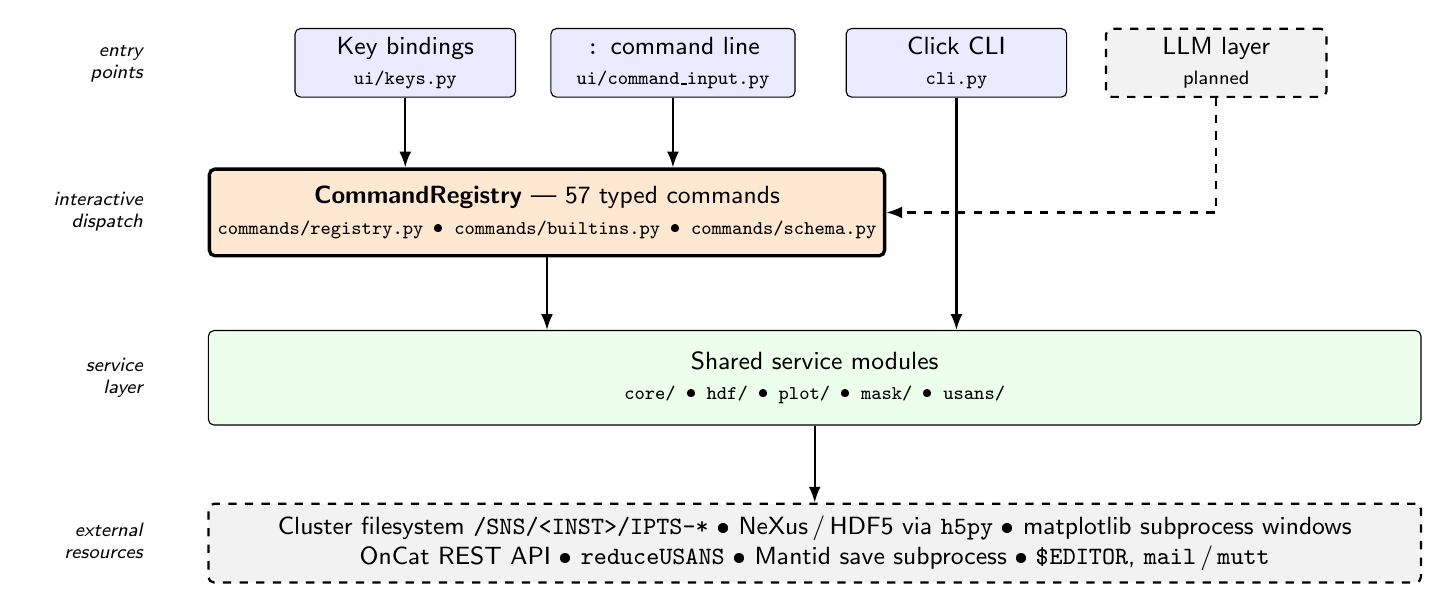
\begin{tikzpicture}[
    font=\small\sffamily,
    box/.style={draw, rounded corners=2pt, minimum height=8mm, align=center,
                inner sep=3pt},
    ui/.style={box, fill=blue!8},
    reg/.style={box, fill=orange!18, very thick},
    svc/.style={box, fill=green!8},
    ext/.style={box, fill=gray!10, dashed, thick},
    lbl/.style={font=\scriptsize\sffamily\itshape, text=black},
    flow/.style={-{Latex[length=2mm]}, thick},
    planned/.style={-{Latex[length=2mm]}, thick, dashed},
  ]

  % --- Entry points -------------------------------------------------------
  \node[ui, minimum width=28mm] (keys) at (-5.0, 5.2)
    {Key bindings\\\scriptsize\ttfamily ui/keys.py};
  \node[ui, minimum width=31mm] (cmdl) at (-1.6, 5.2)
    {\texttt{:} command line\\\scriptsize\ttfamily ui/command\_input.py};
  \node[ui, minimum width=28mm] (cli) at (2.0, 5.2)
    {Click CLI\\\scriptsize\ttfamily cli.py};
  \node[ext, minimum width=28mm] (llm) at (5.3, 5.2)
    {LLM layer\\\scriptsize planned};

  \node[lbl, anchor=east] at (-8.0, 5.2)
    {\begin{tabular}{r}entry\\points\end{tabular}};

  % --- Interactive registry ---------------------------------------------
  \node[reg, minimum width=77mm, minimum height=11mm] (registry) at (-3.2, 3.3)
    {\textbf{CommandRegistry} --- 57 typed commands\\
     \scriptsize\ttfamily commands/registry.py \textbullet\ commands/builtins.py
     \textbullet\ commands/schema.py};
  \node[lbl, anchor=east] at (-8.0, 3.3)
    {\begin{tabular}{r}interactive\\dispatch\end{tabular}};

  % --- Shared service layer ----------------------------------------------
  \node[svc, minimum width=15.4cm, minimum height=12mm] (services) at (0.2, 1.2)
    {Shared service modules\\
     \scriptsize\ttfamily core/ \textbullet\ hdf/ \textbullet\ plot/
     \textbullet\ mask/ \textbullet\ usans/};
  \node[lbl, anchor=east] at (-8.0, 1.2)
    {\begin{tabular}{r}service\\layer\end{tabular}};

  % --- External resources -------------------------------------------------
  \node[ext, minimum width=15.4cm, minimum height=10mm] (extern) at (0.2, -0.9)
    {Cluster filesystem \texttt{/SNS/<INST>/IPTS-*} \textbullet\ NeXus\,/\,HDF5
     via \texttt{h5py} \textbullet\ matplotlib subprocess windows\\
     OnCat REST API \textbullet\ \texttt{reduceUSANS} \textbullet\ Mantid save
     subprocess \textbullet\ \texttt{\$EDITOR}, \texttt{mail}\,/\,\texttt{mutt}};
  \node[lbl, anchor=east] at (-8.0, -0.9)
    {\begin{tabular}{r}external\\resources\end{tabular}};

  % --- Arrows -------------------------------------------------------------
  \draw[flow] (keys) -- (keys |- registry.north);
  \draw[flow] (cmdl) -- (cmdl |- registry.north);
  \draw[planned] (llm.south) |- (registry.east);
  \draw[flow] (registry) -- (registry |- services.north);
  \draw[flow] (cli) -- (cli |- services.north);
  \draw[flow] (services) -- (extern);

\end{tikzpicture}
}
  \longcaption{Layered architecture of sansdir.}{Key bindings and the
  interactive command line use one command registry. The \ac{cli} uses a
  separate Click path to the same service functions, and the natural-language
  layer is planned but not implemented. Reusable data operations are kept in
  service modules, while the application and interface modules coordinate the
  current session and views.}
  \label{fig:arch}
\end{figure}

The Textual application object keeps presentation and session state, including
the active pane, cursor and tags, and the modal screen stack. Interface modules
also use several lightweight helpers directly for file listings, history, and
read-only HDF views. The larger data operations are kept in reusable modules so
that they can be tested without creating a terminal application.

\subsection{THE COMMAND REGISTRY}
\label{sec:registry}

The registry is the main design decision for the interactive interface. Each
interactive action---change directory, tag, copy, plot, extract metadata, search
the catalog, create a mask---is a \texttt{Command} object. The object contains a
dotted name, a one-sentence description, a tuple of typed parameters, a handler,
optional aliases and examples, and a \texttt{danger} flag for destructive
operations. Each parameter is also a typed object. It has a name, a type from a
fixed vocabulary (\texttt{path}, \texttt{glob},
\texttt{string}, \texttt{int}, \texttt{float}, \texttt{bool}, \texttt{enum},
\texttt{files}), a description, a required flag, a default, and---for
enumerations---a list of permitted values.

Validation occurs when a command is constructed and when it is dispatched. A
parameter with an unknown type, or an enumeration without choices, raises an
error when the command is built. Therefore, a malformed command definition
fails during import instead of when a user first presses the key. During
dispatch, an unknown keyword argument or a missing required argument raises
\texttt{TypeError} before the handler runs.

Handlers can be synchronous or asynchronous. \texttt{dispatch} is asynchronous
and awaits the result when the handler is awaitable. Thus, callers use one
calling convention for both types of handlers. A synchronous convenience
wrapper is provided for call sites outside an event loop. It raises an error if
it is called from inside an event loop.

Version 0.10.2 registers 57 commands. Appendix~\ref{sec:appcommands} lists them
in full.

\subsection{DISPATCH PATHS}

Table~\ref{tab:dispatch} shows the two implemented callers of the registry and
two related interfaces. Key bindings and the interactive command line dispatch
through the registry. The \ac{cli} uses the same service modules through a
separate Click path, and the \ac{llm} layer is planned. Some interface modules
also call read-only helpers directly when they build or update a view.

\begin{table}[ht]
  \centering
  \caption{Interfaces related to the command registry}
  \label{tab:dispatch}
  \small
  \begin{tabular}{p{0.20\textwidth} p{0.72\textwidth}}
    \toprule
    Caller & Path \\
    \midrule
    Key binding &
      \texttt{ui/keys.py} maps \key{F6} to \cmd{ui.copy\_tagged}, resolves the
      active pane's selection and the inactive pane's directory into keyword
      arguments, and dispatches. \\
    Command line &
      \texttt{ui/command\_input.py} parses \texttt{cd /SNS/EQSANS} into the
      command name \cmd{nav.cd} and the argument \texttt{path}, then
      dispatches. \\
    \Ac{cli} &
      \texttt{sansdir extract -k ...} builds arguments in a separate Click
      dispatch path and calls the same extraction service used by the
      interactive dialog. \\
    \Ac{llm} layer &
      Planned, not implemented. The registry already exports a \ac{json} tool
      schema; a natural-language front end would emit command names with typed
      arguments, display them for confirmation, and dispatch. \\
    \bottomrule
  \end{tabular}
\end{table}

This design has three practical benefits. First, key bindings and the
interactive command line use the same commands, while the \ac{cli} reuses the
same underlying service functions. Second, the help overlay is generated from
registry metadata instead of being maintained by hand.
Figure~\ref{fig:help} shows this generated output. Third, the exported schema
provides a defined input for a future natural-language caller.

\begin{figure}[ht]
  \centering
  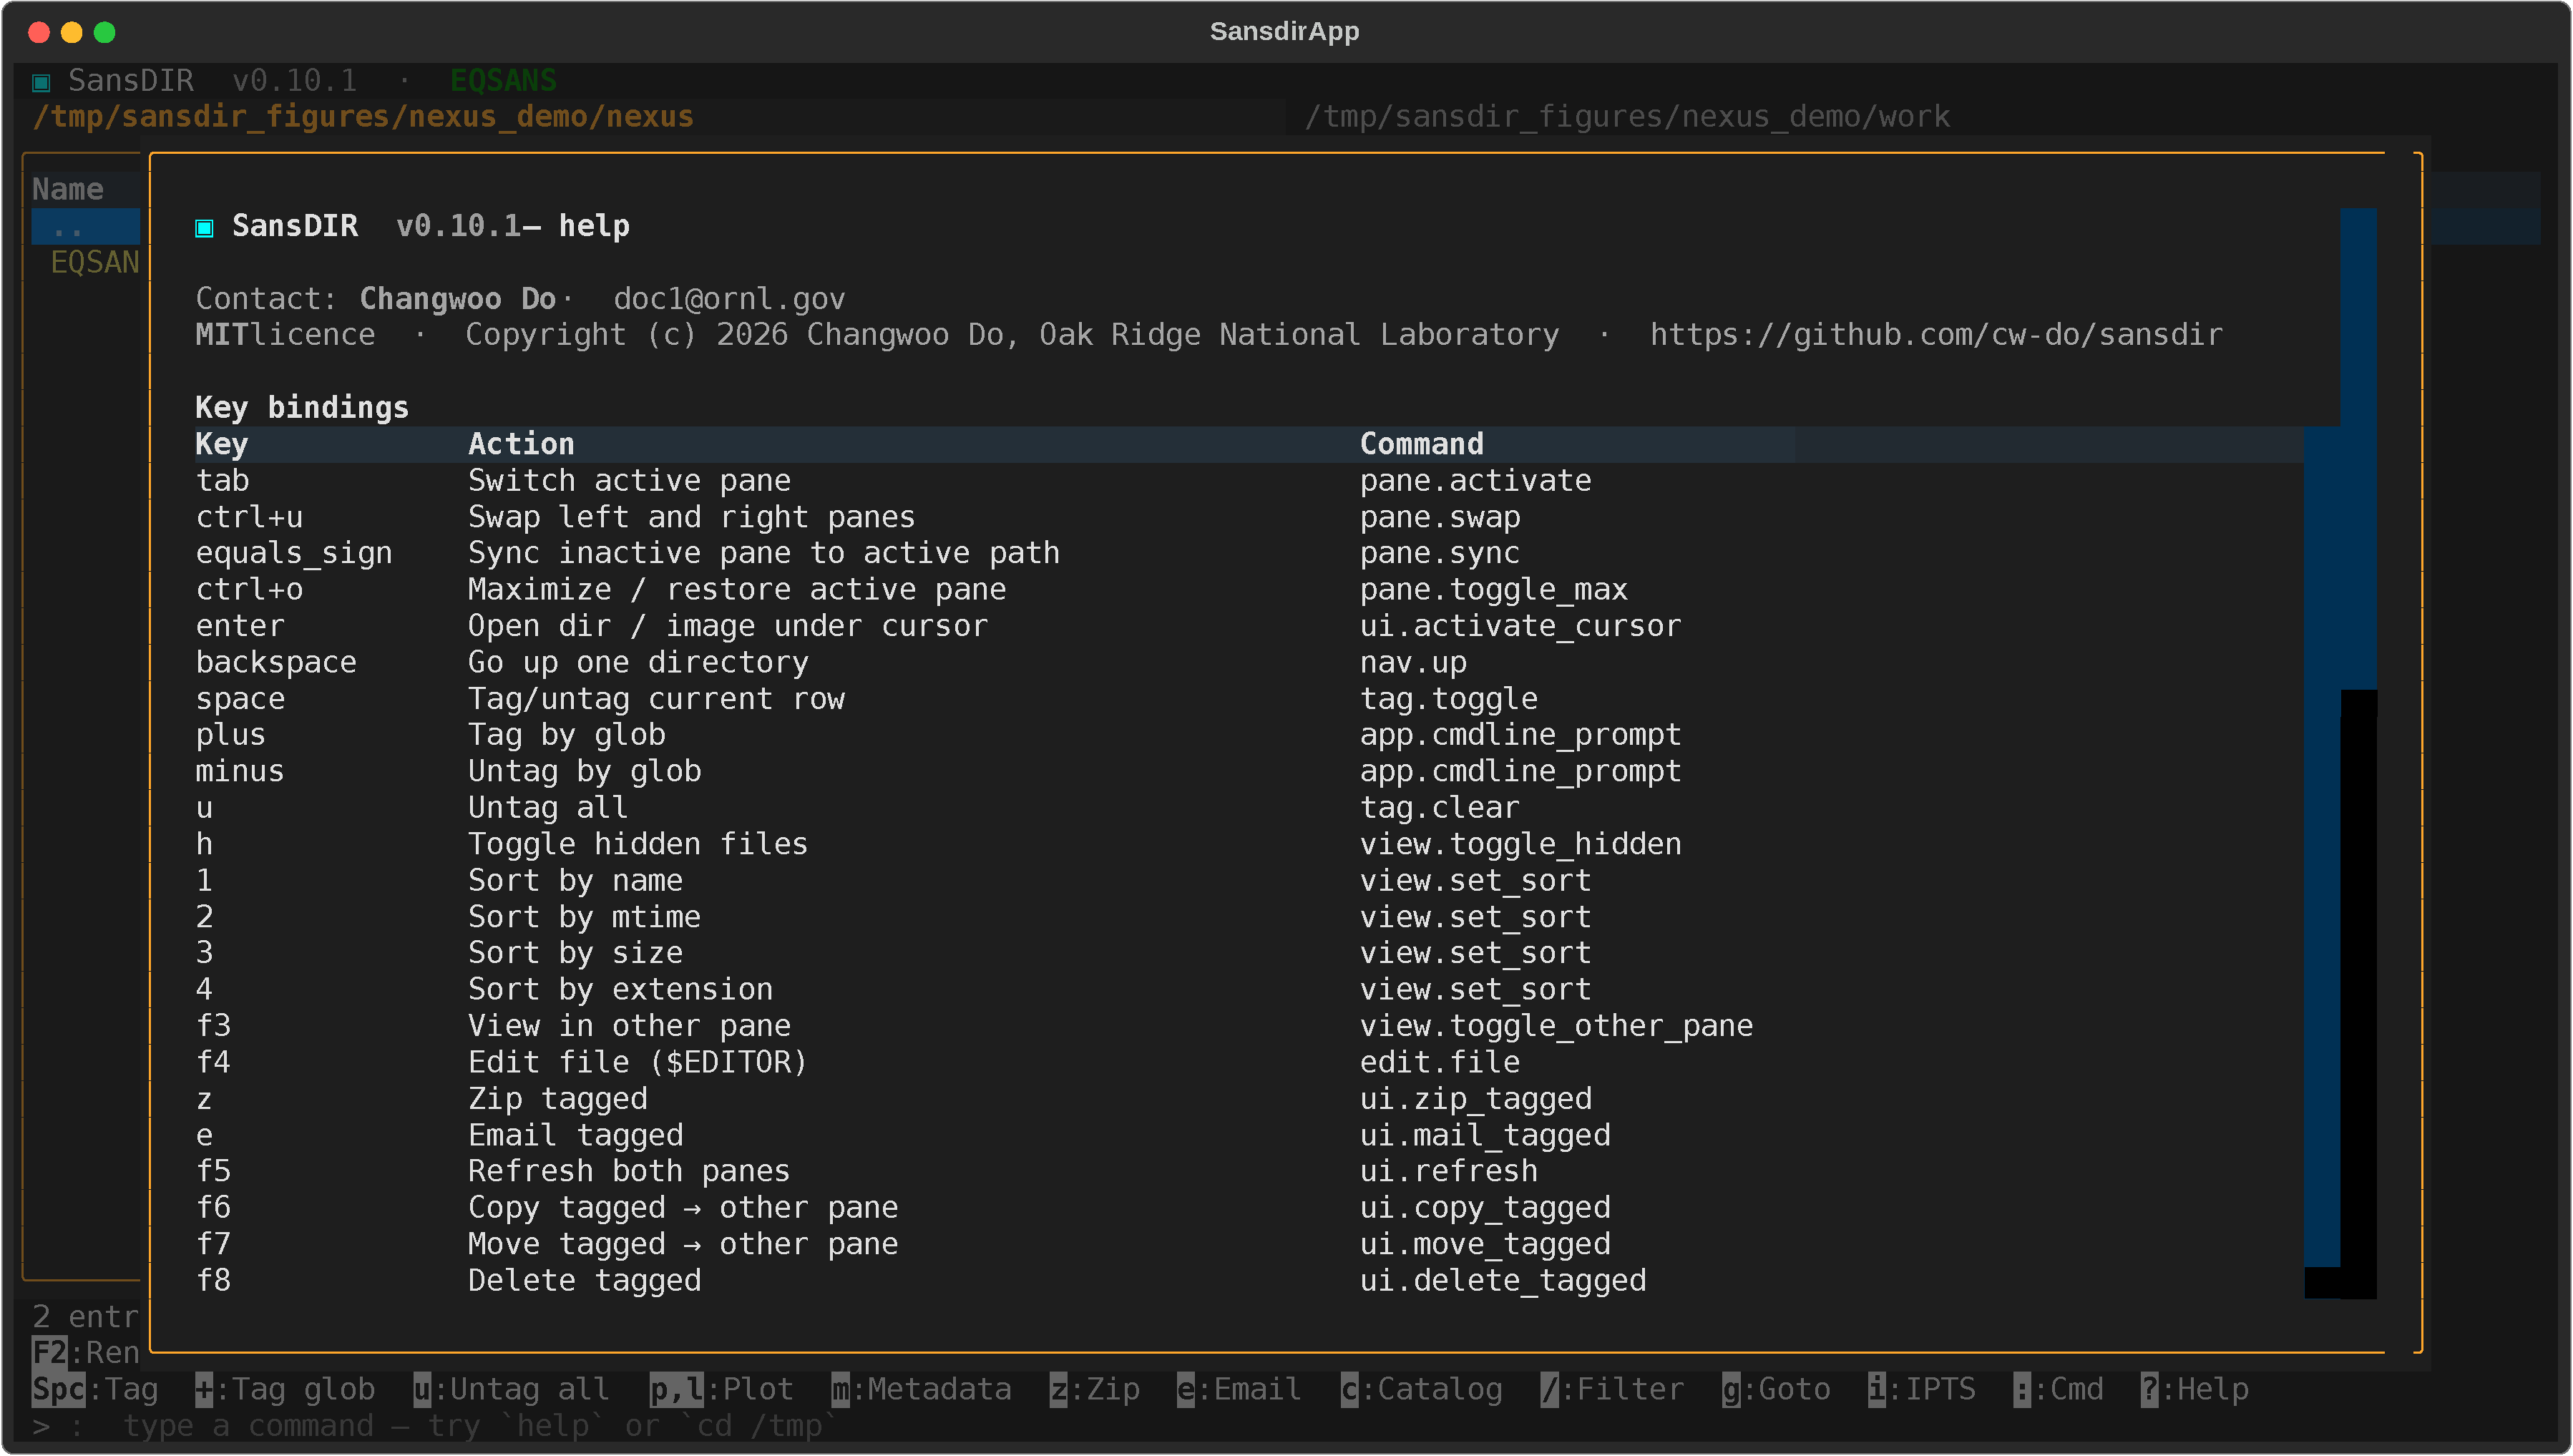
\includegraphics[width=\textwidth]{figures/help-overlay.pdf}
  \longcaption{The help overlay, generated from the registry.}{Each row shows a
  keystroke, its readable action, and the underlying command name. The third
  column shows the connection between the two interfaces. A key action can also
  be entered as a typed command. A compatible command that needs no unresolved
  arguments can be assigned to a key.}
  \label{fig:help}
\end{figure}

\subsection{KEY BINDINGS AS DATA}

The key map is a list of immutable \texttt{KeyBinding} records. Each record has
a key, a command, a description, and an optional \emph{argument resolver}. The
resolver is a small named function that converts the application state into the
keyword arguments required by the command. For example, the resolver for
\key{m} obtains the path under the cursor in the active pane and returns it as
the \texttt{path} argument for \cmd{hdf.show\_keys}.

Python can define a one-line helper function without a name (a \emph{lambda}),
but this function appears only as \texttt{<lambda>} in an error message. Each
resolver is therefore an ordinary function with a descriptive name. The error
traceback and help overlay can then identify the resolver. The default map has
48 bindings, and 38 of them are shown in the help overlay. The remaining
bindings are duplicate encodings of the same key. These duplicates are needed
because terminals report some keys differently. For example, most terminals
report the equals sign as \texttt{equals\_sign}, while others report
\texttt{=}. Both forms are registered, but the duplicate entry is hidden from
help.

A test checks that every binding names a command in the fully bound registry.
Therefore, a typo in the key map fails in \ac{ci} instead of at runtime.

Users can replace or add bindings through the \texttt{[keys]} section of the
configuration file. An entry with an unknown command is removed at startup with
a notification, instead of stopping the launch.

\subsection{THE COMMAND LINE PARSER}

The \key{:} line accepts registered command names and aliases with positional
and keyword arguments. It does not interpret natural language and does not use
\texttt{eval} or \texttt{exec}. This is a safety boundary. Natural-language
input is reserved for the future \ac{llm} layer, which can produce only
registry-defined commands with typed arguments.

Aliases keep the typed interface short. \cmd{nav.cd} is available as
\texttt{cd}, \cmd{hdf.batch\_extract} as \texttt{extract},
\cmd{oncat.search} as \texttt{ipts}, and \cmd{shell.run} as \texttt{!}.
Command history persists across sessions.

\subsection{STARTUP BUDGET AND LAZY IMPORTS}
\label{sec:startup}

The startup budget is 300~ms. The measured value in this report is for
\texttt{sansdir --help}, not for the first paint of the \ac{tui}. This path was
measured again after \ac{usans} reduction and desmearing were added. Its median
end-to-end wall-clock time on an analysis node is about 120~ms. About 40~ms is
used to start the Python interpreter, and about 40~ms is used to import the
command module. The best case is near 60~ms. The new features did not increase
this value because the help path does not import them. A check confirms that
\texttt{numpy}, \texttt{h5py}, \texttt{matplotlib}, Textual, and \texttt{httpx}
are absent from \texttt{sys.modules} after \texttt{import sansdir.cli}. The
\ac{tui} first-paint time has not been measured for this report.

The \ac{cli} imports only \texttt{click} and the version constant at module
scope. Textual, matplotlib, \texttt{h5py}, \texttt{httpx}, and the registry are
imported inside the subcommands that need them. Therefore, the commands
\texttt{sansdir version} and \texttt{sansdir --help} do not load the scientific
stack. The \ac{tui} loads Textual at startup but delays matplotlib and
\texttt{h5py} until the first plot or metadata operation.

The \texttt{--help} startup time is checked after a change to the import graph.

\subsection{CONCURRENCY MODEL}

Three mechanisms keep the interface responsive:

\begin{itemize}
  \item \textbf{Thread offload.} Blocking library calls, mainly \texttt{h5py}
    reads, run through \texttt{asyncio.to\_thread}. The \ac{hdf} key search in
    Section~\ref{sec:hdfsearch} is an example. Walking through a large raw NeXus
    file takes seconds, so the walk runs on a thread. The result is stored in the
    screen object for later queries.
  \item \textbf{Textual workers.} Longer interactive operations run as
    background workers, while the event loop continues to process keystrokes.
    For example, the mask editor launcher waits for the editor subprocess in a
    worker and refreshes both panes when the editor saves and exits.
  \item \textbf{Subprocesses.} Plot windows run in a separate process. This is
    the only reliable way to give matplotlib its own \ac{gui} event loop without
    competing with the Textual event loop.
\end{itemize}

\subsection{REPOSITORY LAYOUT}

Table~\ref{tab:layout} lists the package structure. The implementation contains
approximately 18,500 lines in 66 Python modules.

\begin{table}[ht]
  \centering
  \caption{Package structure}
  \label{tab:layout}
  \small
  \begin{tabular}{l p{0.68\textwidth}}
    \toprule
    Path & Contents \\
    \midrule
    \texttt{cli.py} & Click entry point; \texttt{tui}, \texttt{extract},
      \texttt{mask}, \texttt{usans}, and \texttt{version} subcommands. \\
    \texttt{app.py} & The Textual application shell. \\
    \texttt{config.py} & Configuration loader for \ac{toml}
      \autocite{toml} (``Tom's Obvious Minimal Language,'' the format's real
      name), read with the standard-library \texttt{tomllib}. \\
    \texttt{commands/} & \texttt{registry.py} (the \texttt{Command} model and
      dispatch), \texttt{builtins.py} (56 app-bound registrations plus
      \texttt{app.quit}, 57 total),
      \texttt{parser.py} (the \key{:} line), \texttt{schema.py} (\ac{json} tool
      schema export). \\
    \texttt{core/} & \texttt{filesystem.py} (listing and sorting),
      \texttt{fileops.py} (copy, move, delete), \texttt{archive.py},
      \texttt{mailer.py}, \texttt{oncat.py}, \texttt{history.py},
      \texttt{instrument.py} (\ac{sans}/\ac{usans} mode resolution). \\
    \texttt{hdf/} & \texttt{reader.py} (safe open, tree walk, value previews),
      \texttt{metadata.py}, \texttt{batch.py} (parallel extraction). \\
    \texttt{plot/} & \texttt{detect.py} (file-kind classification),
      \texttt{ascii1d.py}, \texttt{ascii2d.py}, \texttt{tile.py},
      \texttt{generic.py}, \texttt{image.py}, \texttt{hdf5\_detector.py},
      \texttt{backend.py}, \texttt{window.py} (the plot subprocess). \\
    \texttt{usans/} & \texttt{grouping.py} (title blocks), \texttt{reconcile.py}
      (scan counts derived from disk), \texttt{table.py} (the setup \ac{csv}),
      \texttt{catalog.py} (table and notes), \texttt{runner.py} (invoking the
      external engine), \texttt{desmear.py} (truncated Abel inversion) and
      \texttt{desmear\_io.py} (reading and writing curves). Pure; imports no
      interface or network module. \\
    \texttt{mask/} & \texttt{core.py} (shapes and the mask builder),
      \texttt{detector.py}, \texttt{banktube.py}, \texttt{writers.py},
      \texttt{mantid\_writer.py}, \texttt{gui.py}, \texttt{api.py}. \\
    \texttt{ui/} & \texttt{panel.py}, \texttt{pane\_slot.py},
      \texttt{keys.py}, \texttt{command\_input.py}, \texttt{dialogs.py},
      \texttt{hdf\_tree.py}, \texttt{run\_catalog.py},
      \texttt{oncat\_browser.py}, \texttt{help.py}, \texttt{statusbar.py},
      \texttt{titlebar.py}, \texttt{pathbar.py}, \texttt{key\_hint\_bar.py},
      \texttt{inline\_viewer.py}, \texttt{prompt\_panel.py}. \\
    \bottomrule
  \end{tabular}
\end{table}

%%%%%%%%%%%%%%%%%%%%%%%%%%%%%%%%%%%%%%%%%%%%%%%%%%%%%%%%%%%%%%%%%%%%%%%%%%%%%%%
% 4. USER INTERFACE
%%%%%%%%%%%%%%%%%%%%%%%%%%%%%%%%%%%%%%%%%%%%%%%%%%%%%%%%%%%%%%%%%%%%%%%%%%%%%%%
\section{THE USER INTERFACE}
\label{sec:ui}

\subsection{SCREEN ANATOMY}

Figure~\ref{fig:panes} shows a running session. From top to bottom, the screen
contains a title bar with the program name and version; a two-part path bar that
shows the working directory of each pane and highlights the active path; the two
file panes; a status line with the entry count and number of tagged files; a
two-row key hint bar in the Norton Commander style; and the command line.

\begin{figure}[ht]
  \centering
  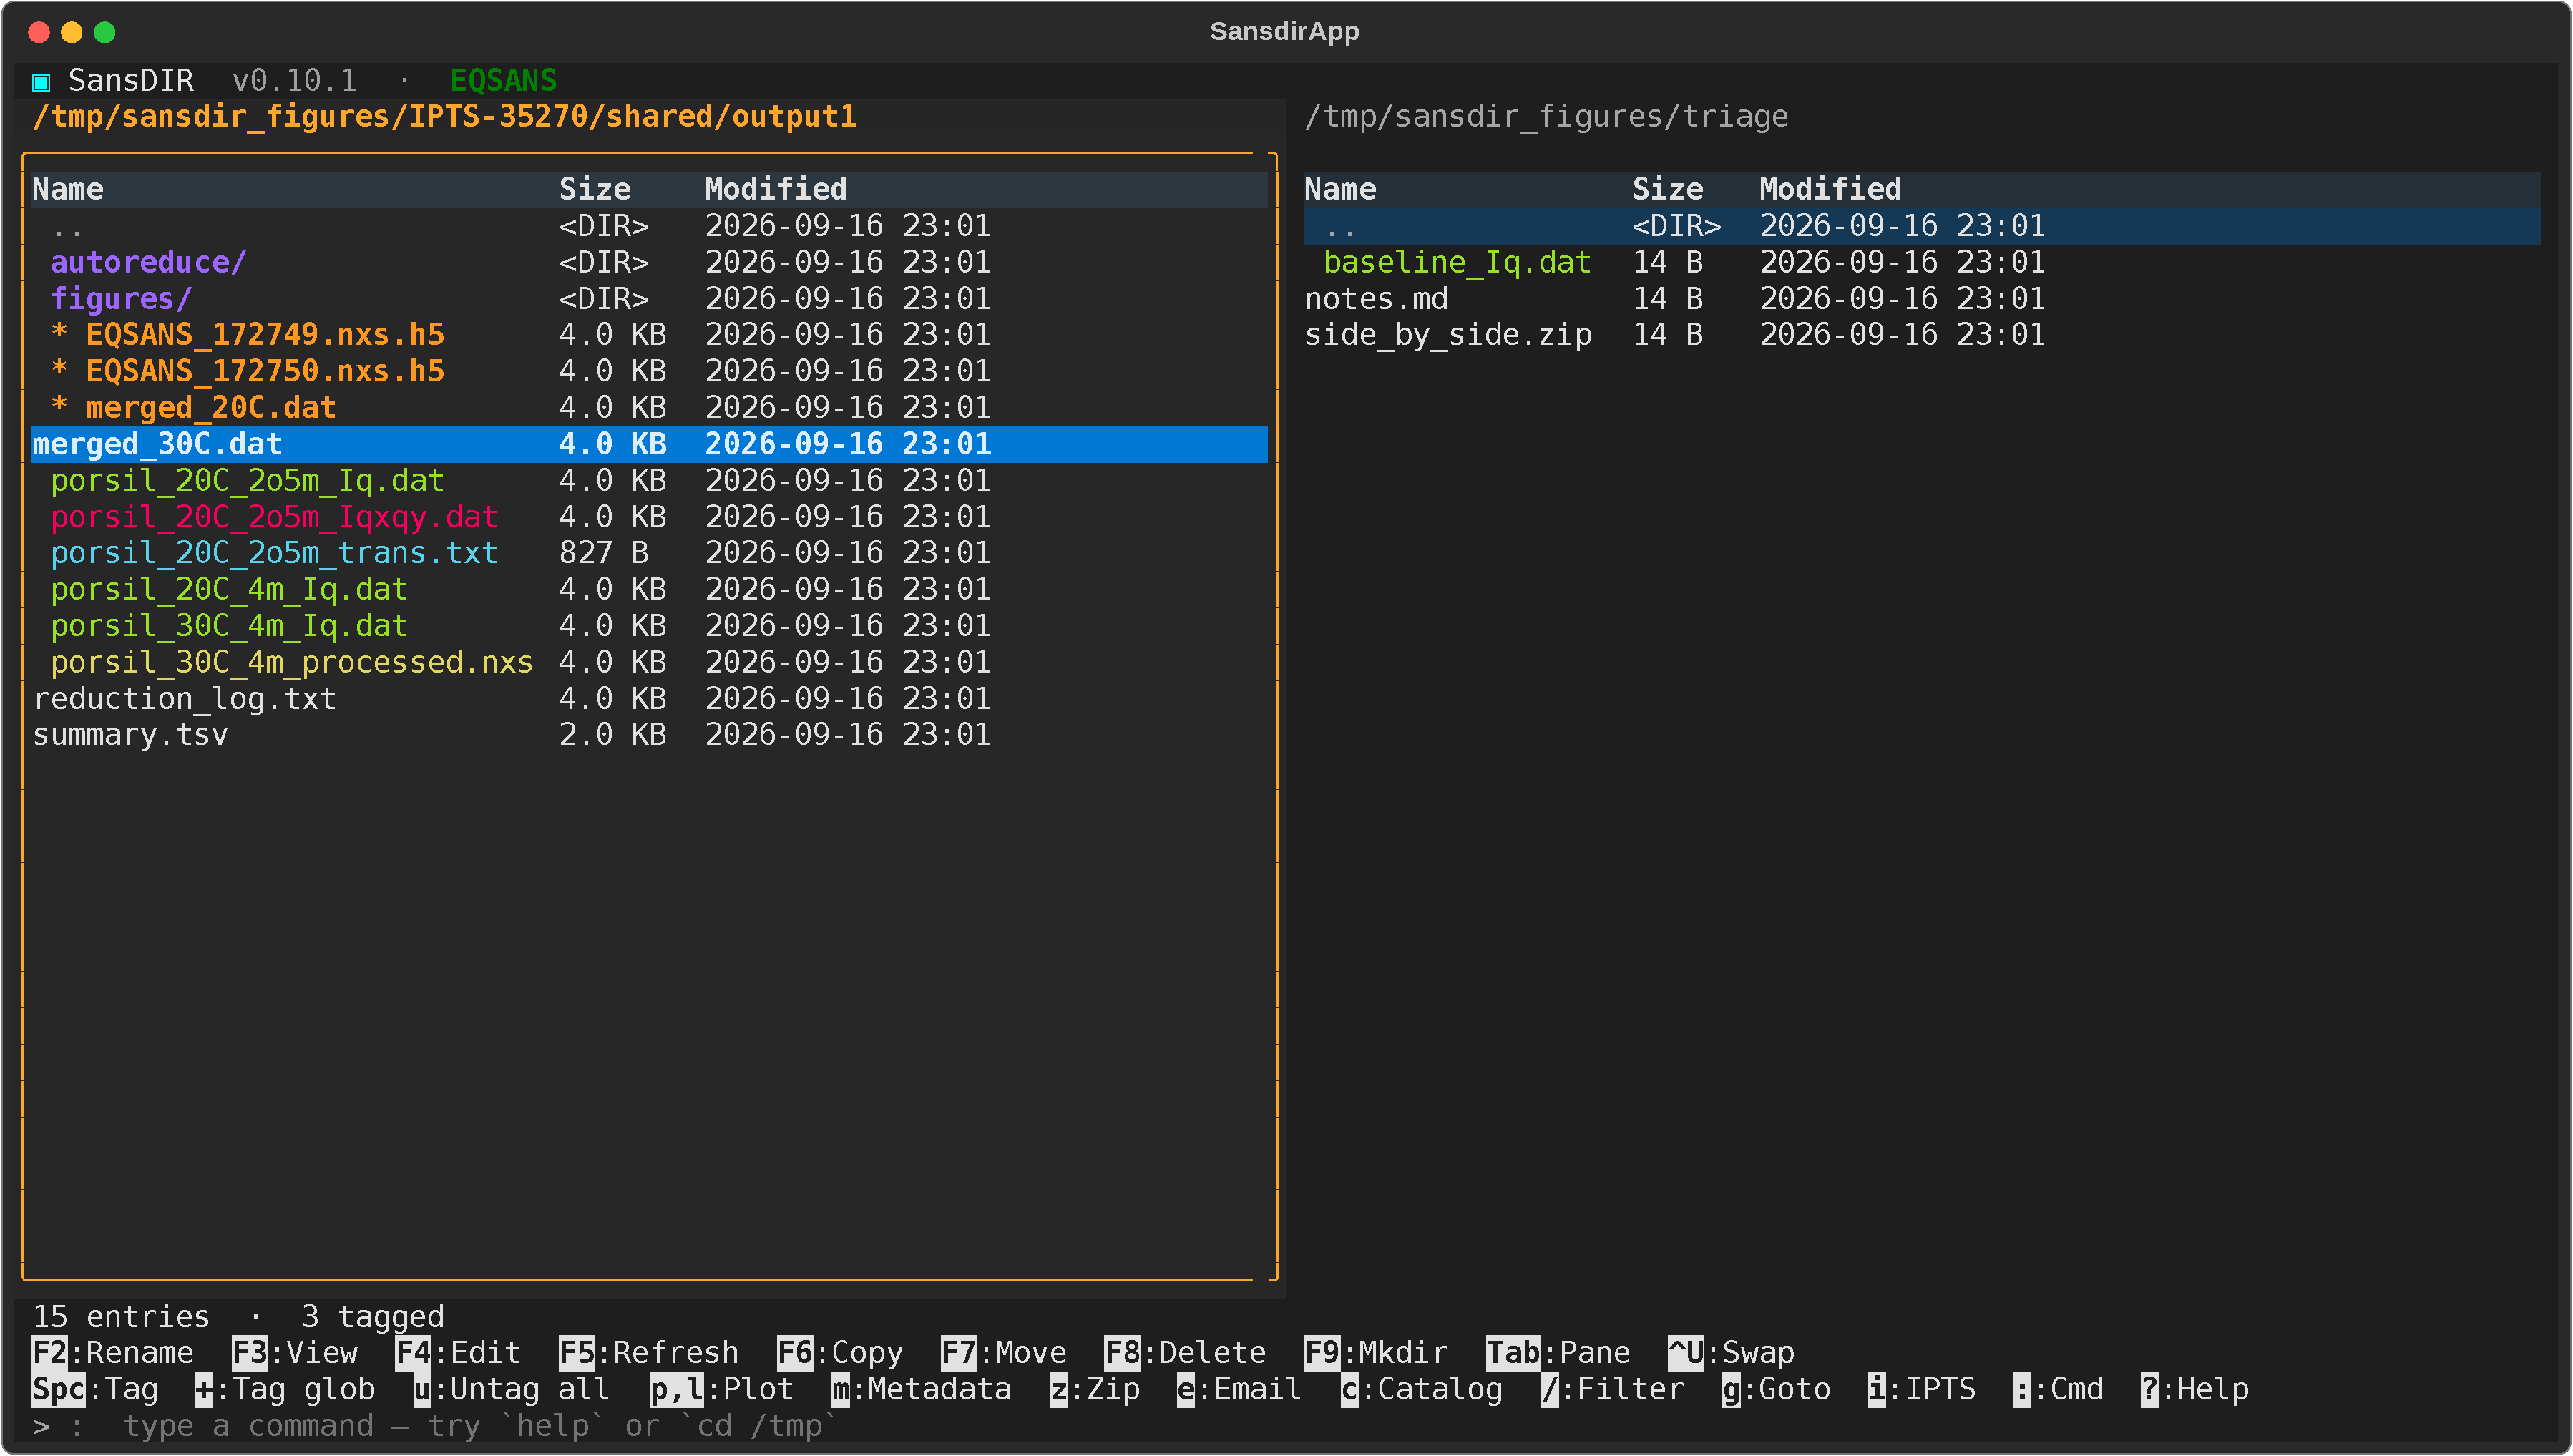
\includegraphics[width=\textwidth]{figures/tui-panes.pdf}
  \longcaption{The dual-pane interface.}{The highlighted border and path show
  that the left pane is active. Three files are tagged. They have a leading
  asterisk and bold text, and the status line gives the count. Color identifies
  the file kind. Directories, one-dimensional reduced data, two-dimensional
  reduced data, transmission files, and NeXus files each have a different
  color.}
  \label{fig:panes}
\end{figure}

The path bar displays the \texttt{/gpfs/neutronsfs/instruments} prefix as
\texttt{/SNS}. Users normally write and recognize the location in this form.
The two paths refer to the same mount, so this display does not change the
location.

\subsection{PANES AND ACTIVATION}

The two panes are instances of the same widget class, but they have independent
states: working directory, cursor position, tag set, sort key, and filter. One
pane is active at a time and is identified by its border color. \key{Tab}
changes the active pane.

Several commands act on both panes. \key{Ctrl+U} swaps their contents and quickly
reverses the direction of a copy. \key{=} changes the inactive pane to the
directory of the active pane. This is the usual preparation for an operation in
the same directory. \key{Ctrl+O} expands the active pane to full width, and a
second press restores both panes. Full width is a toggle and not the default
because the program is designed around two panes.

The run catalog described in Section~\ref{sec:oncat} always appears in the right
pane, independent of which pane was active when it was requested. This keeps the
layout consistent. The catalog remains on the right, and \key{Ctrl+U} swaps file
panes without changing it.

\subsection{FILE LISTING AND COLOR CODING}

Each pane lists name, size, and modification time. Directories sort first.
Sorting is by name, modification time, size, or extension, selected with the
number keys \key{1} through \key{4}. Hidden files are suppressed by default and
toggled with \key{h}. Symbolic links are followed but flagged.

Color identifies the file kind and helps the user scan a directory quickly
(Table~\ref{tab:colors}).

\begin{table}[ht]
  \centering
  \caption{File-kind color coding in the panes}
  \label{tab:colors}
  \small
  \begin{tabular}{l l}
    \toprule
    Kind & Rendering \\
    \midrule
    Directory & Bold blue \\
    Symbolic link & Cyan \\
    \texttt{*Iq*.dat}, one-dimensional reduced & Green \\
    \texttt{*Iqxqy*.dat}, two-dimensional reduced & Magenta \\
    \texttt{*trans*.txt}, transmission & Cyan \\
    \texttt{*.nxs.h5} and \texttt{*.nxs}, NeXus & Bright yellow \\
    Executable & Bold red \\
    Tagged row & Bold yellow with a leading asterisk \\
    \bottomrule
  \end{tabular}
\end{table}

\subsection{TAGGING}

Tags select files for every multi-file operation. \key{Space} changes the tag
on the row under the cursor. \key{+} asks for a glob and tags each visible entry
that matches it. \key{-} removes tags by glob, and \key{u} removes all tags in
the active pane. Each pane has its own tags, which are cleared when the pane
changes directory.

All operations follow the same rule. If the active pane has tagged files, the
operation acts on them. Otherwise, it acts on the file under the cursor. Thus, a
single-file operation does not require a tag, and a multi-file operation does
not require a separate ``select mode.''

\key{/} filters the active pane by substring. It can be used with glob tagging:
filter to a subset, tag all visible files, and then perform the operation.

\subsection{COMMAND LINE AND HISTORY}

The command line is always visible at the bottom of the screen. \key{:} moves
the focus to it. It accepts any registered command name or alias. Some shortcut
keys fill the command line instead of immediately performing an action.
\key{+} opens it with \texttt{tag.glob}, \key{g} with \texttt{cd}, and \key{F9}
with \texttt{mkdir}. Therefore, the connection between a key and its command is
visible during use and not only in the help overlay.

History persists across sessions in the cache directory.

\subsection{HELP OVERLAY}

\key{?} opens the help overlay in Figure~\ref{fig:help}. The program generates
it from the registry and key map at runtime. Therefore, the overlay includes
user key rebindings and remains consistent with the code.

%%%%%%%%%%%%%%%%%%%%%%%%%%%%%%%%%%%%%%%%%%%%%%%%%%%%%%%%%%%%%%%%%%%%%%%%%%%%%%%
% 5. NAVIGATION AND FILE OPERATIONS
%%%%%%%%%%%%%%%%%%%%%%%%%%%%%%%%%%%%%%%%%%%%%%%%%%%%%%%%%%%%%%%%%%%%%%%%%%%%%%%
\section{NAVIGATION AND FILE OPERATIONS}
\label{sec:fileops}

\subsection{NAVIGATION}

Table~\ref{tab:nav} lists the navigation keys. The action of \key{Enter} depends
on the selected item. It opens a directory, opens an image viewer, previews a
text file in the other pane, or plots the run under the cursor in the run
catalog.

\begin{table}[ht]
  \centering
  \caption{Navigation keys}
  \label{tab:nav}
  \small
  \begin{tabular}{l l}
    \toprule
    Key & Action \\
    \midrule
    \key{Tab} & Switch the active pane \\
    Arrow keys, \key{j} \key{k} & Move the cursor \\
    \key{Enter} & Descend into a directory, open an image, preview text, or plot
      a catalog row \\
    \key{Backspace} & Ascend one directory \\
    \key{g} & Prompt for a path \\
    \key{G} & Full-screen directory-tree browser \\
    \key{/} & Filter the active pane by substring \\
    \key{=} & Synchronize the inactive pane to the active pane's directory \\
    \key{Ctrl+U} & Swap the two panes \\
    \key{Ctrl+O} & Maximize or restore the active pane \\
    \bottomrule
  \end{tabular}
\end{table}

\subsection{FILE OPERATION SEMANTICS}

File operations follow the Norton Commander convention. They use the selection
in the active pane, and the working directory of the \emph{inactive} pane is the
default destination. Table~\ref{tab:fkeys} lists the function-key assignments.

\begin{table}[ht]
  \centering
  \begin{threeparttable}
  \caption{Function-key file operations}
  \label{tab:fkeys}
  \small
  \begin{tabular}{l l p{0.52\textwidth}}
    \toprule
    Key & Operation & Behavior \\
    \midrule
    \key{F2} & Rename & In-place rename of the file under the cursor. \\
    \key{F3} & View & Read-only view in the opposite pane; \key{Esc} or a
      second \key{F3} closes it. \\
    \key{F4} & Edit & Opens \texttt{\$EDITOR}. \\
    \key{F5} & Refresh & Re-reads both directory listings. \\
    \key{F6} & Copy & Selection into the inactive pane, after confirmation. \\
    \key{F7} & Move & As copy, then removes the source. \\
    \key{F8} & Delete & Always confirms; uses \texttt{send2trash} where
      available. \\
    \key{F9} & Make directory & Prompts in the active pane. \\
    \key{c} & Catalog toggle & Flips the inactive pane between file list and run
      catalog.\tnote{a} \\
    \bottomrule
  \end{tabular}
  \begin{tablenotes}
    \item[a] The catalog toggle is bound to \key{c} rather than \key{F10}
    because most terminal emulators intercept \key{F10} for their own menu bar.
    The classic copy, move, and delete bindings are correspondingly shifted from
    \key{F5}--\key{F7} to \key{F6}--\key{F8} to make room for refresh.
  \end{tablenotes}
  \end{threeparttable}
\end{table}

Two behaviors were added after user feedback. After a file is deleted, the
cursor remains near its previous position. It stays on the replacement row, or
on the new last row if the deleted file was last. This makes it easier to remove
several files individually. Also, every destructive operation requires
confirmation and is logged.

\subsection{REFRESH BEHAVIOR}

Operations performed in the application, including copy, move, rename, directory
creation, batch extraction, and archive creation, refresh the affected panes
automatically. \key{F5} provides a manual refresh for external changes. These
can come from another shell session, an autoreduction job writing new output, or
delayed \ac{nfs} attribute updates.

The mask editor runs as a separate subprocess so that the interface remains
responsive. A worker waits for its exit code. If the editor reports that a file
was saved, both panes are refreshed and the new mask file appears.

\subsection{ARCHIVING AND EMAIL}

\key{z} creates a zip archive from the selection. It asks for the archive name
and uses the inactive pane's directory by default. The command line also provides
\cmd{archive.tar\_gz} for a gzip-compressed tar archive. \key{e} opens a dialog
and sends the selection as attachments through the configured \texttt{mail} or
\texttt{mutt} program.

\subsection{SHELL ESCAPE}

\cmd{shell.run}, with the alias \texttt{!}, suspends the interface and runs a
shell command. The interface returns when the command finishes. This provides
access to operations that are not implemented in the program.

%%%%%%%%%%%%%%%%%%%%%%%%%%%%%%%%%%%%%%%%%%%%%%%%%%%%%%%%%%%%%%%%%%%%%%%%%%%%%%%
% 6. PLOTTING
%%%%%%%%%%%%%%%%%%%%%%%%%%%%%%%%%%%%%%%%%%%%%%%%%%%%%%%%%%%%%%%%%%%%%%%%%%%%%%%
\section{PLOTTING}
\label{sec:plot}

\subsection{PLOTTING THE SELECTION}

\key{p} plots the active selection. It uses the tagged files when tags are
present and otherwise uses the file under the cursor. The program determines the
plot from the file, so the same key works for each supported type of \ac{sans}
data. Table~\ref{tab:plotrouting} lists the resulting plots.

\begin{table}[ht]
  \centering
  \caption{What \key{p} draws for each kind of file}
  \label{tab:plotrouting}
  \small
  \begin{tabular}{p{0.30\textwidth} p{0.60\textwidth}}
    \toprule
    Selection & Result \\
    \midrule
    \texttt{*Iq*.dat}, 2--4 columns & Logarithmic $I(q)$ plot, with error bars
      when a $\sigma_I$ column is present. Several files overlay on shared
      axes. \\
    \texttt{*trans*.txt} & Transmission $T(\lambda)$ on linear axes,
      $\lambda$ in \AA. \\
    \texttt{*Iqxqy*.dat}, 4 or 6 columns & Two-dimensional heat map; several
      files tile into one window. \\
    \texttt{*.nxs.h5} raw event file & Detector heat map of summed counts. \\
    \texttt{*.nxs} processed Mantid file & Detector heat map through the same
      view. \\
    Any other tabular file (\key{l}) & Linear plot using the header row as axis
      labels. \\
    \bottomrule
  \end{tabular}
\end{table}

Plots open in separate windows, and the terminal remains available while the
figures are open. Several figures can be shown at the same time. On a host
without a display, the figure is written as a \ac{png} under
\texttt{\hme/.cache/sansdir/plots/}, and the status bar reports its path. Thus,
the same key also works in a plain \ac{ssh} session without forwarding.

Classification does not use only the file extension. Mantid writes processed
output as \texttt{.nxs} without the \texttt{.h5} suffix, and reduced files do not
always have predictable names. A file containing \ac{hdf} data is treated as a
NeXus file regardless of its name. Column counts and header keywords distinguish
the ASCII formats.

\subsection{ONE-DIMENSIONAL PLOTS}

Reduced $I(q)$ files use logarithmic axes by default and include error bars when
a third column is present. Several tagged files are overlaid on shared axes with
a filename legend. This supports common comparisons such as one sample at two
temperatures or one measurement at two detector distances.
Figure~\ref{fig:iq} shows an example with one curve.

\begin{figure}[ht]
  \centering
  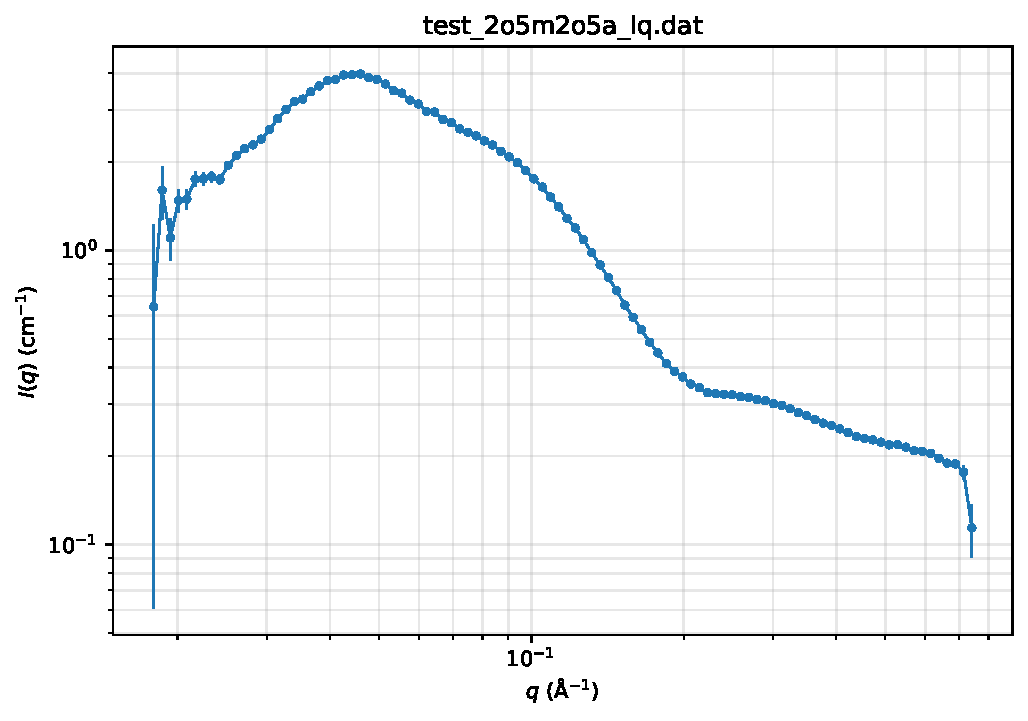
\includegraphics[width=0.78\textwidth]{figures/plot-iq.pdf}
  \longcaption{One-dimensional reduced data.}{A three-column $I(q)$ file plotted
  on logarithmic axes with error bars. Axis labels and units are applied
  automatically. This figure was produced by the same code path the \key{p} key
  invokes.}
  \label{fig:iq}
\end{figure}

Transmission files use linear axes, with wavelength in \AA{} on the abscissa and
transmission on the ordinate. The labels and title are set accordingly.

\subsection{TWO-DIMENSIONAL PLOTS}

Four- and six-column $I(q_x,q_y)$ files are drawn as heat maps on $q_x$ and
$q_y$ axes. A logarithmic color scale is used by default.

When several two-dimensional files are tagged, they are tiled in one window and
each subplot uses its filename as the title. Two color-bar modes are available.
In \emph{shared} mode, one scale is used for all panels and their intensities can
be compared directly. In \emph{independent} mode, each panel has its own scale,
which can make weak patterns more visible. Shared mode is the default because
the panels are normally being compared. The standing preference is set with
\texttt{[ui].colorbar\_mode}. One plot can override it with
\texttt{:plot.iqxqy colorbar\_mode=independent}.

Figure~\ref{fig:iqxqy-tile} shows a real temperature series in the tiled view.
It contains eight reduced $I(q_x,q_y)$ files from one sample measured from 20 to
55\,$^{\circ}$C. The whole series is selected in the file pane with one glob:
\key{+}, followed by \texttt{*C\_conf1\_Iqxqy.dat}. After \key{p} is pressed,
the files are placed in natural order, four panels per row, with one logarithmic
color scale. The temperature-dependent change in the scattering ring can then
be compared across the panels.

\begin{figure}[ht]
  \centering
  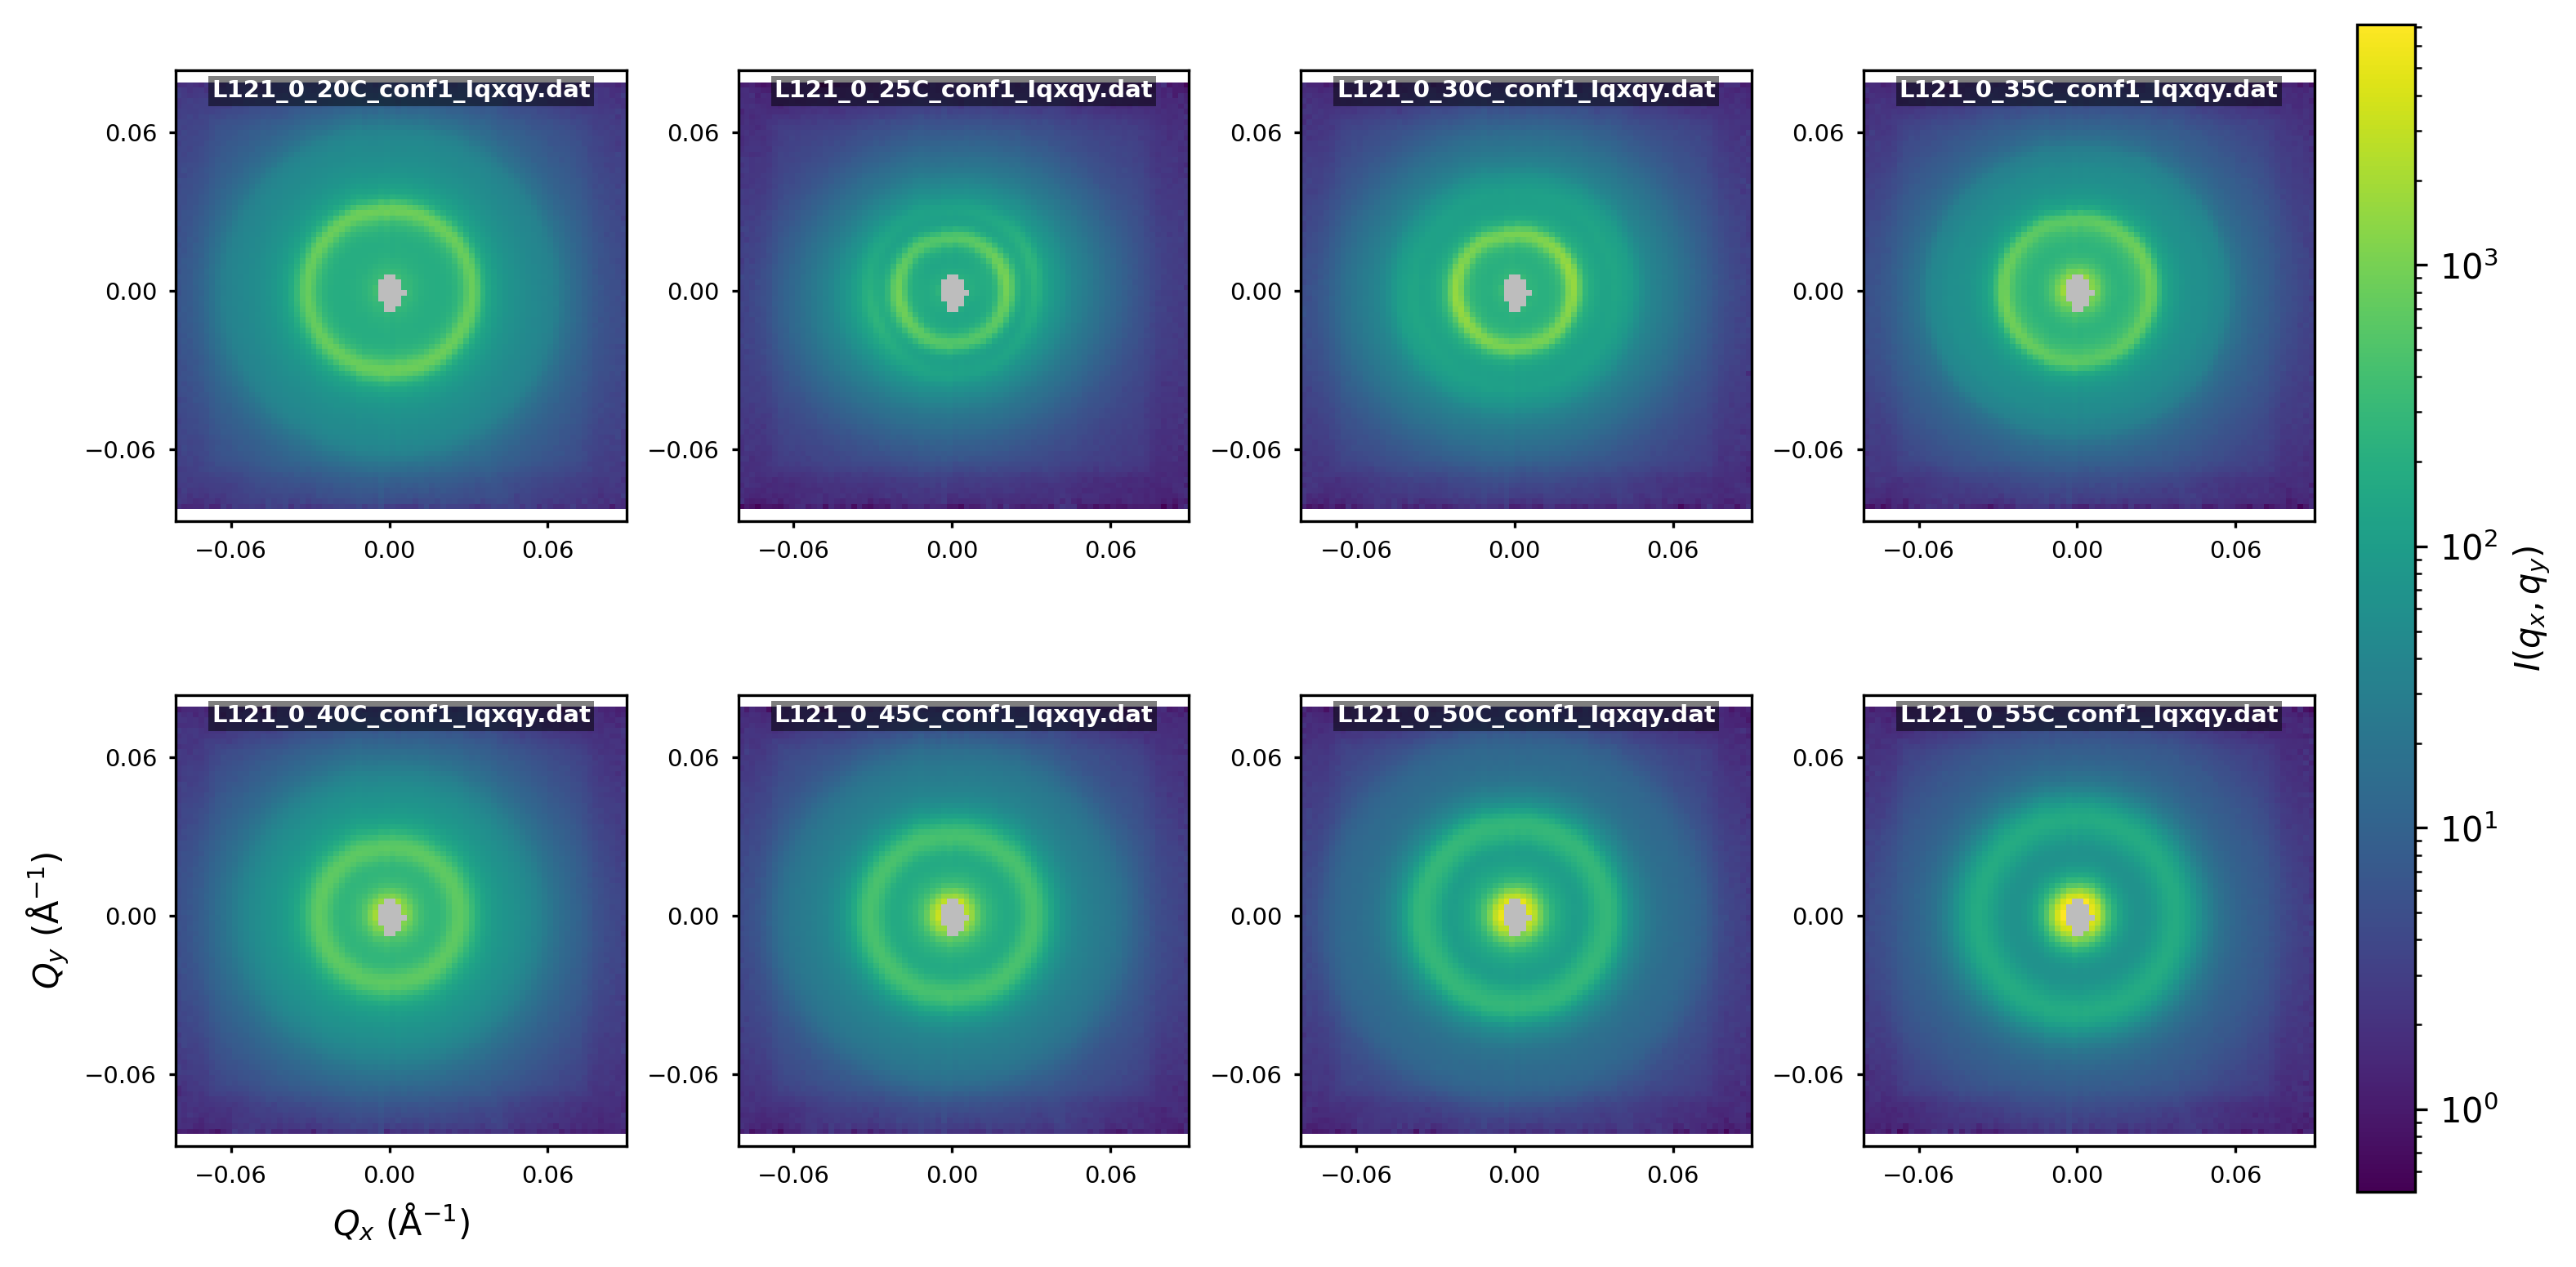
\includegraphics[width=\textwidth]{figures/plot-iqxqy-tile.png}
  \longcaption{Tiled two-dimensional plot of a temperature series.}{Eight
  reduced $I(q_x,q_y)$ files (IPTS-36552, 20--55\,$^{\circ}$C) tagged with
  one glob and plotted with \key{p}. The shared logarithmic color bar makes
  the panels directly comparable; the isotropic scattering ring contracts
  and the low-$q$ intensity grows as the sample is heated.}
  \label{fig:iqxqy-tile}
\end{figure}

\subsection{DETECTOR HEAT MAPS FROM NEXUS}

Raw EQ-SANS \autocite{eqsans} event files are rendered as a
$256\times192$ detector image, as shown in Figure~\ref{fig:detector}. Processed
Mantid files---including wavelength-banded \texttt{drtsans} output and
event-workspace masks---render through the same view.

\begin{figure}[ht]
  \centering
  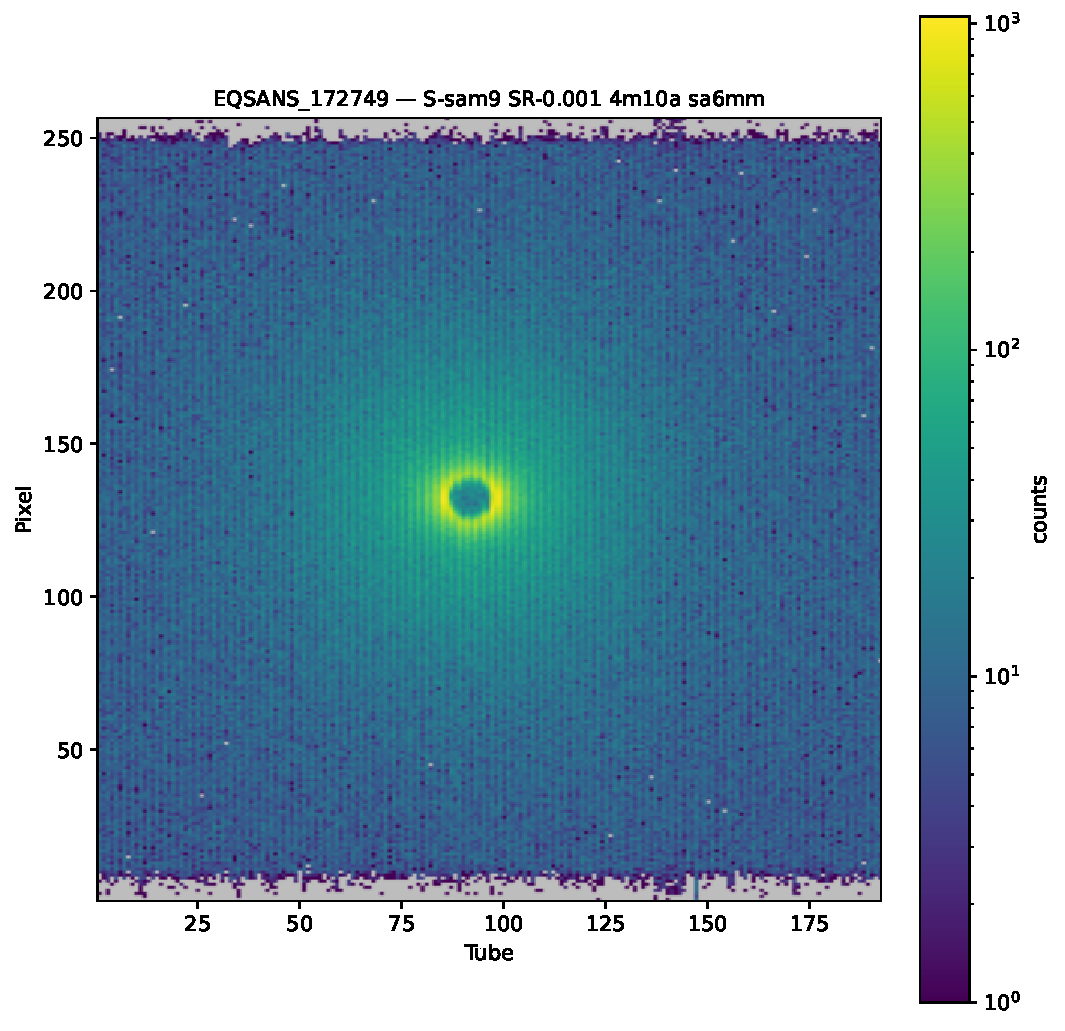
\includegraphics[width=0.72\textwidth]{figures/plot-detector.pdf}
  \longcaption{Detector heat map from a raw NeXus event file.}{Counts summed over
  all events and reordered into the physical tube-and-pixel layout, on a
  logarithmic color scale. The beam stop is visible at the center of the direct
  beam. The reconstruction is performed entirely in \texttt{numpy}; no Mantid
  runtime is involved.}
  \label{fig:detector}
\end{figure}

The image is reconstructed from the event arrays without starting Mantid.
Therefore, the detector view is available on hosts without a Mantid environment
and while a Mantid installation is being upgraded.

\subsection{GENERIC TABULAR PLOTS}

\key{l} plots whitespace-, comma-, or tab-delimited tables on linear axes and
uses the header row for axis labels. This operation can be used with the batch
metadata extractor in Section~\ref{sec:meta}. For example, the user can extract
temperature against time across a run series and plot the resulting table in the
same program.

\key{Enter} opens static images, including \ac{png}, JPEG, and TIFF files, in a
matplotlib window. This can be used for figures written by autoreduction.

%%%%%%%%%%%%%%%%%%%%%%%%%%%%%%%%%%%%%%%%%%%%%%%%%%%%%%%%%%%%%%%%%%%%%%%%%%%%%%%
% 7. METADATA
%%%%%%%%%%%%%%%%%%%%%%%%%%%%%%%%%%%%%%%%%%%%%%%%%%%%%%%%%%%%%%%%%%%%%%%%%%%%%%%
\section{METADATA INSPECTION AND EXTRACTION}
\label{sec:meta}

\subsection{SINGLE-FILE TREE BROWSER}

\key{m} opens the file under the cursor in a tree browser. The hierarchy is
loaded as needed, and only the direct children of an expanded group are read.
A complete walk of a raw file that is several hundred megabytes can produce tens
of thousands of entries and take several seconds. Loading only the opened groups
avoids this delay and keeps the tree readable.

Selecting a leaf shows its full path, data type, shape, units from the
\texttt{units} attribute, and a one-line preview of its value.

\subsection{KEYWORD SEARCH}
\label{sec:hdfsearch}

Loading only expanded groups reduces the file-reading cost, but the user still
needs to find a path. Sample-environment logs can be stored at paths such as
\path{/entry/DASlogs/BL6:SE:QNTC1:ReadProbeTemperature/value}, and reaching one by
expanding groups requires knowing the instrument's device naming scheme.

Therefore, \key{/} in the tree browser opens a keyword search. A worker thread
walks the full key list once and caches it. Later queries use a case-insensitive
substring filter on the cached list. The results table shows matching paths and
their shapes. The detail pane follows the highlighted row, so \key{Up} and
\key{Down} can examine candidates while the search box remains open.
Figure~\ref{fig:hdfsearch} shows a search for \texttt{temperature} in a real
EQ-SANS file. It finds 28 matches from three devices without requiring knowledge
of their complete paths.

\begin{figure}[ht]
  \centering
  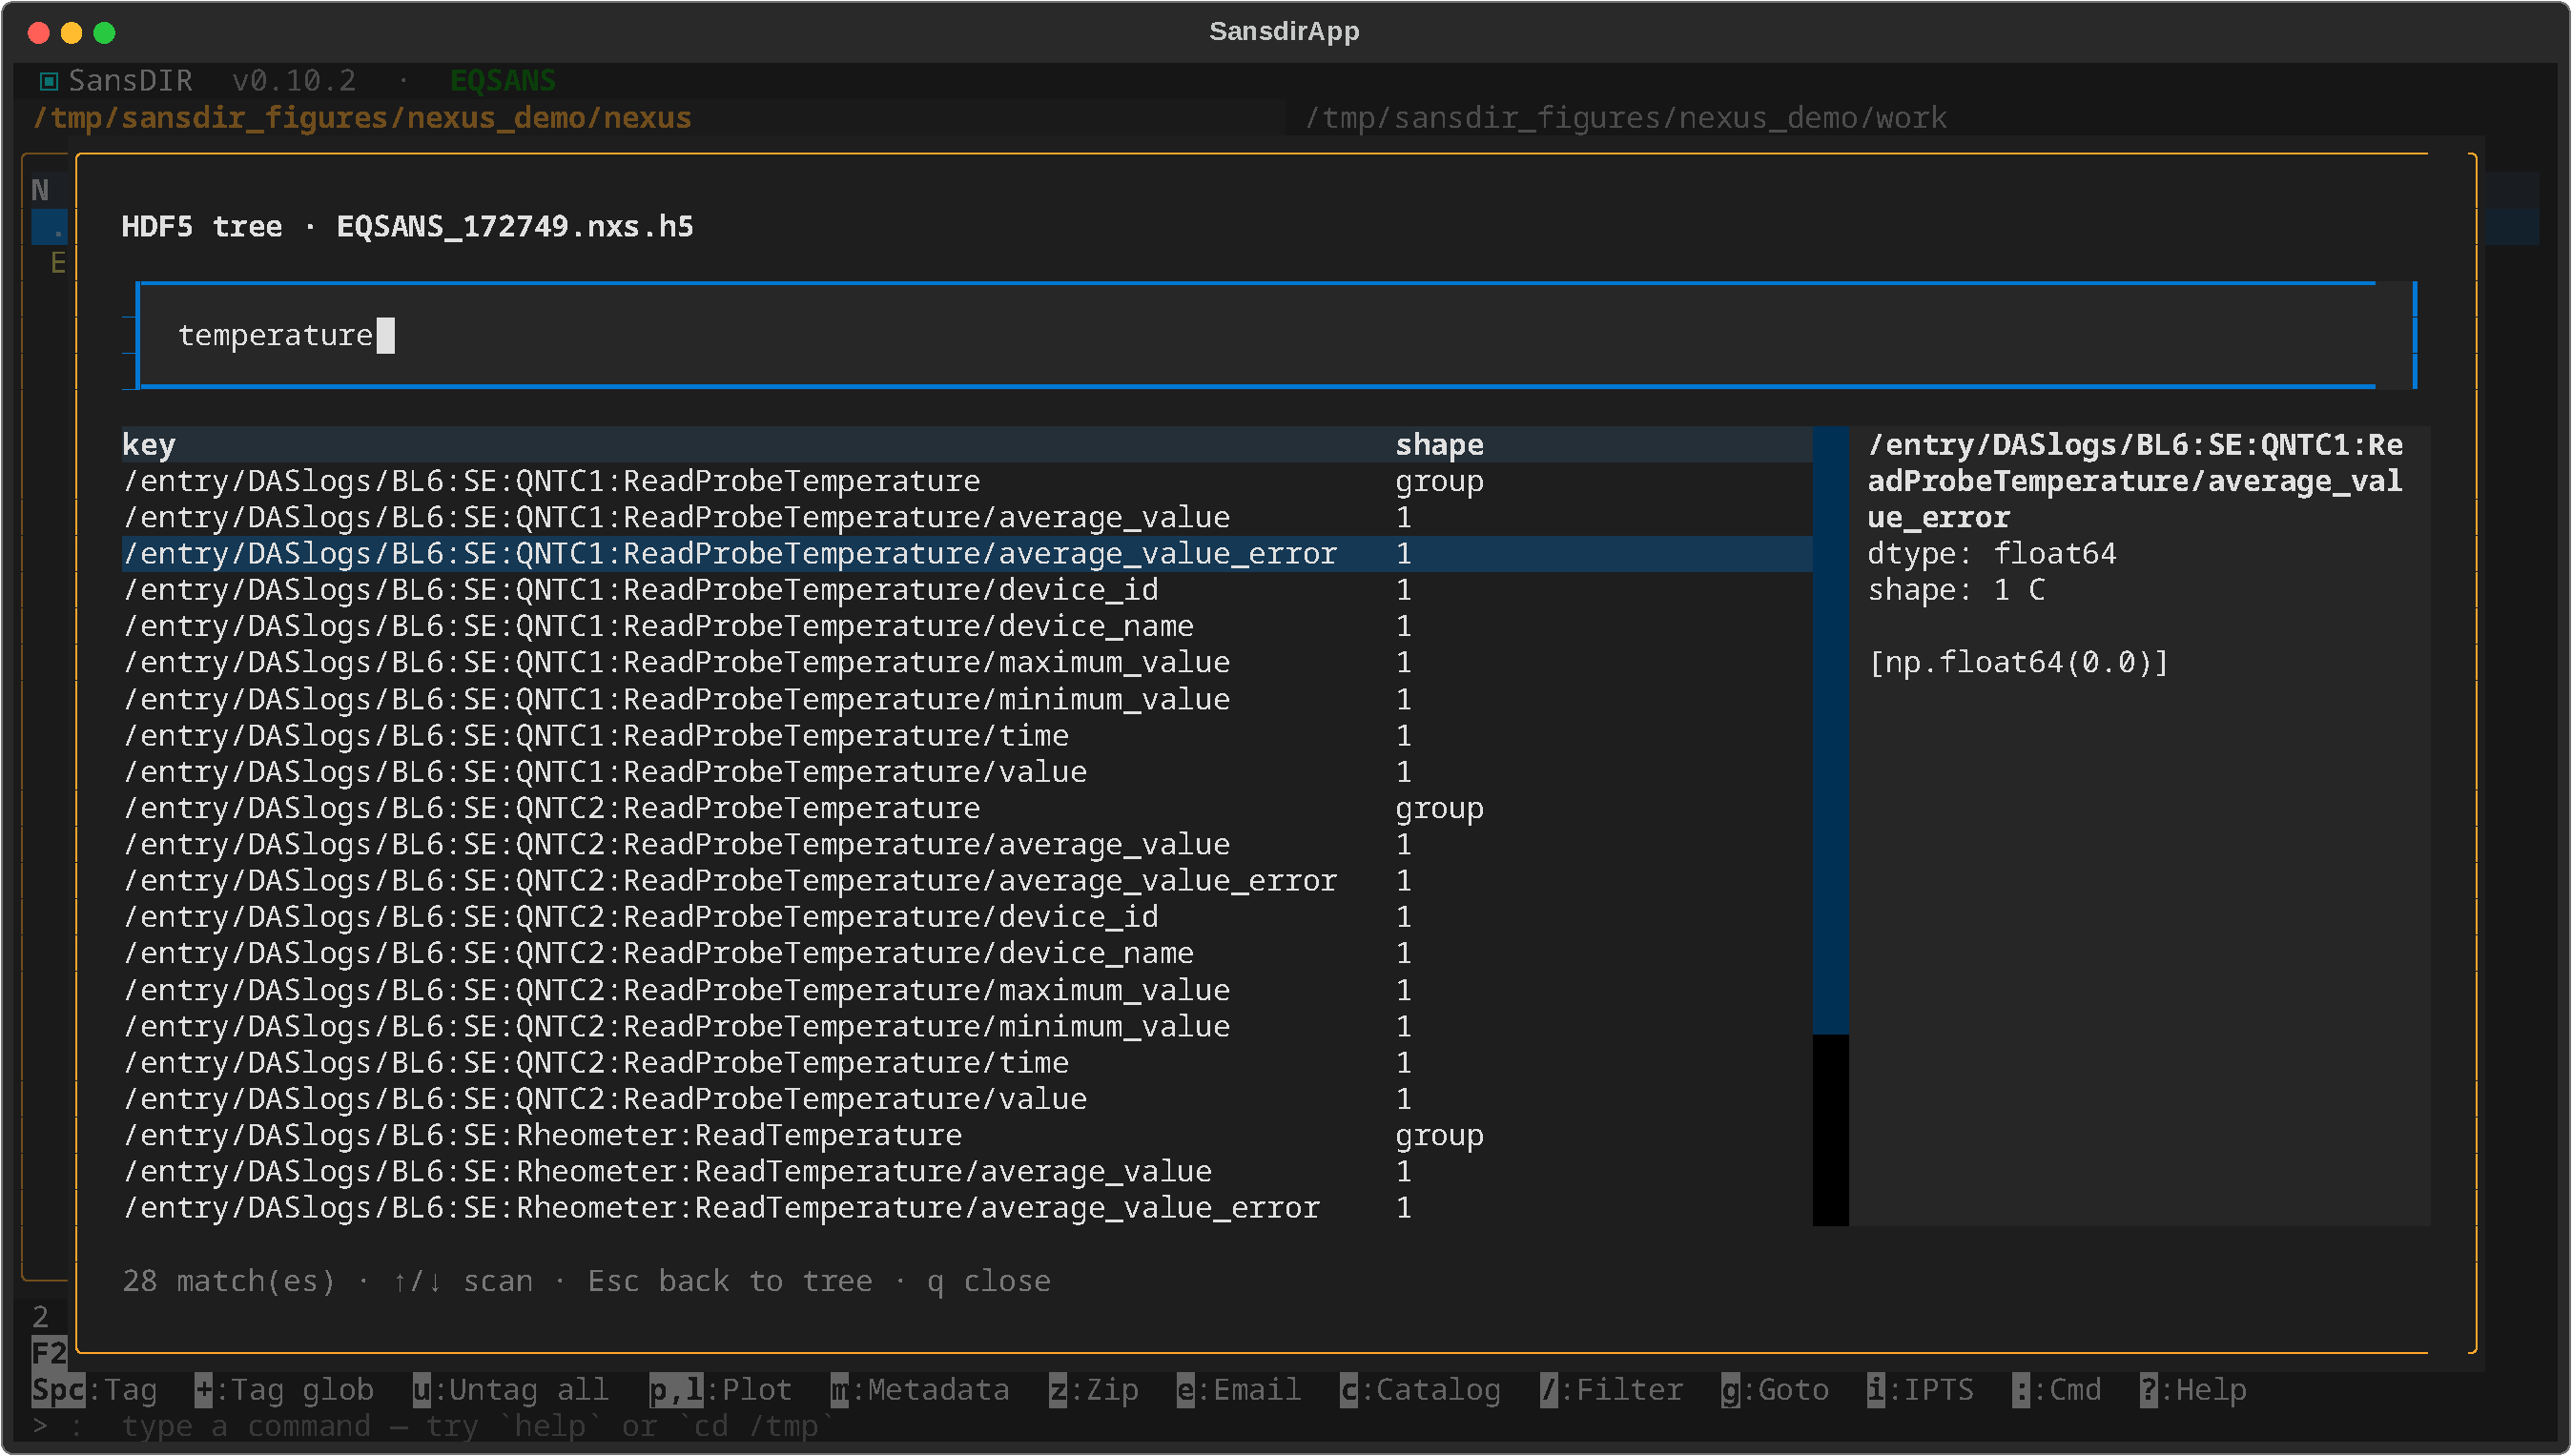
\includegraphics[width=\textwidth]{figures/hdf-search.pdf}
  % Literal "HDF5" rather than \ac{hdf}: the first argument becomes the
  % List of Figures entry, where acro's counter is fresh and would expand to
  % the long form.
  \longcaption{Keyword search in the HDF5 tree browser.}{A substring query
  against a raw EQ-SANS file. The left table lists matching keys with their
  shapes; the right pane shows the highlighted key's dtype, shape, and value
  preview. \key{Esc} returns to the tree view, and a second \key{Esc} closes the
  browser.}
  \label{fig:hdfsearch}
\end{figure}

Two limits keep the search responsive for large files. At most 500 matches are
rendered. If more matches exist, the hint line reports that the results were
truncated. Value previews also take a slice before an array is materialized.
Thus, a preview of an event array with millions of elements reads five values
instead of the full array.

\subsection{BATCH EXTRACTION}

\key{M} extracts selected keys from several files. It first opens a full-screen
key picker. \key{Space} selects a key, and \key{/} searches all keys in the file
with the same method used by the single-file browser. \key{Ctrl+S} returns to
the output form.

Extraction uses a thread pool with eight workers by default, allowing several
files to be read concurrently. The worker count can be changed for the available
filesystem and host.

The key picker accepts either a dataset or a group containing a \texttt{value}
child, as used by the \ac{sns} \ac{das} log convention. Selecting such a group
is the same as selecting \texttt{<group>/value}.

\subsection{OUTPUT MODES}

Two output modes support different questions.

\textbf{Summary mode} produces one row for each input file and reduces
time-series values to their mean. It can answer, for example, what the
temperature was for each of 40 runs. Optional \texttt{\_stdev} and \texttt{\_n}
columns give the spread and sample count for each mean.

\textbf{Per-file mode} produces one table per input file and keeps the full
arrays. It can show, for example, how temperature changed during one run. The
placeholder \texttt{<filename>} in the output template selects this mode, as in
\texttt{<filename>\_temp.csv}. If per-file mode is requested without the
placeholder, the program adds \texttt{<filename>\_} to avoid repeatedly
overwriting one file.

By default, output is written to the working directory of the inactive pane.
The active pane often contains a read-only proposal directory, where writing the
output would cause a permission error.

\subsection{A WORKED EXAMPLE}
\label{sec:metadata-example}

Figures~\ref{fig:metadata-workflow} and~\ref{fig:metadata-workflow-2} show a
complete extraction and plotting example using a real experiment file. The file
is a Mantid-processed workspace from an EQ-SANS measurement with an in-situ
mechanical load frame. The required quantity is the load-cell record, stored in
the \ac{das} log \texttt{BL6:SE:PsyloTech:SGLC}. The goal is to extract this
record as a time series that can be plotted.

\begin{enumerate}
  \item In the active pane, navigate to the file
    (\texttt{IPTS-37828/shared/output/.../*\_processed.nxs}) and point the
    other pane at the directory that should receive the output, here the
    proposal's writable \texttt{shared/} folder.
  \item Press \key{M} to open the key picker on the file's HDF5 tree. Because
    the full \ac{das} log path is not known, press \key{/} and enter the
    fragment \texttt{LC}. Three rows match. Press \key{Space} on
    \texttt{.../SGLC/time} and \texttt{.../SGLC/value}. Both rows are marked,
    and the status line shows \emph{selected: 2 key(s)} (panel~a).
  \item Press \key{Ctrl+S}. The picker folds back into the output form with
    both keys filled in. Per-file mode and the
    \texttt{<filename>\_extracted} template are the defaults. Change the format
    to \ac{csv} and press \key{Ctrl+S} again to run the extraction (panel~b).
  \item The extractor writes
    \texttt{<filename>\_extracted.csv} in the inactive pane's directory. The
    file has two columns, \texttt{time} and \texttt{value}, and 5\,644 rows.
    The pane refreshes and the new file appears (panel~c).
  \item Press \key{Tab} to switch panes, put the cursor on the new \ac{csv},
    and press \key{l}. The generic linear plotter reads the header row for
    axis labels and draws value against time (panel~d). The load increases
    during the first 450~seconds of the run and then releases sharply. Without
    this workflow, the file would need to be exported and opened in a separate
    plotting tool for the same check.
\end{enumerate}

The four panels were captured from the running program and show its actual
fonts, colors, and layout.

\begin{figure}[p]
  \centering
  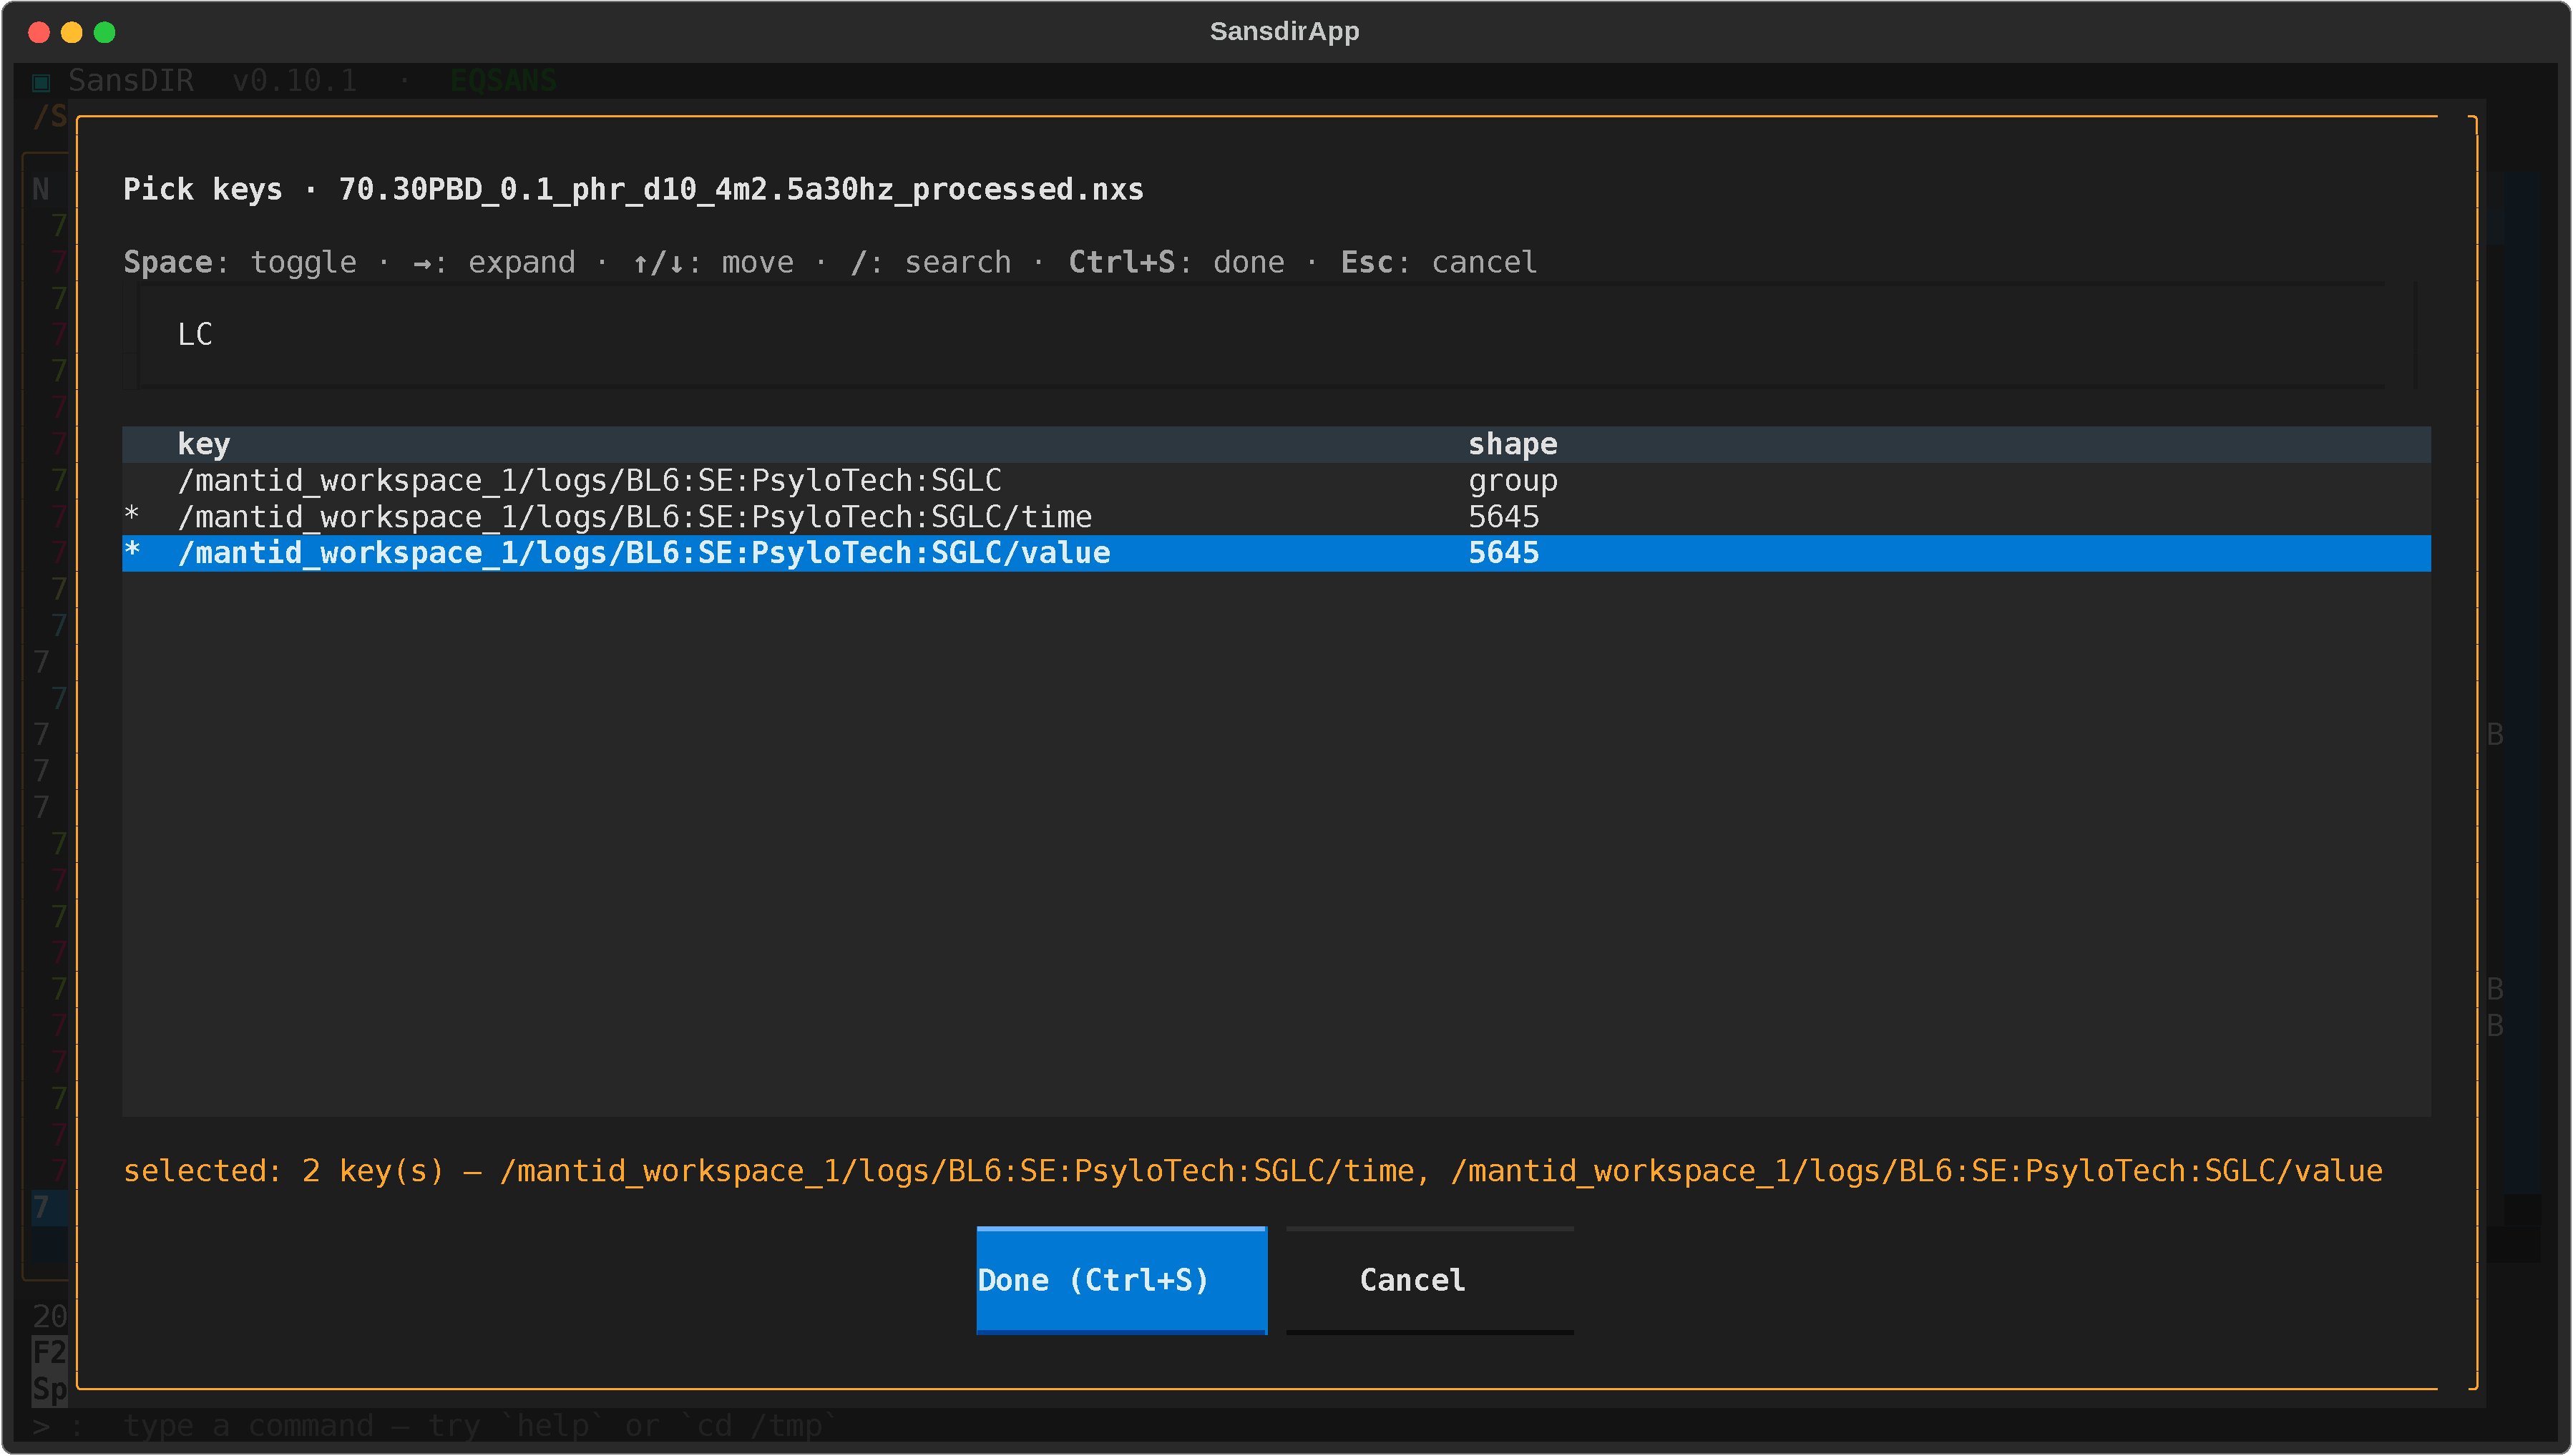
\includegraphics[width=\textwidth]{figures/metadata-workflow-1.pdf}\\[1pt]
  {\small (a) \key{M}, then \key{/}~\texttt{LC}: search and select keys}\\[8pt]
  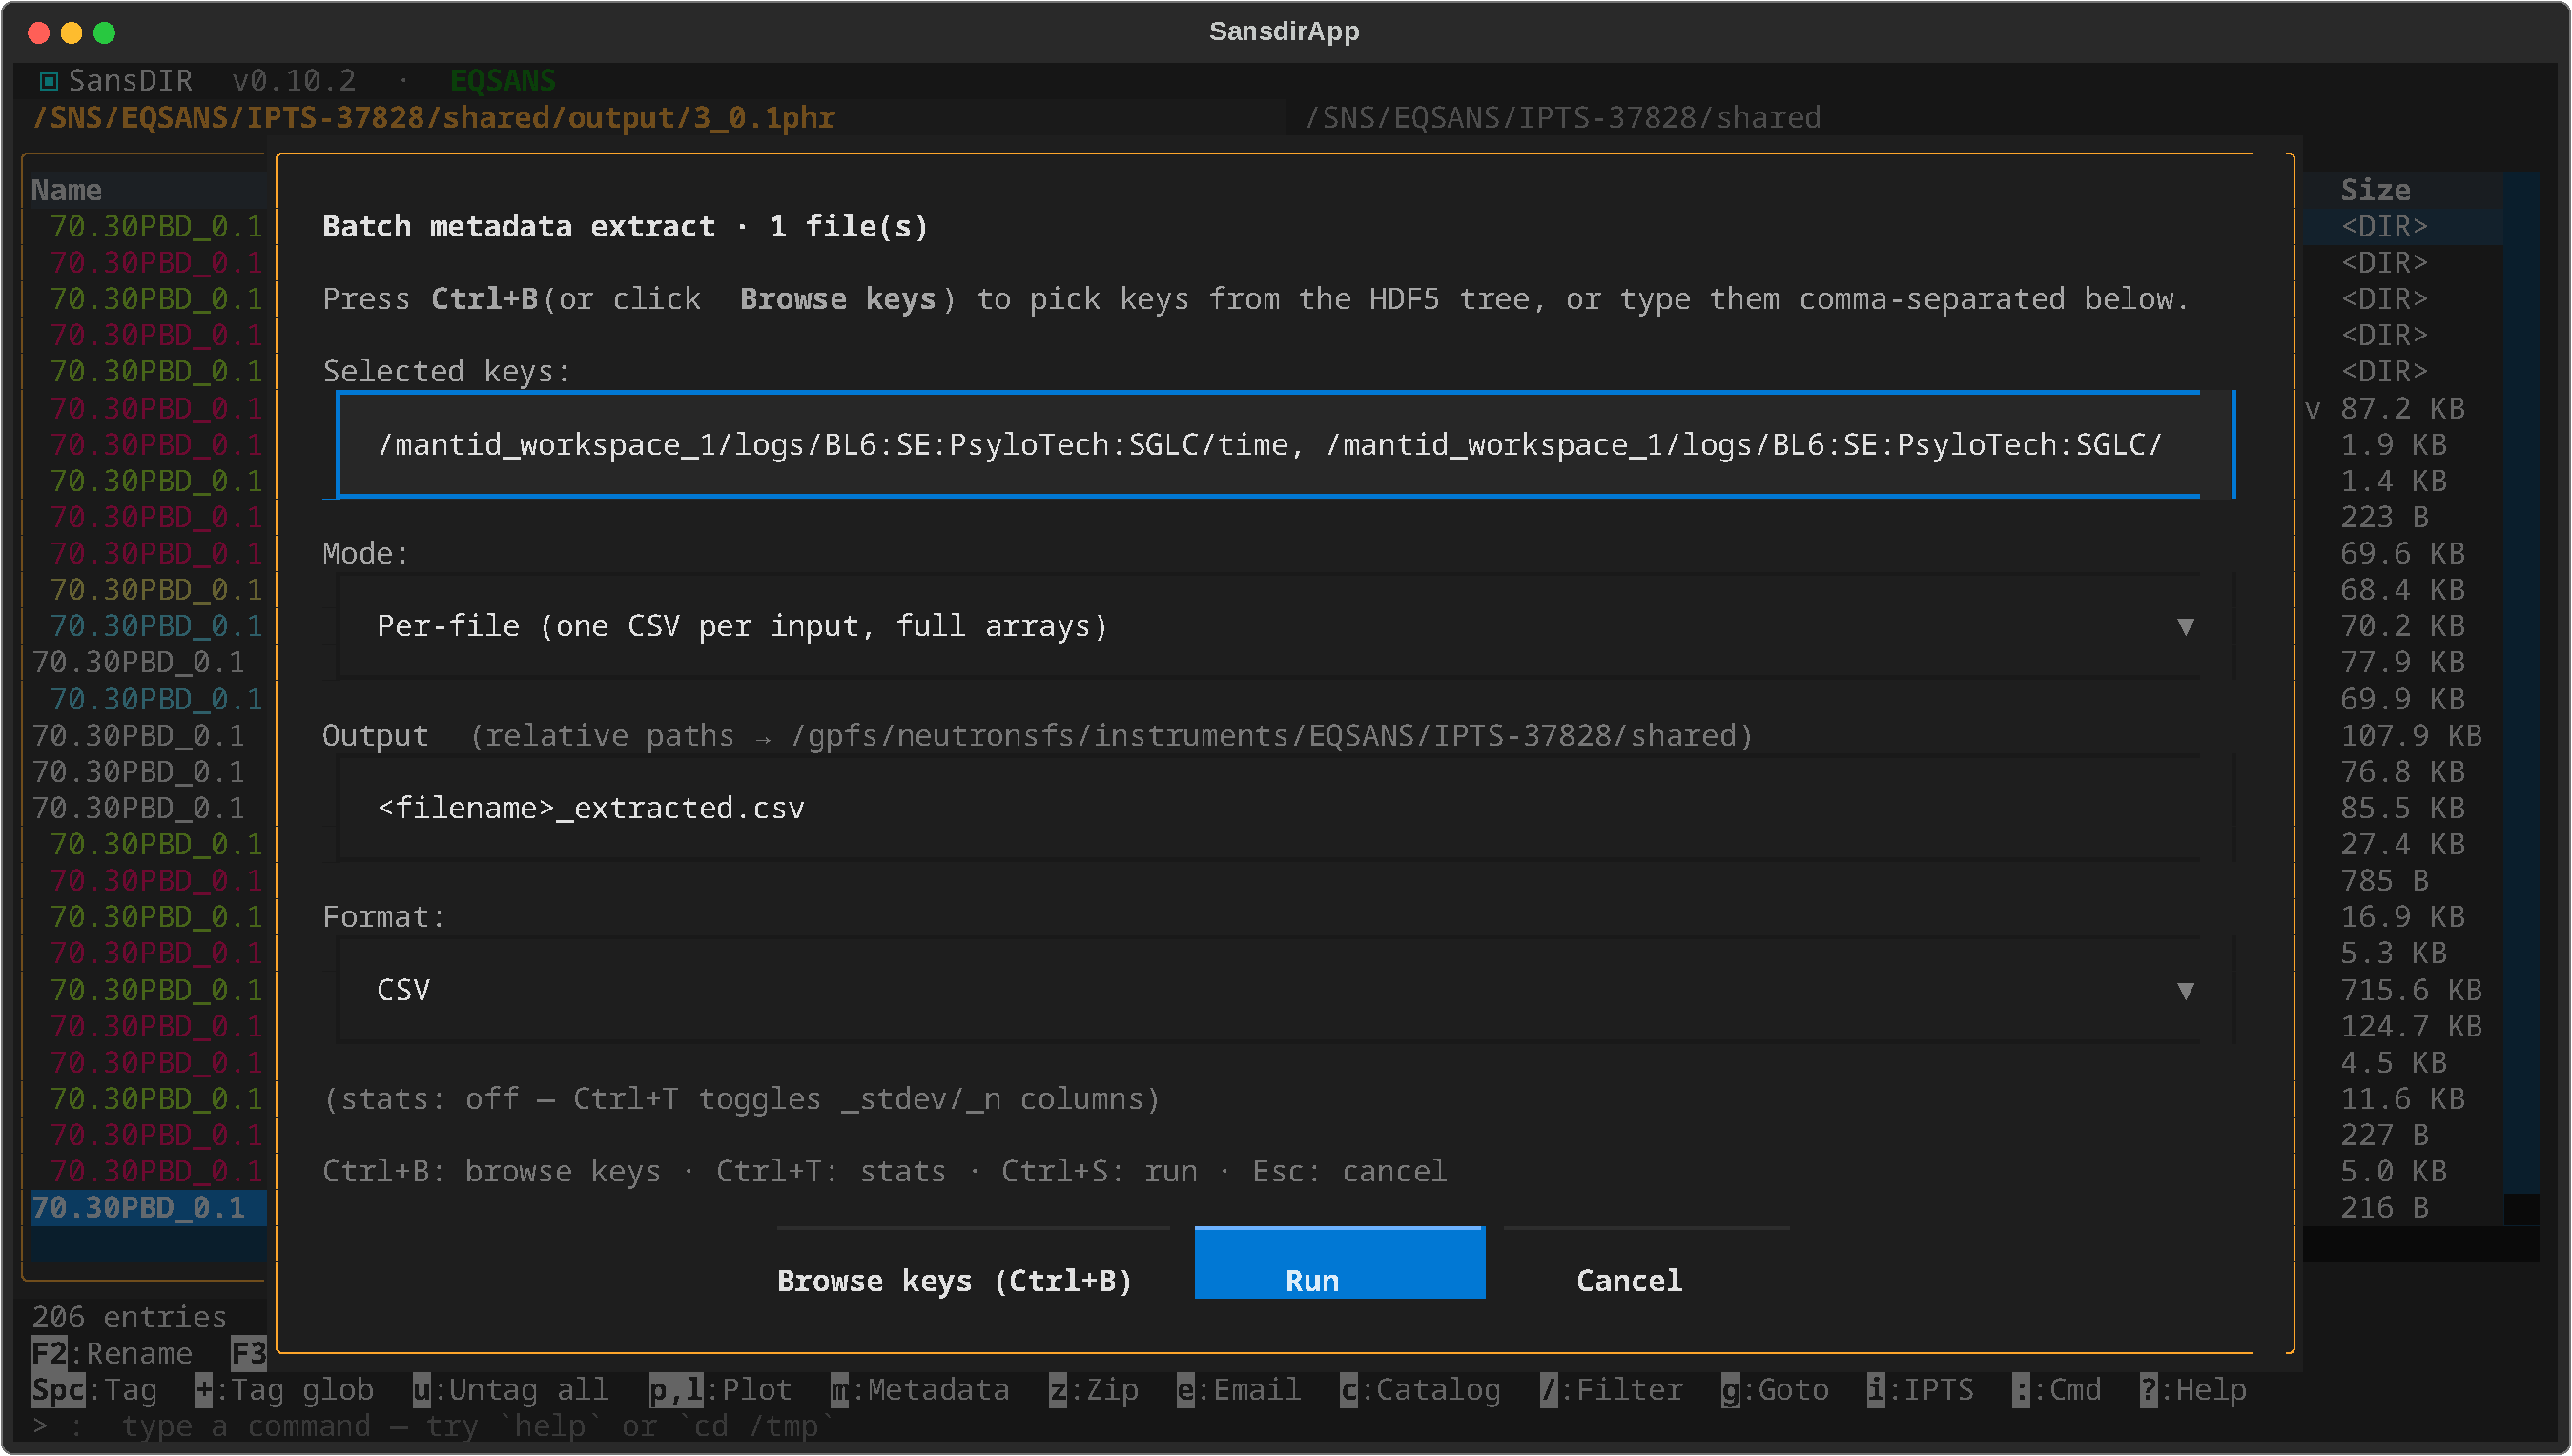
\includegraphics[width=\textwidth]{figures/metadata-workflow-2.pdf}\\[1pt]
  {\small (b) \key{Ctrl+S}: the output form, format set to CSV}
  \longcaption{Batch metadata extraction (1 of 2).}{(a)~The key picker
  after pressing \key{M} and searching for \texttt{LC}: both datasets under
  the \texttt{PsyloTech:SGLC} log are selected. (b)~The output form with the
  chosen keys, per-file mode, and CSV format.}
  \label{fig:metadata-workflow}
\end{figure}

\begin{figure}[p]
  \centering
  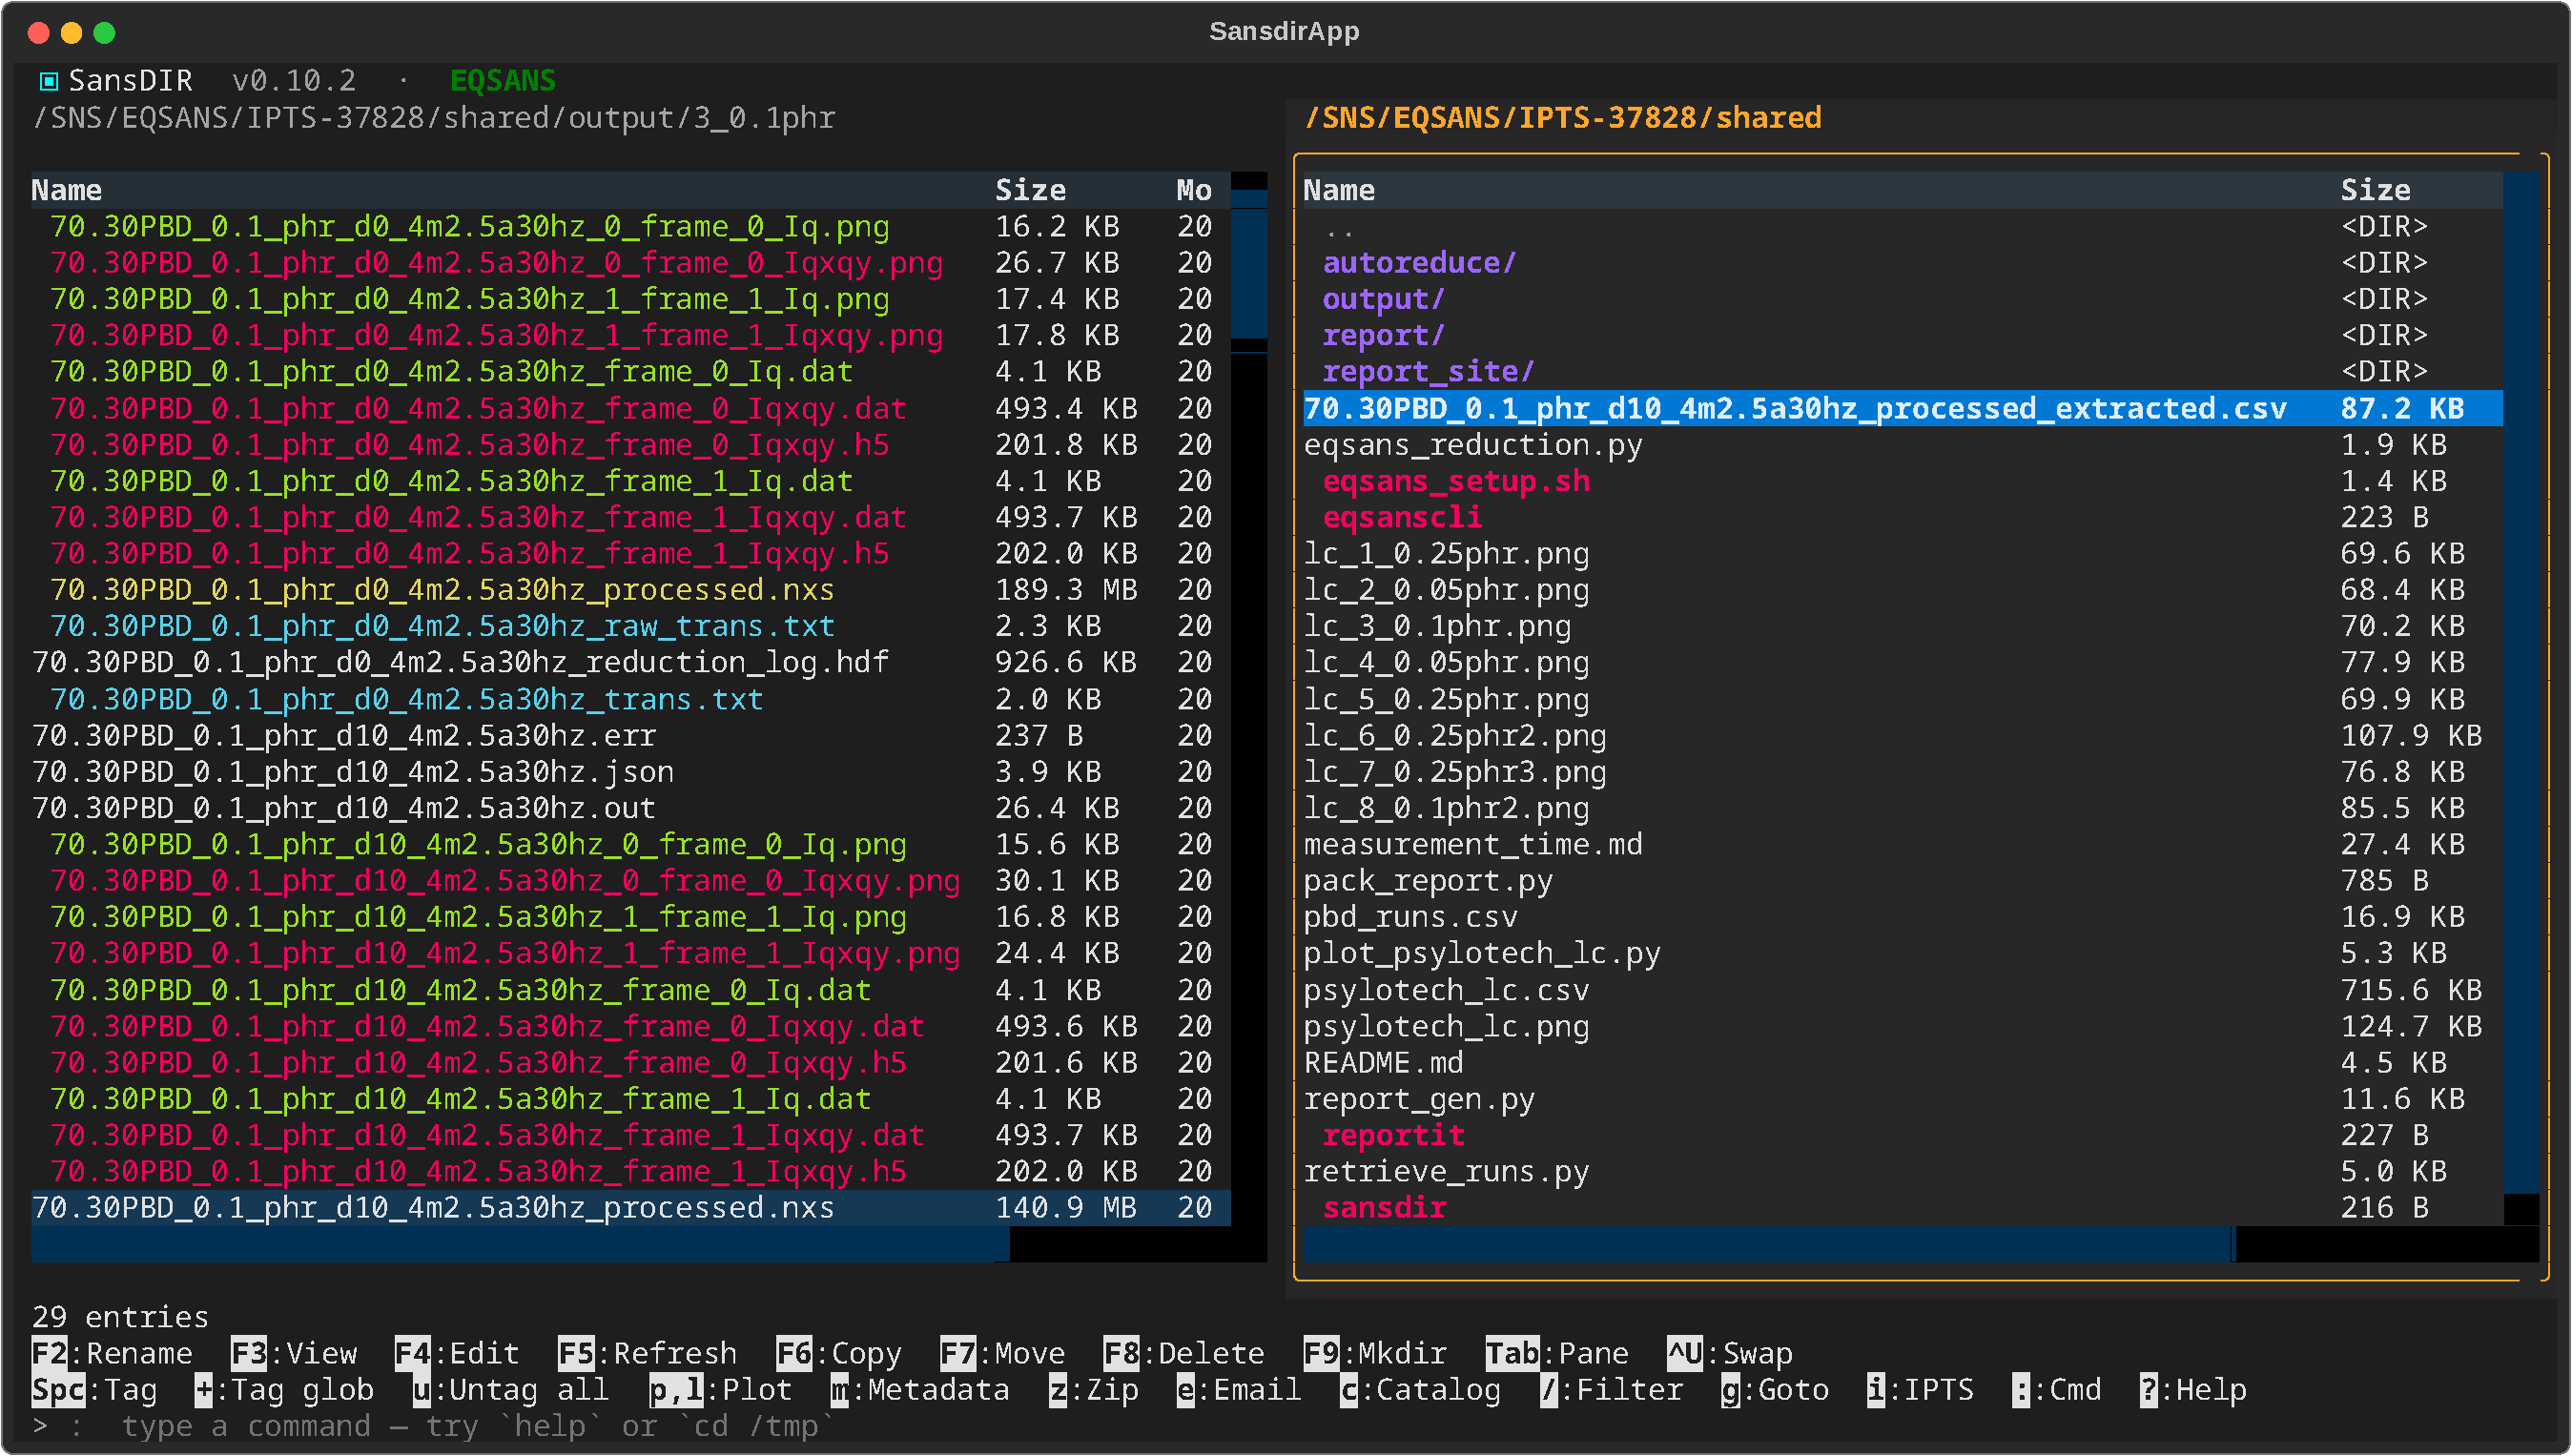
\includegraphics[width=\textwidth]{figures/metadata-workflow-3.pdf}\\[1pt]
  {\small (c) the extracted CSV lands in the other pane}\\[8pt]
  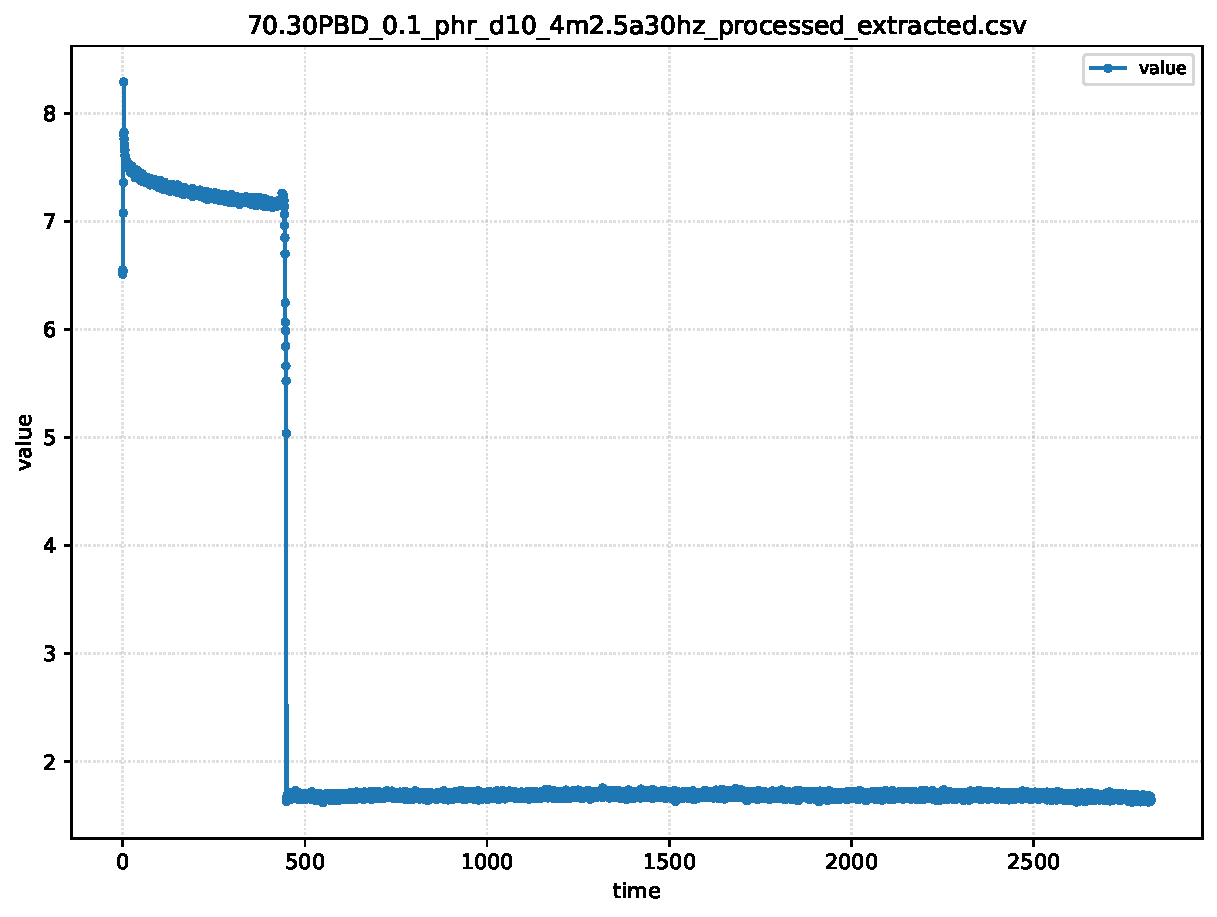
\includegraphics[width=0.62\textwidth]{figures/metadata-workflow-4.pdf}\\[1pt]
  {\small (d) \key{l}: plot of the extracted table}
  \longcaption{Batch metadata extraction (2 of 2).}{(c)~The destination pane
  after the run: the extracted CSV is under the cursor. (d)~The curve
  produced by pressing \key{l} on it---the load-cell trace over the course
  of the run.}
  \label{fig:metadata-workflow-2}
\end{figure}

%%%%%%%%%%%%%%%%%%%%%%%%%%%%%%%%%%%%%%%%%%%%%%%%%%%%%%%%%%%%%%%%%%%%%%%%%%%%%%%
% 8. ONCAT
%%%%%%%%%%%%%%%%%%%%%%%%%%%%%%%%%%%%%%%%%%%%%%%%%%%%%%%%%%%%%%%%%%%%%%%%%%%%%%%
\section{CATALOG INTEGRATION}
\label{sec:oncat}

\subsection{AUTHENTICATION}

OnCat \autocite{oncat} requires an \ac{oauth} bearer token for read-only
endpoints. The client
uses the client-credentials grant to obtain a token and caches it until shortly
before it expires. Credentials are read from the \texttt{[oncat]} configuration
section or the \texttt{ONCAT\_CLIENT\_ID} and \texttt{ONCAT\_CLIENT\_SECRET}
environment variables. Working defaults allow a cluster user to search without
additional configuration. The endpoint is also configurable for use with a
staging instance.

\subsection{SEARCH MODEL AND CACHING}

OnCat does not provide a fuzzy keyword endpoint. Therefore, the client requests
all experiments for the configured instrument, stores the list on disk, and
filters it locally. The filter uses substring matches against the proposal
identifier, title, and member list. The configurable cache \ac{ttl} is 24~hours
by default. The first search requires one server request, while later searches
use the cache and complete in well under a second.

A stale cache may not contain a newly allocated proposal. The \key{r} key in the
browser therefore requests a new list without using the cache.

Two measures keep the browser responsive for large catalogs. A 200~ms quiet
period is applied to the filter input, so the result list is not rebuilt after
every keystroke during fast typing. The browser also renders at most 200 rows
and reports how many additional matches exist.

\subsection{RUN CATALOG PANE}

Selecting a proposal opens its \texttt{shared/} directory in the active pane and
loads its run list in the right pane. \key{c} shows or hides the catalog. In the
catalog, \key{Space} tags runs and the same keys used in the file panes act on
the selection. \key{Enter} or \key{p} plots the raw detector image, \key{m}
opens the \ac{hdf} tree, \key{M} extracts metadata, and \key{K} opens the mask
editor. Thus, the catalog provides another selection view with the same commands
as the file panes.

%%%%%%%%%%%%%%%%%%%%%%%%%%%%%%%%%%%%%%%%%%%%%%%%%%%%%%%%%%%%%%%%%%%%%%%%%%%%%%%
% 9. MASK
%%%%%%%%%%%%%%%%%%%%%%%%%%%%%%%%%%%%%%%%%%%%%%%%%%%%%%%%%%%%%%%%%%%%%%%%%%%%%%%
\section{DETECTOR MASK CREATION}
\label{sec:mask}

\subsection{ARCHITECTURAL CONSTRAINTS}

Detector masking produces an input to reduction instead of displaying reduction
output. Its implementation follows three constraints:

\begin{itemize}
  \item \textbf{No Mantid import in the main process.} Mask drawing and array
    creation use Python, \texttt{numpy}, and \texttt{h5py}. At save time, a
    standalone driver imports Mantid inside an external \texttt{drtsans}
    subprocess. The \ac{tui} process does not import Mantid.
  \item \textbf{EQ-SANS geometry is isolated.} Detector shape, tube reordering,
    and the 48-bank mapping are kept in the detector and bank/tube modules. When
    the source NeXus file provides a pixel-identifier array, the program uses it
    to connect the displayed pixels to detector identifiers.
  \item \textbf{Pixel ordering is defined in exactly one place.} One module
    establishes that the flattened mask array and pixel identifier array are
    aligned element by element. The output writers use this ordering instead of
    calculating it again.
\end{itemize}

The mask uses the Mantid convention: 1 is a masked pixel and 0 is a retained
pixel. Therefore, \texttt{MaskDetectors} excludes the cells selected by the
user. One flag inverts the final mask.

\subsection{INTERACTIVE EDITOR}

From a file pane or the run catalog, \key{K} opens a matplotlib window containing
the detector heat map of the selected file. The user draws mask shapes on this
image.

The cell aspect ratio is $1/1.3$ to account for the EQ-SANS detector tube pitch
of about 5.2~mm and pixel pitch of about 3.9~mm. Without this correction, an
ellipse that appears circular on the screen would not be circular on the
detector. The canvas also extends several cells beyond the detector boundary,
which is marked by a faint dotted line. A selection can then begin outside the
active area. Otherwise, masking the outermost row would require the first click
to be exactly on pixel zero.

Table~\ref{tab:maskkeys} lists the editor's controls.

\begin{table}[ht]
  \centering
  \caption{Interactive mask editor controls}
  \label{tab:maskkeys}
  \small
  \begin{tabular}{l p{0.72\textwidth}}
    \toprule
    Key & Action \\
    \midrule
    \key{r} & Rectangle draw mode \\
    \key{e} & Ellipse draw mode \\
    \key{v} & Edit mode: click to select a shape, drag to move it, \key{Delete}
      to remove it \\
    \key{k} & Open the bank and tube specification dialog \\
    \key{z} & Undo \\
    \key{i} & Invert the mask \\
    \key{s} & Save, through a file chooser \\
    \key{Esc} & Quit without saving \\
    \bottomrule
  \end{tabular}
\end{table}

The bank and tube dialog accepts a compact notation. For example,
\texttt{b3} selects a complete bank, \texttt{t50} selects a tube, and
\texttt{b5-7 t10-15} selects mixed ranges. This is useful for strip masks that
are difficult to draw by hand. The resulting rectangles are ordinary shapes and
are stored in the mask log like other shapes.

Two changes improved the response of the editor. When a shape is moved, the
static canvas is saved at mouse-down and only the moving area is drawn for each
motion event. The full heat map is not redrawn. Also, bank and tube input uses a
dialog instead of an inline matplotlib text widget. The inline widget redraws
after every keystroke, which produces visible input delay on a logarithmically
scaled $256\times192$ image.

As the pointer moves, a cursor readout shows \texttt{tube}, \texttt{pixel},
\texttt{counts}, \texttt{bank}, and the tube index within its bank. These values
help the user convert a feature in the image into a bank and tube specification.

\subsection{COMMAND-LINE MASK CREATION}

The same operations are available from the command line. Shapes are specified in
pixel coordinates, and each option can be repeated:

\begin{lstlisting}[language=shellsession]
sansdir mask /SNS/EQSANS/IPTS-XXXXX/nexus/EQSANS_172749.nxs.h5 \
  --circle 96,128,12 \
  --rect 0,0,15,15   --rect 176,0,191,15 \
  --rect 0,240,15,255 --rect 176,240,191,255 \
  --output beam_stop.nxs
\end{lstlisting}

The available shapes are \texttt{--rect X0,Y0,X1,Y1}, \texttt{--ellipse
XC,YC,RX,RY}, \texttt{--circle XC,YC,R}, and \texttt{--polygon
X1,Y1,X2,Y2,...} with at least three vertices. Each output has a sidecar
\ac{json} log. The \texttt{--shapes-json} option reads this log, allowing a mask
created interactively to be applied to other runs in a script.

\subsection{OUTPUT FORMATS AND REDUCTION COMPATIBILITY}

The program supports three output formats: a Mantid \texttt{SaveMask} \ac{xml}
file, a NeXus file, and a \texttt{numpy} array with a metadata sidecar.

The NeXus output requires an additional step. A mask used by the
\texttt{drtsans} reduction pipeline must contain per-detector mask flags in the
instrument parameter map read by the pipeline. Mantid is used to write this
structure. During saving, the program calls the cluster's \texttt{drtsans}
wrapper and runs a load--mask--save sequence on the source file. If Mantid is not
available, a pure-\texttt{numpy} writer produces a file for visualization only.
The \ac{tui} briefly identifies this as a legacy save, while the \ac{cli} does
not give a prominent fallback warning. This file can be inspected but does not
change a reduction.

The visualization file follows the convention of existing EQ-SANS beam-stop
files. Each \emph{unmasked} detector contains one synthetic event, while masked
detectors contain no events. Therefore, a mask opened with \key{p} shows the
masked area in grey, like a beam stop. The mask builder continues to use
Mantid's ``1 means masked'' convention internally; only the file encoding is
inverted.

%%%%%%%%%%%%%%%%%%%%%%%%%%%%%%%%%%%%%%%%%%%%%%%%%%%%%%%%%%%%%%%%%%%%%%%%%%%%%%%
% 10. CLI
%%%%%%%%%%%%%%%%%%%%%%%%%%%%%%%%%%%%%%%%%%%%%%%%%%%%%%%%%%%%%%%%%%%%%%%%%%%%%%%
\section{NON-INTERACTIVE COMMAND-LINE INTERFACE}
\label{sec:cli}

Several operations are available without the \ac{tui} for scripts and batch
jobs. The Click \ac{cli} is a separate entry path, but it calls the same service
functions used by the interactive commands.

\subsection{LAUNCHING THE INTERFACE}

\begin{lstlisting}[language=shellsession]
sansdir                                # TUI in the current directory
sansdir /SNS/EQSANS/IPTS-12345/shared  # TUI rooted at a directory
\end{lstlisting}

A path given without a subcommand is interpreted as \texttt{sansdir tui PATH}.
Thus, the subcommand name can be omitted for normal interactive use.

\subsection{BATCH METADATA EXTRACTION}

\begin{lstlisting}[language=shellsession]
# Summary table: one row per file, time series reduced to means.
sansdir extract \
  -k /entry/DASlogs/temperature/value \
  -k /entry/duration \
  --out summary.tsv \
  /SNS/EQSANS/IPTS-12345/nexus/EQSANS_*.nxs.h5

# Per-file tables: each input gets its own CSV with full arrays.
sansdir extract \
  -k /entry/DASlogs/temperature/time \
  -k /entry/DASlogs/temperature/value \
  --out '<filename>_temp.csv' \
  EQSANS_172749.nxs.h5 EQSANS_172750.nxs.h5

# Add spread and sample-count columns (summary mode only).
sansdir extract --with-stats -k /entry/DASlogs/temperature/value *.nxs.h5
\end{lstlisting}

The options are \texttt{-k/--keys} (repeatable and required),
\texttt{-o/--out}, \texttt{--format} with the values \texttt{tsv},
\texttt{csv}, or \texttt{columns}, \texttt{--with-stats}, and
\texttt{--workers} for the thread-pool size. Each written path is printed on a
separate line, allowing the command to be used in a shell pipeline.

\subsection{MASK CREATION}

Section~\ref{sec:mask} describes the \texttt{mask} subcommand. Its options
are \texttt{--rect}, \texttt{--ellipse}, \texttt{--circle}, \texttt{--polygon},
\texttt{--shapes-json}, \texttt{--inverse}, \texttt{--output}, and
\texttt{--format} with values \texttt{nxs}, \texttt{xml}, or \texttt{npy}. When
complete, it reports the output path, masked pixel count as a number and
percentage, and sidecar log path.

%%%%%%%%%%%%%%%%%%%%%%%%%%%%%%%%%%%%%%%%%%%%%%%%%%%%%%%%%%%%%%%%%%%%%%%%%%%%%%%
% 11. CONFIGURATION
%%%%%%%%%%%%%%%%%%%%%%%%%%%%%%%%%%%%%%%%%%%%%%%%%%%%%%%%%%%%%%%%%%%%%%%%%%%%%%%
\section{CONFIGURATION}
\label{sec:config}

Configuration is read from \texttt{\hme/.config/sansdir/config.toml} or from the
path given by \texttt{\$SANSDIR\_CONFIG}. All sections and keys are optional, and
the program can run without a configuration file.

\begin{lstlisting}
[ui]
theme = "monokai"       # any Textual theme name
colorbar_mode = "shared"   # tiled 2-D scale: "shared" or "independent"

[keys]
"ctrl+y" = "view.toggle_hidden"   # bind a key to a compatible command
f5 = "ui.move_tagged"             # replace the default F5 action

[oncat]
default_instrument = "EQSANS"
cache_ttl_seconds  = 86400

[instrument]
default     = "EQSANS"   # "" falls back to [oncat].default_instrument
auto_detect = true       # a /SNS/USANS/... launch path overrides `default`

[usans]
pixi_manifest     = "/usr/local/pixi/usansred"
reduce_command    = ""   # explicit override for the engine argv
data_dir_template = "/SNS/USANS/{ipts}/shared/autoreduce"
logbin            = true
thickness_cm      = 0.1
short_name_copy   = true   # also write UN_*_bsub.txt aliases

[mail]
command = "mail"                  # or "mutt"
default_subject = "[sansdir] data"
\end{lstlisting}

The loader handles several invalid settings without stopping the program. An
unknown theme name is replaced by the default and reported to the user. A key
binding that names an unknown command is removed and also reported. A malformed
TOML file or an invalid value type can still stop startup and must be corrected
in the configuration file.

A custom key binding is most suitable for a command that requires no arguments.
The configuration override stores a key and command name but does not add the
argument resolver used by some built-in bindings.

The theme can also be changed during a session with
\texttt{:theme <name>}. Entering \texttt{:theme} without an argument lists the
available themes.

%%%%%%%%%%%%%%%%%%%%%%%%%%%%%%%%%%%%%%%%%%%%%%%%%%%%%%%%%%%%%%%%%%%%%%%%%%%%%%%
% 11b. USANS REDUCTION
%%%%%%%%%%%%%%%%%%%%%%%%%%%%%%%%%%%%%%%%%%%%%%%%%%%%%%%%%%%%%%%%%%%%%%%%%%%%%%%
\section{USANS REDUCTION}
\label{sec:usans}

\Ac{usans} uses many operations that were already available in the program: the
proposal catalog, file manager, one-dimensional plotting, and editor. It adds a
short reduction workflow and a desmearing step. The instrument team's
\texttt{usansred} package performs the reduction. The desmearing operation uses
the truncated Abel inversion of Huang \autocite{huang2026abel}. These operations
are included through an \emph{instrument mode} and a small, self-contained
module instead of a separate application.

\subsection{INSTRUMENT MODE}

The mode is either \ac{sans} or \ac{usans}. It is resolved once at launch, using
path detection first, then \texttt{[instrument].default}, and finally
\texttt{[oncat].default\_instrument}. A launch path containing
\texttt{usans} selects \ac{usans}. This includes
\texttt{/SNS/USANS/IPTS-\textit{N}} and a user's own scratch directories. Path
detection has priority over the configuration file because the path gives the
current working context. The command \texttt{instrument.set}, entered as
\texttt{:instrument usans}, can change the mode during a session.

The mode controls four items: the instrument queried by the proposal browser,
the columns shown in the run catalog, the action of \key{Enter} on a catalog
row, and whether the \key{r} and \key{d} bindings are active. \Ac{usans} has no moveable
detector and uses a fixed incident wavelength, so the distance and wavelength
columns would contain only constants and are omitted. The title bar shows the
mode, and the reduction and desmearing actions appear in the key hint bar in
\ac{usans} mode.

The mode changes \emph{bindings}, not command registrations. The \ac{usans}
commands are registered in both modes, so \texttt{:usans-reduce} works even if
the user did not switch modes; only the key bindings are hidden. The live help
overlay and hint bar request the key map for the current instrument mode.
Calling \texttt{default\_keymap()} without a mode still returns the original
\ac{sans} map for backward compatibility.

\subsection{THE SETUP TABLE}

The reduction engine reads a small \ac{csv} table with one row per sample. Each
row contains a flag that distinguishes the empty-cell background from the
samples, a name used as the output filename stem, a first run number, a scan
count, a thickness, and optional runs to exclude. The program generates a draft
from the proposal run list. The user then reviews and corrects it with \key{F4},
using the same editor as for other files. A separate table editor is not needed.

During generation, consecutive runs with the same title are grouped into blocks.
The block whose title identifies an empty cell or banjo is selected as the
background. The scan count requires additional checking. A block of $N$
consecutive runs contains $(N-1)$ analyzer rocking-curve scans and one
transmission run, while the engine reads only the rocking-curve files. The value
of $N$ depends on the experiment settings. Therefore, using the catalog run
count would make the engine look for an input file that does not exist for the
transmission run. Instead, the program counts the runs that have rocking-curve
files on disk. This works for different block sizes without additional
configuration. A gap inside a block is recorded in the exclude column of the
\ac{csv}.

Some cases still require review. If a measurement was stopped and restarted
under one title, it can produce an oversized block in which only the last few
runs are usable. The generator keeps the last window of the modal size and flags
the block. A companion notes file records every such choice: narrowed blocks,
unusual sizes, blocks with no reducible runs, removed transmission runs, and the
selected background. The generated table is a first draft. The notes provide
the information needed to review it.

\subsection{INVOKING THE ENGINE}

The instrument team's \texttt{usansred} package contains the reduction
mathematics and is deployed on the cluster as a pixi environment. The program
locates its console script and runs it as a subprocess. It does not reimplement
the physics, and no \texttt{usansred} code is copied into this code base. The
caller also handles two deployment conditions.

First, the console script can inherit the user's \texttt{\textasciitilde
/.local} site packages. On the analysis nodes, an old \texttt{pandas} package in
this location causes the script to stop. Therefore, each invocation disables
user site packages and clears \texttt{PYTHONPATH}.

Second, the engine locates each run relative to the directory containing the
setup \ac{csv}, not relative to the working directory. The reviewed table is
normally in the user's folder, while the preprocessed data are in the proposal's
autoreduce directory. The program must not write to this instrument data
directory, which is also often read-only. It instead creates a temporary
directory containing symbolic links to the data, copies the table there, and
runs the engine in that directory. It does not modify anything below the
instrument data root.

\subsection{ONE KEY}

One binding provides both operations. If the cursor is on a setup table,
\key{r} reduces it. If the cursor is not on a table, the program offers to build
one for the proposal identified by the current path. It fetches the run list,
shows the catalog in the other pane, writes the table, and leaves the cursor on
the new file.

The program stops after writing the draft and does not begin reduction. The user
can review the table and the choices recorded in the notes before pressing
\key{r} again. A table that can be parsed but fails validation is not regenerated.
For example, it may contain two backgrounds or a zero scan count. In this case,
the table may include real user corrections, so regeneration could discard
them. The program reports the problem and directs the user to \key{F4}.

The reduced output is ordinary two- or three-column text and is handled by the
existing plotting path. Only a filename rule was added to the classifier. The
rule uses the filename rather than the column count, so a sample name containing
\texttt{trans} is not incorrectly sent to the transmission plotter.

The engine gives the final curve the suffix
\texttt{\_background\_subtracted.txt}. After each reduction, the program also
writes a shorter \texttt{\_bsub.txt} name. It keeps the original so that the
engine's summary spreadsheet and other tools that expect the standard name
continue to work. The shorter file is a copy, not a symbolic link, and is
controlled by \texttt{[usans].short\_name\_copy}.

\subsection{A WORKED EXAMPLE}
\label{sec:usans-example}

Figures~\ref{fig:usans-workflow} and~\ref{fig:usans-workflow-2} show the complete
workflow for a real proposal (IPTS-37679). It starts with an empty working folder
and ends with reduced curves, using the \key{r} key and the related prompts.

\begin{enumerate}
  \item Open the program in a writable working folder under the proposal path.
    The \texttt{/SNS/USANS} prefix selects \ac{usans} mode automatically.
  \item Press \key{r}. The folder holds no setup table yet, so the program
    offers to build one for the \ac{ipts} named by the path
    (panel~a). Confirm with \key{y}.
  \item The run list is fetched from the catalog and displayed in the other
    pane, and a prompt asks for the first run of the experiment---here
    49434 (panel~b). Blocks recorded before that run, including beam-cycle
    alignment and test scans, are recorded in the notes but omitted from the
    table.
  \item The program writes \texttt{IPTS-37679\_setup.csv} and its companion
    \texttt{NOTE.md}, leaves the cursor on the table, and previews its content
    in the other pane (panel~c). In this case, it contains one background and
    23 sample blocks. The user checks the selected background and block sizes
    against the NOTE and edits the table with \key{F4} if needed.
  \item Press \key{r} again, now on the table. The data directory defaults to
    the proposal's \texttt{autoreduce} folder and the output directory to
    \texttt{output/} beside the table; accepting both runs the engine over
    every block. This takes seconds because it reads the preprocessed per-run
    ASCII files. On completion, the program offers to show the output folder in
    the other pane (panel~d), where each sample now has its
    \texttt{UN\_*\_det\_1\_*} curve family. \key{p} plots any of them, and
    \key{d} desmears (Section~\ref{sec:desmear}).
\end{enumerate}

\begin{figure}[p]
  \centering
  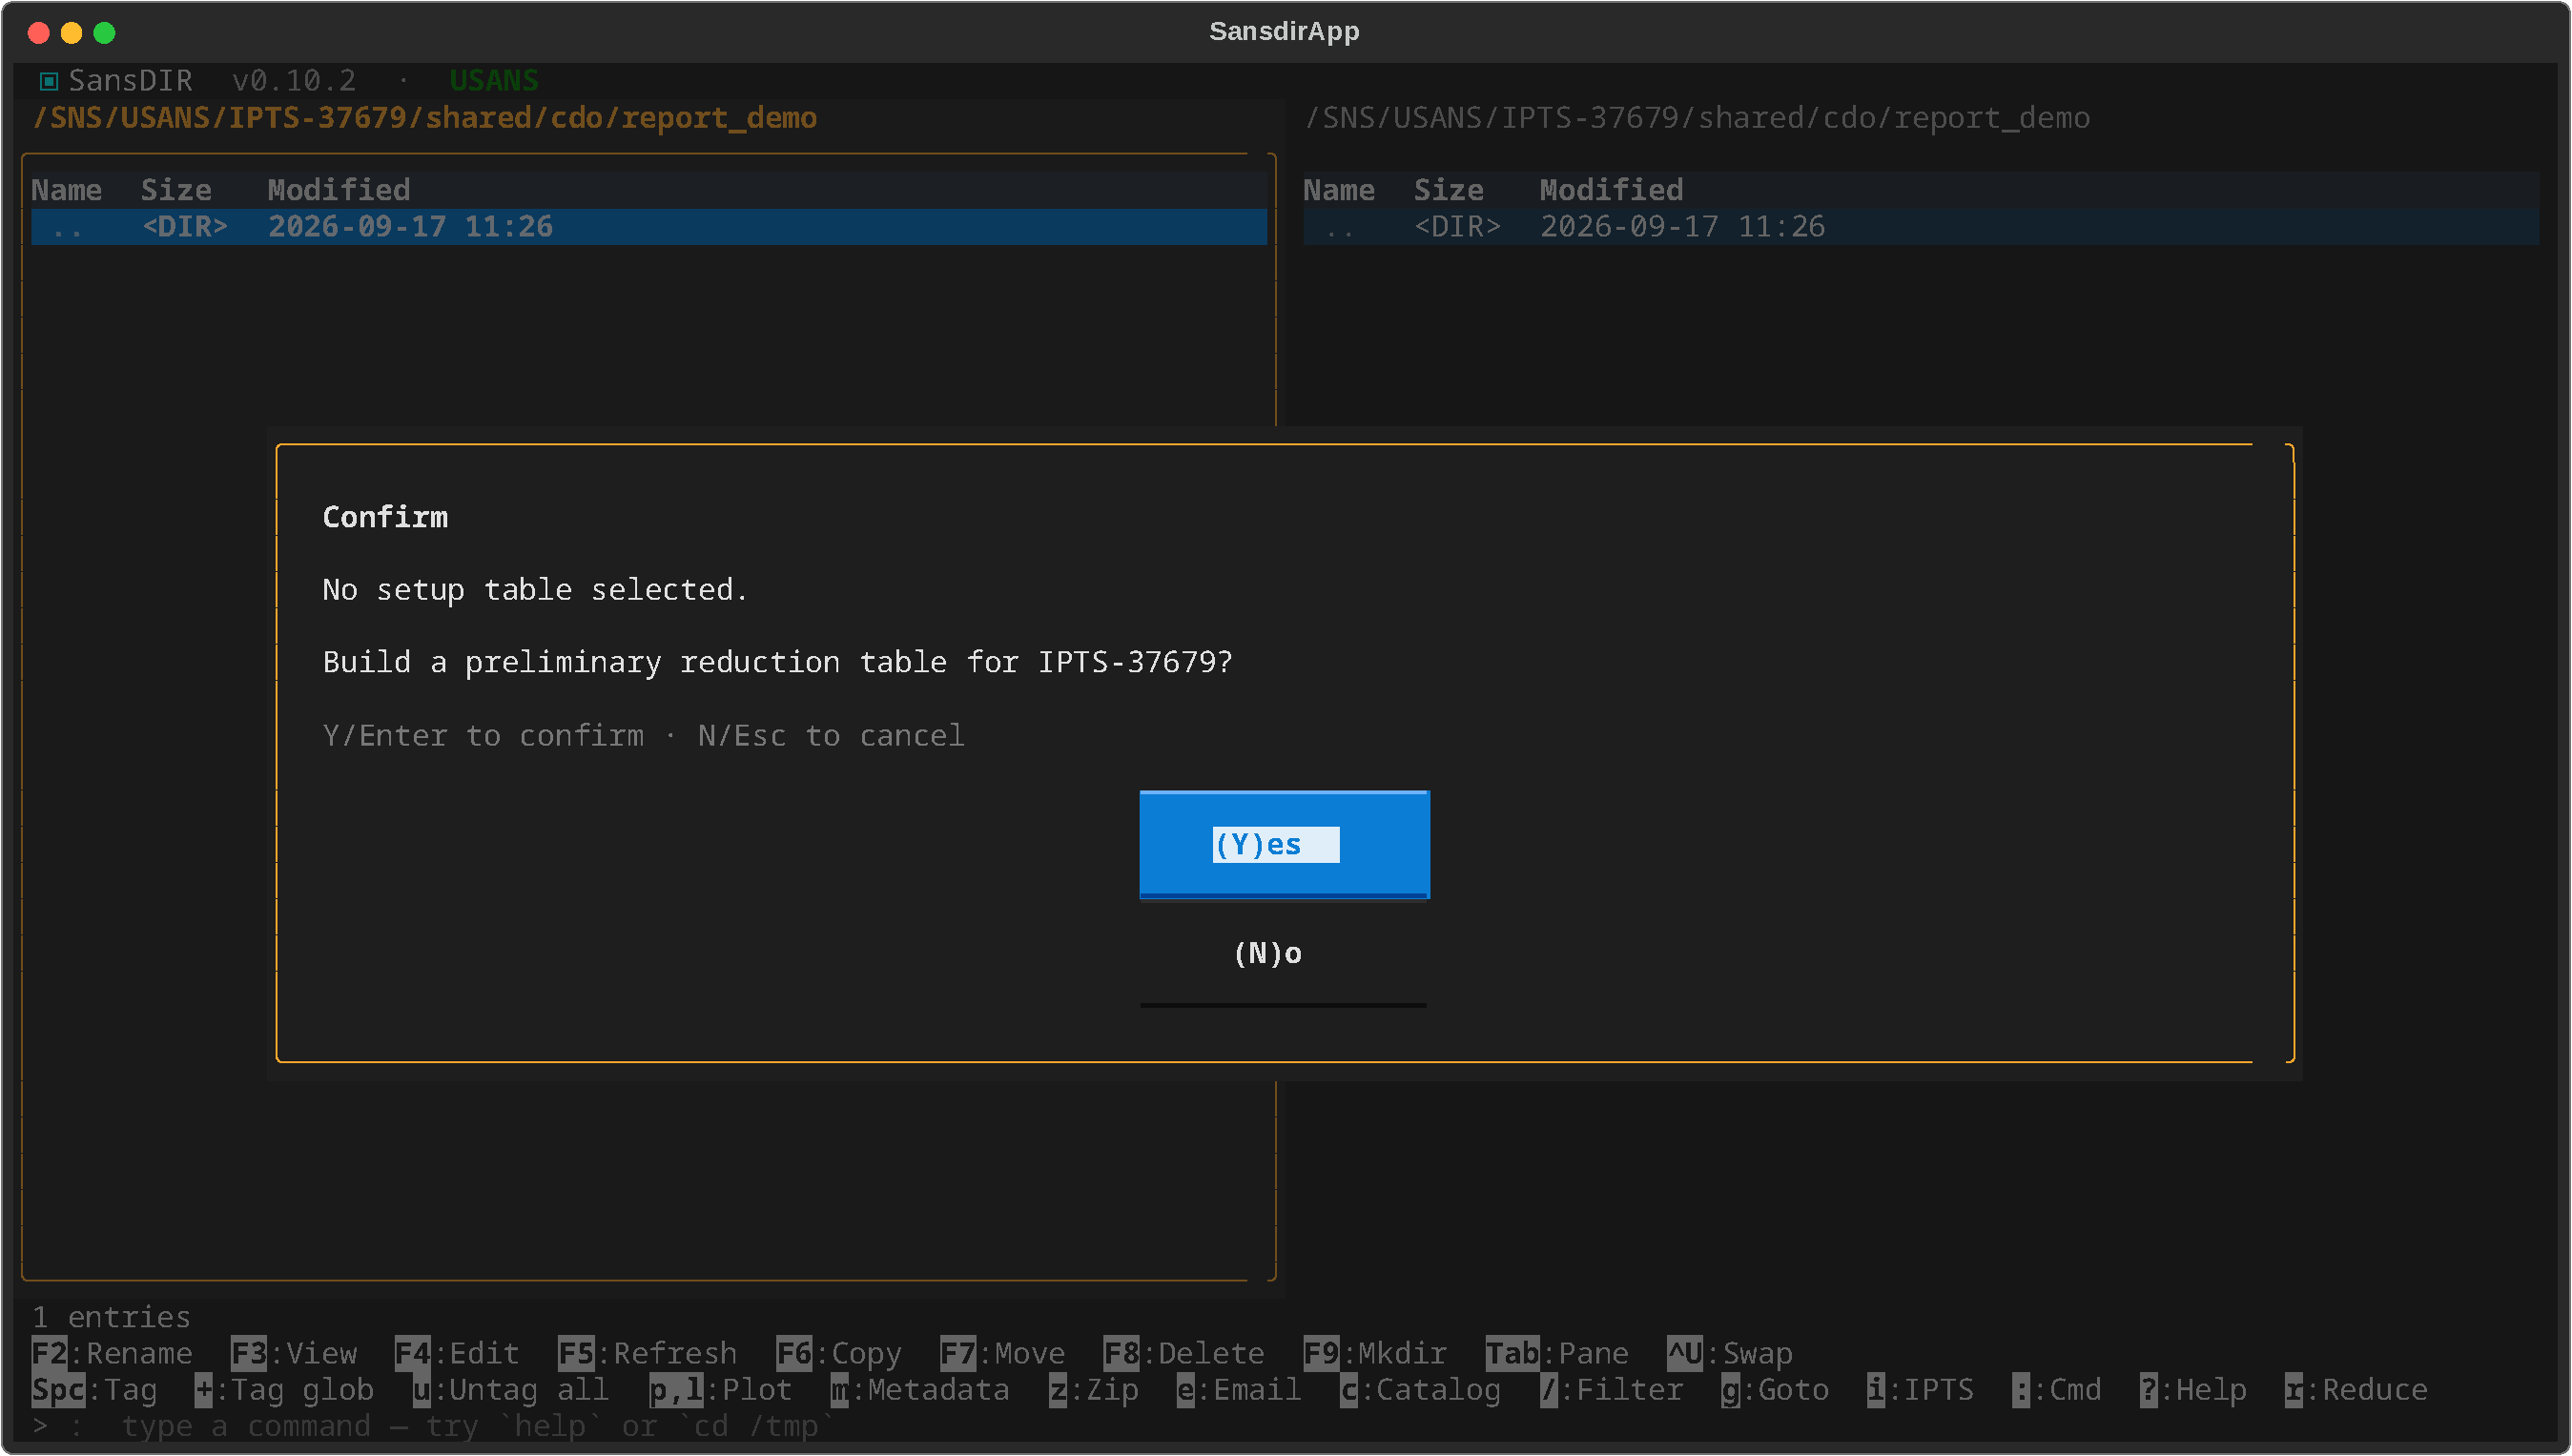
\includegraphics[width=\textwidth]{figures/usans-workflow-1.pdf}\\[1pt]
  {\small (a) \key{r} in an empty working folder: offer to build the setup table}\\[8pt]
  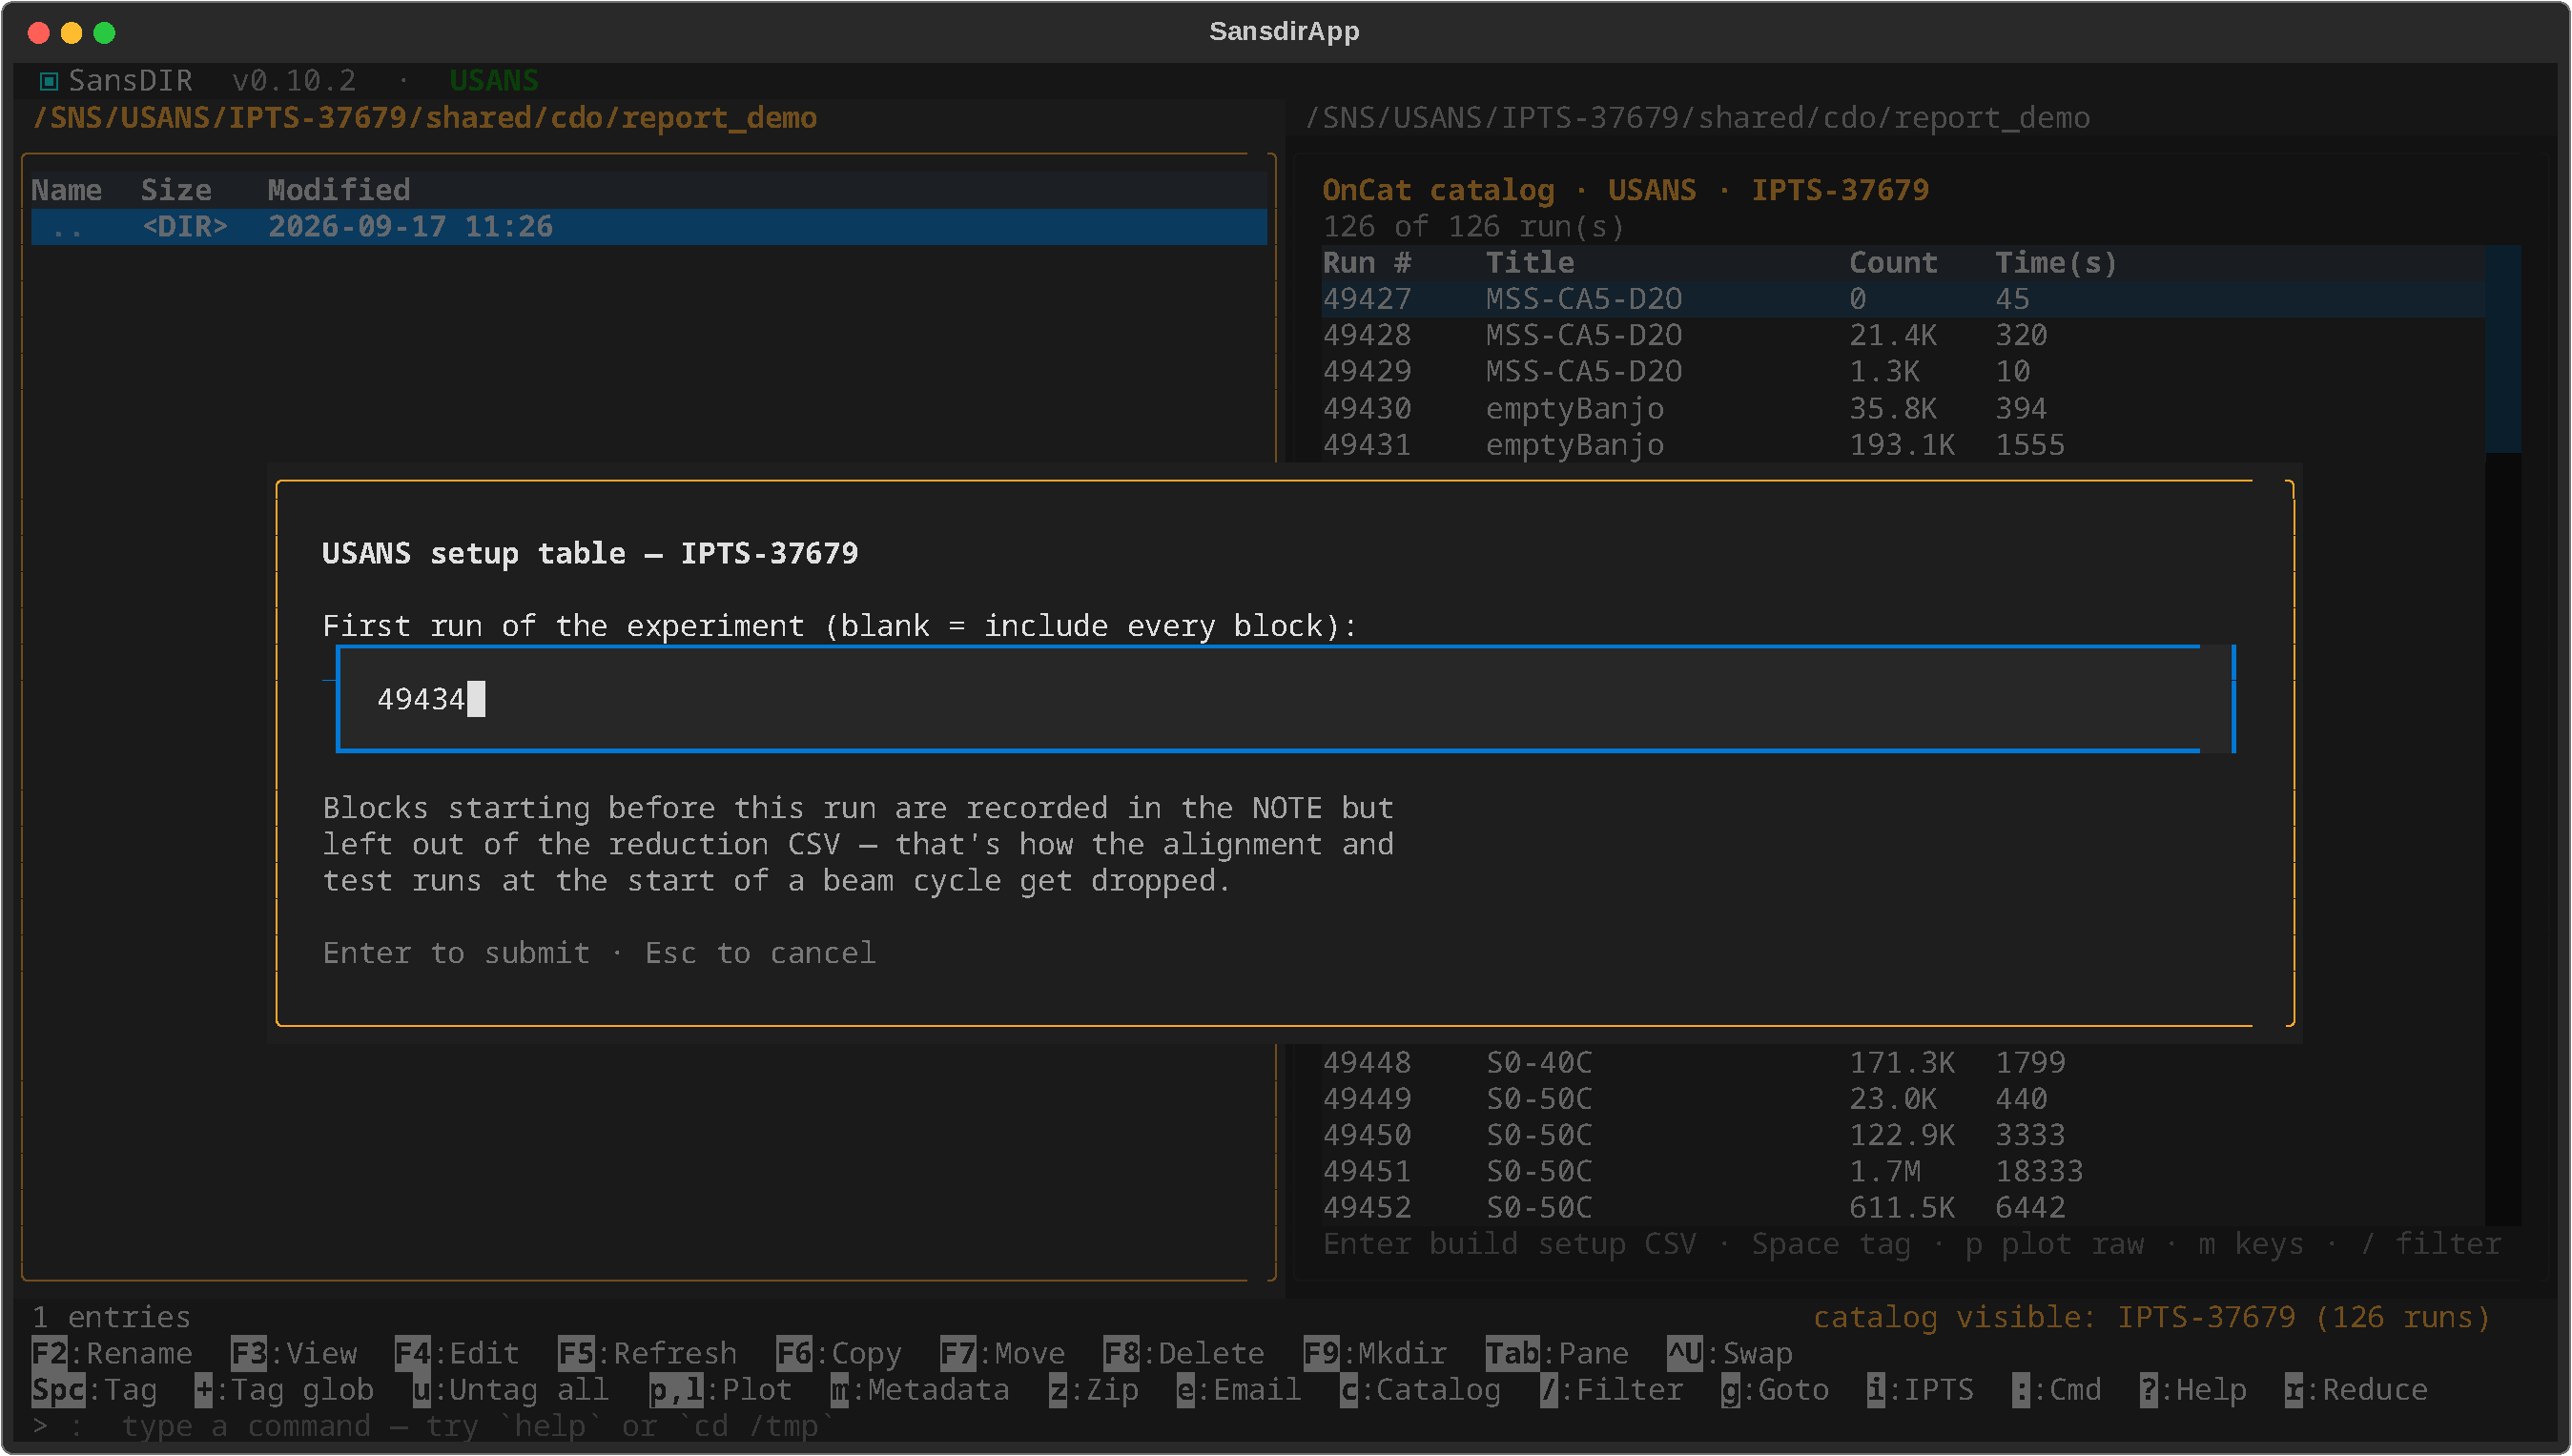
\includegraphics[width=\textwidth]{figures/usans-workflow-2.pdf}\\[1pt]
  {\small (b) the start-of-experiment prompt: run 49434}
  \longcaption{USANS reduction, end to end, on one key (1 of 2).}{(a)~\key{r}
  in an empty working folder offers to build the setup table for the IPTS
  named by the path. (b)~The start-of-experiment prompt (run 49434); the
  fetched run list is visible in the other pane.}
  \label{fig:usans-workflow}
\end{figure}

\begin{figure}[p]
  \centering
  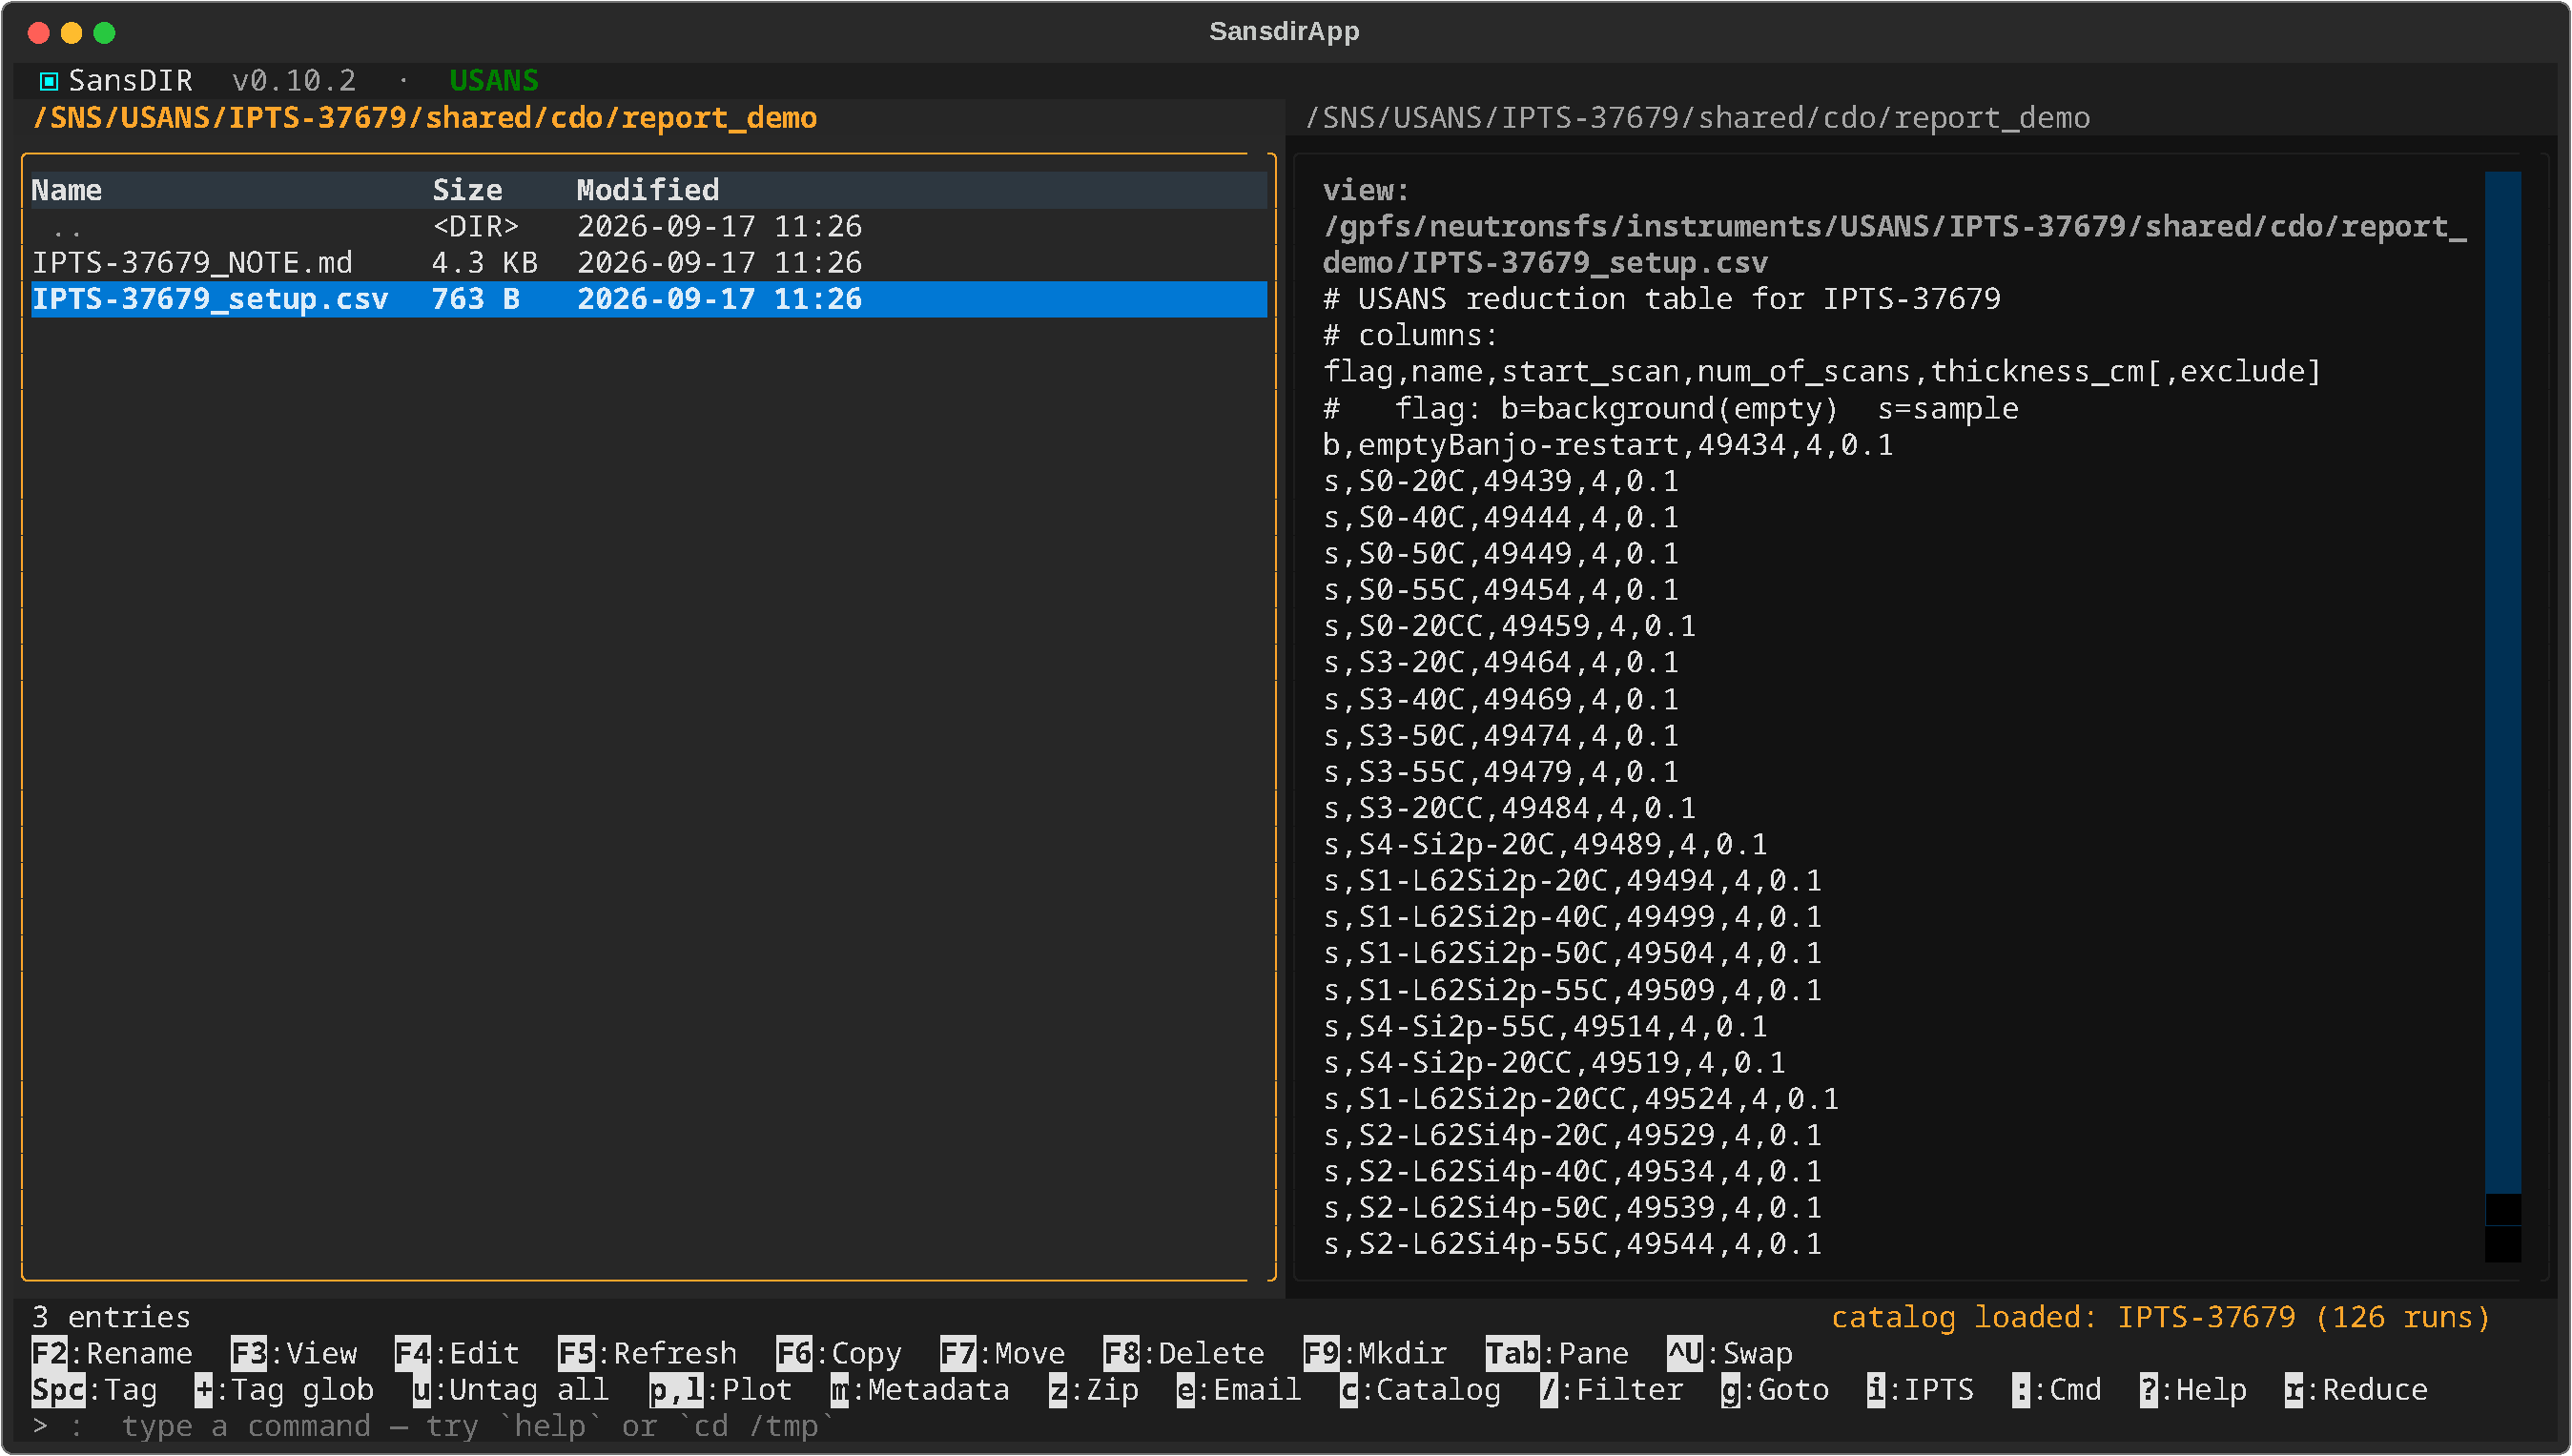
\includegraphics[width=\textwidth]{figures/usans-workflow-3.pdf}\\[1pt]
  {\small (c) the generated setup CSV, previewed in the other pane}\\[8pt]
  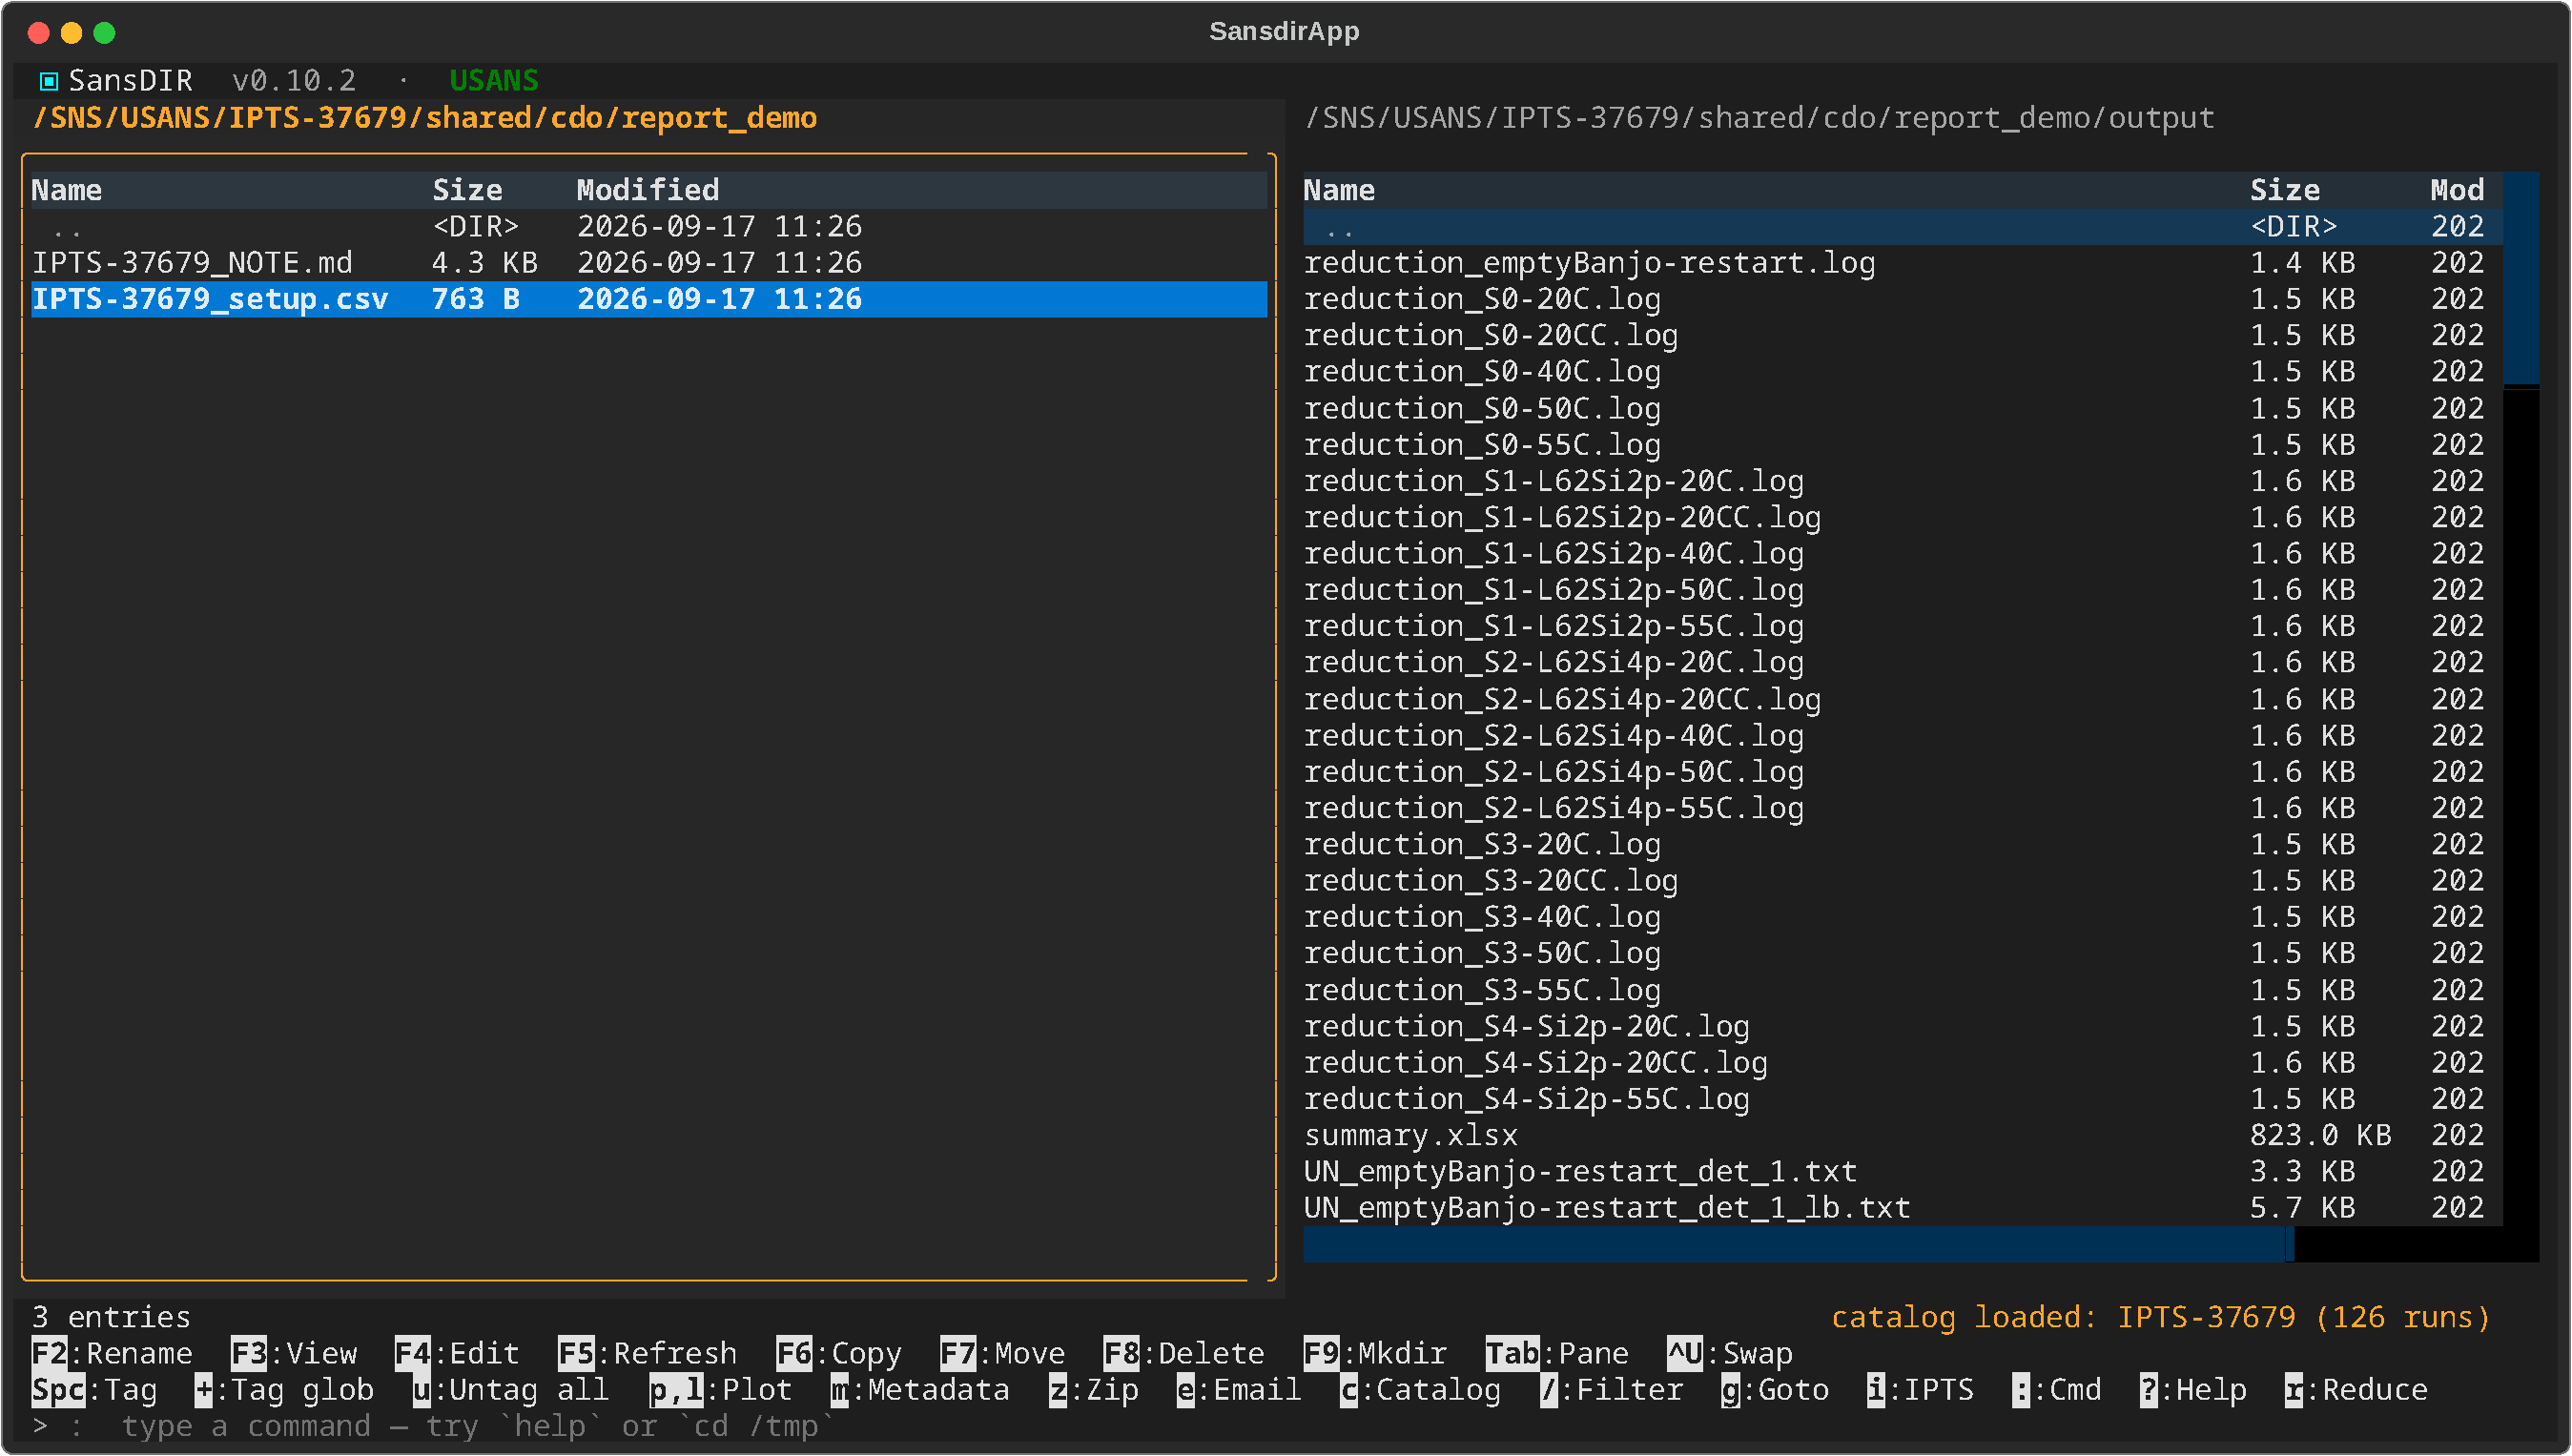
\includegraphics[width=\textwidth]{figures/usans-workflow-4.pdf}\\[1pt]
  {\small (d) after the second \key{r}: the reduced curves in the other pane}
  \longcaption{USANS reduction, end to end, on one key (2 of 2).}{(c)~The
  generated table under the cursor, previewed in the other pane for review.
  (d)~After the second \key{r}: the reduced curves in the output folder.}
  \label{fig:usans-workflow-2}
\end{figure}

\subsection{DESMEARING}
\label{sec:desmear}

\Ac{usans} instruments use slit collimation instead of pinhole collimation. The
larger illuminated area provides the flux needed for the high angular resolution
of the Bonse--Hart crystal optics. However, the intensity recorded at a nominal
momentum transfer $Q$ is an average of the true intensity over the vertical
acceptance,
%
\begin{equation}
  I_\text{exp}(Q) = \frac{1}{\sigma_y}\int_0^{\sigma_y}
    I\!\left(\sqrt{Q^2 + s^2}\,\right)\,\mathrm{d}s,
  \label{eq:smear}
\end{equation}
%
where $\sigma_y$ is the vertical resolution half-width. For the \ac{sns}
instrument, $\sigma_y \simeq 0.13~\text{\AA}^{-1}$, which is two decades above
the top of the measured window. Desmearing recovers $I(Q)$ from
$I_\text{exp}(Q)$. This is an ill-posed problem because the slit average couples
each measured point to scattering at much higher $Q$.

The \key{d} key desmears the selected reduced curves. The program uses the
non-iterative truncated Abel inversion of Huang \autocite{huang2026abel}. The
method expresses the intrinsic intensity in closed form as
%
\begin{equation}
  I(Q) = I(Q_m) - \frac{2\sigma_y}{\pi}
    \int_Q^{Q_m}\frac{I_\text{exp}'(Q_x)}{\sqrt{Q_x^2 - Q^2}}\,\mathrm{d}Q_x,
  \qquad Q_m = \sqrt{Q^2 + \sigma_y^2}.
  \label{eq:abel}
\end{equation}
%
Because the expression is closed-form, the program propagates uncertainty
through one linear operator instead of across iterative updates. This differs
from the widely used iterative Lake method \autocite{lake1967}. Each integral is
evaluated with the substitution $Q_x = \sqrt{Q^2 + s^2}$, which removes the
$1/\sqrt{Q_x^2 - Q^2}$ singularity at the lower limit. A Bayesian
Gaussian-process alternative has also been reported for this inversion
\autocite{tung2026gpr}.
The program uses the Abel method because it is deterministic and provides
closed-form error propagation.

Equation~\eqref{eq:abel} evaluates $I$ at $Q_m \simeq \sigma_y$ and integrates
to that point. Therefore, it requires scattering data well beyond the
\ac{usans} window. This requirement produces one interactive choice. When one
curve is selected, the program asks whether a companion pinhole \ac{sans}
measurement of the same sample is available. The question appears in the current
pane, while the other pane remains a filterable file list. If a companion curve
is selected, the two curves are placed on a common smearing basis, scale-matched,
joined across the instrument gap, and inverted over the full range. If the user
declines, or if several curves are desmeared together, the high-$Q$ side is
extrapolated as a power law to $\sigma_y$. This is the approach used by the
\ac{nist} \textsc{Igor}/\textsc{Irena} package \autocite{kline2006}. The result
is then limited to the measured \ac{usans} range, and the extrapolation is
recorded in the output header. Huang \autocite{huang2026abel} show that a
reconstruction without measured high-$Q$ data is reliable only at low $Q$. The
limited output range and header note make this restriction visible.

The desmeared curve is written as a three-column $Q$, $I$, $\mathrm{d}I$ text
file, which the \key{p} key plots in the same way as other curves. The inversion
uses only \texttt{numpy} and adds no dependency. It was validated by a
smear--desmear round trip using analytic power laws. The tests require the
recovered log--log slope to agree within 0.03 and the median core intensity error
to remain below two percent. The reported uncertainty increases near the top of
the range, where the high-$Q$ extrapolation is less reliable.

%%%%%%%%%%%%%%%%%%%%%%%%%%%%%%%%%%%%%%%%%%%%%%%%%%%%%%%%%%%%%%%%%%%%%%%%%%%%%%%
% 12. DATA FORMATS
%%%%%%%%%%%%%%%%%%%%%%%%%%%%%%%%%%%%%%%%%%%%%%%%%%%%%%%%%%%%%%%%%%%%%%%%%%%%%%%
\section{SUPPORTED DATA FORMATS}
\label{sec:formats}

\subsection{ASCII REDUCED DATA}

Reduced data files are whitespace-delimited ASCII. Optional comment lines begin
with \texttt{\#}. Table~\ref{tab:formats} lists the recognized column layouts.
The program counts the columns in the first non-comment line.

\begin{table}[ht]
  \centering
  \begin{threeparttable}
  \caption{Recognized ASCII column layouts}
  \label{tab:formats}
  \small
  \begin{tabular}{l c l p{0.34\textwidth}}
    \toprule
    Kind & Columns & Layout & Treatment \\
    \midrule
    \multirow{3}{*}{$I(q)$}
      & 2 & $q$, $I(q)$ & Logarithmic axes \\
      & 3 & $q$, $I(q)$, $\sigma_I$ & Logarithmic axes with error bars \\
      & 4 & $q$, $I(q)$, $\sigma_I$, $\sigma_q$ & As three-column; the
        resolution column is not plotted \\
    \midrule
    \multirow{2}{*}{Transmission}
      & 2 & $\lambda$, $T(\lambda)$ & Linear axes, $\lambda$ in \AA \\
      & 3 & $\lambda$, $T(\lambda)$, $\sigma_T$ & With error bars \\
    \midrule
    \multirow{2}{*}{$I(q_x,q_y)$}
      & 4 & $q_x$, $q_y$, $I$, $\sigma_I$ & Heat map on the recovered
        $q$ grid \\
      & 6 & $q_x$, $q_y$, $I$, $\sigma_I$, $dq_x$, $dq_y$ & As four-column \\
    \bottomrule
  \end{tabular}
  \begin{tablenotes}
    \item \emph{Note:} Classification does not rely on column count alone; the
    filename and any header keywords are considered first.
  \end{tablenotes}
  \end{threeparttable}
\end{table}

\subsection{NEXUS FILES}

Raw event-mode files follow the \ac{sns} NeXus conventions
\autocite{nexus}. The program uses the paths
\texttt{/entry/bank<N>\_events/event\_id} for detector events,
\texttt{/entry/instrument/bank1/pixel\_id} when an explicit pixel-identifier
array is available,
\texttt{/entry/DASlogs/<name>/value} for sample environment values, and
\texttt{/entry/DASlogs/<name>/time} for the corresponding time axis. Scalars such
as \texttt{/entry/duration} are read directly.

Processed Mantid files are also accepted for detector viewing and metadata
extraction. Mantid writes these files with a \texttt{.nxs} extension but without
the \texttt{.h5} suffix. Therefore, classification checks the \ac{hdf} magic
signature instead of using only the filename.

%%%%%%%%%%%%%%%%%%%%%%%%%%%%%%%%%%%%%%%%%%%%%%%%%%%%%%%%%%%%%%%%%%%%%%%%%%%%%%%
% 13. TESTING
%%%%%%%%%%%%%%%%%%%%%%%%%%%%%%%%%%%%%%%%%%%%%%%%%%%%%%%%%%%%%%%%%%%%%%%%%%%%%%%
\section{TESTING AND QUALITY ASSURANCE}
\label{sec:test}

\subsection{TEST SUITE}

For version 0.10.2, pytest collects 805 test cases from 51
\texttt{test\_*.py} modules. Six test functions are interface snapshot
comparisons. Integration tests that require a real NeXus file or the installed
reduction engine are skipped when those resources are not available. The exact
pass, skip, and run-time results depend on the test environment and are not used
as fixed values in this report.

The tests follow the software layers:

\begin{itemize}
  \item \textbf{Unit tests} cover every module under \texttt{core/},
    \texttt{hdf/}, \texttt{mask/}, and the plot classification logic.
  \item \textbf{Registry tests} verify duplicate-name rejection, parameter
    validation, argument checking during dispatch, and that every key binding
    names an existing command.
  \item \textbf{Interface tests} drive the real application through Textual's
    pilot harness, pressing keys and asserting on resulting state. The feature of
    Section~\ref{sec:hdfsearch}, for example, is covered by tests that press
    \key{/}, type a query, wait for the worker, and assert on the resulting
    match list, the case-insensitivity of the match, the two-stage \key{Esc}
    behavior, and the empty-result path.
  \item \textbf{Snapshot tests} compare rendered output against stored
    references to catch unintended layout regressions.
\end{itemize}

Two restrictions apply to the tests. OnCat tests use mock \ac{rest} responses
and do not contact the real service. Tests also do not access real cluster data
paths. Their fixtures are generated or taken from a small set of committed
files.

\subsection{STATIC ANALYSIS AND STYLE}

Linting and formatting use \texttt{ruff} with a line length of 100 and the
\texttt{E}, \texttt{F}, \texttt{W}, \texttt{I}, \texttt{B}, \texttt{UP},
\texttt{N}, \texttt{C4}, \texttt{SIM}, and \texttt{RUF} rule sets enabled.
Type checking uses \texttt{mypy} in strict mode over \texttt{src/sansdir}.
Public functions have type hints and Google-style docstrings. Bare
\texttt{except} clauses are not allowed. Exceptions are caught specifically,
logged, and shown to the user in the status bar.

\Ac{ci} runs the suite on Python 3.10, 3.11, and 3.12 on Linux.

%%%%%%%%%%%%%%%%%%%%%%%%%%%%%%%%%%%%%%%%%%%%%%%%%%%%%%%%%%%%%%%%%%%%%%%%%%%%%%%
% 14. PERFORMANCE
%%%%%%%%%%%%%%%%%%%%%%%%%%%%%%%%%%%%%%%%%%%%%%%%%%%%%%%%%%%%%%%%%%%%%%%%%%%%%%%
\section{PERFORMANCE}
\label{sec:perf}

Table~\ref{tab:perf} lists the performance budgets. Startup is measured. The
other values are targets used to identify regressions. When a target is missed,
the operation is profiled with \texttt{pyinstrument}.

\begin{table}[ht]
  \centering
  \begin{threeparttable}
  \caption{Performance measurement and regression budgets}
  \label{tab:perf}
  \small
  \begin{tabular}{p{0.55\textwidth} l l}
    \toprule
    Operation & Value & Basis \\
    \midrule
    \texttt{sansdir --help} startup & $\sim$120~ms median\tnote{a} & Measured \\
    Render a directory of 1,000 entries & 100~ms & Regression budget \\
    OnCat search, first call & 2~s & Regression budget \\
    OnCat search, cached & 100~ms & Regression budget \\
    Single metadata key read & 50~ms & Regression budget \\
    Batch extract, 100 files, 3 keys & 10~s & Regression budget \\
    \bottomrule
  \end{tabular}
  \begin{tablenotes}
    \item[a] Median end-to-end wall-clock time for \texttt{sansdir --help} on
    an analysis node, re-measured after the \ac{usans} reduction and desmearing
    features were added; the best case is near 60~ms. The figure did not grow
    with those features because the fast path imports none of the scientific
    stack (Section~\ref{sec:startup}).
  \end{tablenotes}
  \end{threeparttable}
\end{table}

Three measures help keep these operations within their budgets. Directory
listings use \texttt{os.scandir} and reuse each entry's stat result during one
scan. The OnCat browser debounces its filter input and limits the number of
rendered rows. \Ac{hdf} value previews take a slice before materializing an
array, so the preview cost does not depend on the full length of an event array.

%%%%%%%%%%%%%%%%%%%%%%%%%%%%%%%%%%%%%%%%%%%%%%%%%%%%%%%%%%%%%%%%%%%%%%%%%%%%%%%
% 15. LIMITATIONS AND FUTURE WORK
%%%%%%%%%%%%%%%%%%%%%%%%%%%%%%%%%%%%%%%%%%%%%%%%%%%%%%%%%%%%%%%%%%%%%%%%%%%%%%%
\section{SUMMARY}
\label{sec:future}

\textbf{sansdir} puts the file handling, inspection, and packaging tasks around
\ac{sans} reduction in one keyboard-driven terminal application. It also keeps
\ac{usans} setup, reduction, and desmearing in the same workflow. It does not
require a display server and runs from a shared installation on the \ac{ornl}
analysis cluster without per-user setup. The measured
\texttt{sansdir --help} startup has a median of about 120~ms; the \ac{tui}
first-paint time is not reported here.

Every interactive action is a typed command in one registry. Key bindings and
the interactive command line use this registry. The non-interactive Click
\ac{cli} uses a separate path to the same service functions. The command data
also generate the interactive help, while the service logic can be tested
without the terminal framework.

The present version has two main limitations. The detector heat map and mask
editor assume the EQ-SANS detector layout and have been tested only with
EQ-SANS data. The navigation and file-format operations are not specific to one
instrument, but they have not been verified on the \ac{hfir} \ac{sans}
instruments. Also, saving a mask that \texttt{drtsans} will use still requires a
Mantid environment, as described in Section~\ref{sec:mask}.

The \ac{usans} workflow in Section~\ref{sec:usans} has been tested from start to
end with data from one proposal. The grouping and scan-count checks use current
conventions: consecutive blocks with the same title, a transmission run at the
end, and an empty-cell title that names a banjo. These conventions apply to the
experiments examined but are not required by the data format. Therefore, the
program presents the generated table as a draft for review and does not reduce
it automatically.

Current work has two directions: creating \acp{doi} for tagged file sets through
the Zenodo \ac{api}, and adding a natural-language layer that translates a
free-text instruction into registry commands for user confirmation. Both would
use the existing command interface.

%%%%%%%%%%%%%%%%%%%%%%%%%%%%%%%%%%%%%%%%%%%%%%%%%%%%%%%%%%%%%%%%%%%%%%%%%%%%%%%
% ACKNOWLEDGMENTS
%%%%%%%%%%%%%%%%%%%%%%%%%%%%%%%%%%%%%%%%%%%%%%%%%%%%%%%%%%%%%%%%%%%%%%%%%%%%%%%
\section*{ACKNOWLEDGMENTS}

This research used resources at the \ac{sns}, a \ac{doe} Office of Science User
Facility operated by \ac{ornl}. Feedback from the first instrument scientist to
use the mask editor with production data led to substantial changes in its
interaction design.

%%%%%%%%%%%%%%%%%%%%%%%%%%%%%%%%%%%%%%%%%%%%%%%%%%%%%%%%%%%%%%%%%%%%%%%%%%%%%%%
% REFERENCES
%%%%%%%%%%%%%%%%%%%%%%%%%%%%%%%%%%%%%%%%%%%%%%%%%%%%%%%%%%%%%%%%%%%%%%%%%%%%%%%
\section{REFERENCES}
\printbibliography[heading=none]

%%%%%%%%%%%%%%%%%%%%%%%%%%%%%%%%%%%%%%%%%%%%%%%%%%%%%%%%%%%%%%%%%%%%%%%%%%%%%%%
% APPENDICES
%%%%%%%%%%%%%%%%%%%%%%%%%%%%%%%%%%%%%%%%%%%%%%%%%%%%%%%%%%%%%%%%%%%%%%%%%%%%%%%
\appendix
\acresetall

\section{COMMAND REGISTRY REFERENCE}
\label{sec:appcommands}

Table~\ref{tab:allcommands} lists all commands registered in version 0.10.2.
Each command can be entered on the \key{:} line by its name or alias.

\begin{small}
\begin{longtable}{p{0.24\textwidth} p{0.20\textwidth} p{0.46\textwidth}}
  \caption{Registered commands. A trailing question mark marks an optional
    parameter}
  \label{tab:allcommands} \\
  \toprule
  Command (alias) & Parameters & Description \\
  \midrule
  \endfirsthead
  \multicolumn{3}{l}{\emph{Table \ref{tab:allcommands}, continued. A trailing
    question mark marks an optional parameter.}} \\
  \toprule
  Command (alias) & Parameters & Description \\
  \midrule
  \endhead
  \bottomrule
  \endfoot
  \texttt{app.browse\_tree} & \texttt{root?} & Open a directory tree browser;
    the selected directory becomes the active pane's. \\
  \texttt{app.cmdline\_open} & --- & Focus the command line. \\
  \texttt{app.cmdline\_prompt} & \texttt{text} & Open the command line
    pre-filled. \\
  \texttt{app.help} (\texttt{help}) & --- & Show the help overlay. \\
  \texttt{app.quit} (\texttt{quit}, \texttt{q}) & --- & Exit. \\
  \texttt{archive.tar\_gz} (\texttt{tar}) & \texttt{srcs}, \texttt{out\_path} &
    Create a gzip-compressed tar archive. \\
  \texttt{archive.zip} & \texttt{srcs}, \texttt{out\_path} & Create a zip
    archive. \\
  \texttt{edit.file} (\texttt{edit}) & \texttt{path} & Edit in
    \texttt{\$EDITOR}. \\
  \texttt{file.copy} & \texttt{srcs}, \texttt{dst\_dir} & Copy into a
    destination directory. \\
  \texttt{file.delete} & \texttt{paths}, \texttt{trash?} & Delete or trash. \\
  \texttt{file.mkdir} (\texttt{mkdir}) & \texttt{name} & Create a directory. \\
  \texttt{file.move} & \texttt{srcs}, \texttt{dst\_dir} & Move, or rename a
    single file. \\
  \texttt{hdf.batch\_extract} (\texttt{extract}) & \texttt{paths},
    \texttt{keys}, \texttt{out?}, \texttt{fmt?}, \texttt{with\_stats?} &
    Extract log values from many NeXus files into a table. \\
  \texttt{hdf.show\_keys} (\texttt{hdf}) & \texttt{path} & Open the \ac{hdf}
    tree browser. \\
  \texttt{instrument.set} (\texttt{instrument}) & \texttt{name?} & Switch the
    session between \ac{sans} and \ac{usans}. \\
  \texttt{mail.send} & \texttt{recipient}, \texttt{subject?},
    \texttt{attachments?}, \texttt{body?} & Send mail via the configured
    client. \\
  \texttt{nav.cd} (\texttt{cd}) & \texttt{path} & Change the active pane's
    directory. \\
  \texttt{nav.up} & --- & Ascend one directory. \\
  \texttt{oncat.search} (\texttt{ipts}) & \texttt{keyword?},
    \texttt{instrument?} & Browse OnCat experiments. \\
  \texttt{pane.activate} & \texttt{panel\_id} & Activate the named pane. \\
  \texttt{pane.swap} & --- & Swap the two panes. \\
  \texttt{pane.sync} & --- & Match the inactive pane to the active one. \\
  \texttt{pane.toggle\_catalog} & --- & Flip the inactive pane between file list
    and run catalog. \\
  \texttt{pane.toggle\_max} & --- & Maximize or restore the active pane. \\
  \texttt{plot.detector\_sum} & \texttt{paths} & Render NeXus detector banks as
    heat maps. \\
  \texttt{plot.generic} (\texttt{plot.linear}, \texttt{lplot}) &
    \texttt{paths} & Linear plot of any tabular file. \\
  \texttt{plot.image} (\texttt{image}, \texttt{view.image}) & \texttt{paths} &
    Open image files in matplotlib. \\
  \texttt{plot.iq} & \texttt{paths} & Overlay 2-, 3-, or 4-column $I(q)$
    files. \\
  \texttt{plot.iqxqy} & \texttt{paths}, \texttt{colorbar\_mode?} & Plot 4-
    or 6-column $I(q_x,q_y)$ files; \texttt{colorbar\_mode} is \texttt{shared}
    or \texttt{independent}. \\
  \texttt{plot.transmission} & \texttt{paths} & Plot $T(\lambda)$ on linear
    axes. \\
  \texttt{shell.run} (\texttt{!}) & \texttt{cmd} & Run a shell command with the
    interface suspended. \\
  \texttt{tag.clear} & --- & Clear all tags in the active pane. \\
  \texttt{tag.glob} & \texttt{pattern} & Tag visible entries matching a
    glob. \\
  \texttt{tag.toggle} & \texttt{advance?} & Toggle the tag on the cursor
    row. \\
  \texttt{tag.untag\_glob} & \texttt{pattern} & Untag entries matching a
    glob. \\
  \texttt{ui.activate\_cursor} & --- & Context-sensitive \key{Enter}. \\
  \texttt{ui.batch\_extract} & \texttt{paths?} & Open the extraction dialog. \\
  \texttt{ui.copy\_tagged} & --- & Copy the selection to the inactive pane. \\
  \texttt{ui.delete\_tagged} & --- & Delete the selection, with
    confirmation. \\
  \texttt{ui.mail\_tagged} & --- & Mail the selection as attachments. \\
  \texttt{ui.mask} (\texttt{mask}) & \texttt{path?} & Open the mask editor. \\
  \texttt{ui.move\_tagged} & --- & Move the selection to the inactive pane. \\
  \texttt{ui.plot\_auto} & --- & Plot the selection, routing by file kind. \\
  \texttt{usans.init\_table} (\texttt{usans-init}) & \texttt{start\_run?},
    \texttt{out\_dir?}, \texttt{data\_dir?}, \texttt{ipts?} & Build a
    preliminary \ac{usans} setup \ac{csv} and notes. \\
  \texttt{usans.reduce} (\texttt{usans-reduce}) & \texttt{path?},
    \texttt{output\_dir?}, \texttt{data\_dir?}, \texttt{logbin?} & Reduce a
    setup \ac{csv}, or offer to build one. \\
  \texttt{usans.desmear} (\texttt{desmear}) & \texttt{paths?},
    \texttt{sans?}, \texttt{out\_dir?}, \texttt{sigma\_y?},
    \texttt{ask\_for\_sans?} & Desmear
    reduced \ac{usans} curves by truncated Abel inversion. \\
  \texttt{view.in\_other\_pane} & \texttt{path} & Show a file in the other pane
    (open, not toggle). \\
  \texttt{ui.plot\_generic} & --- & Linear plot of the selection. \\
  \texttt{ui.refresh} (\texttt{refresh}) & --- & Re-read both listings. \\
  \texttt{ui.rename} (\texttt{rename}) & --- & Rename the file under the
    cursor. \\
  \texttt{ui.set\_theme} (\texttt{theme}) & \texttt{name?} & Switch theme; no
    argument lists available names. \\
  \texttt{ui.zip\_tagged} & --- & Prompt for an archive path and zip the
    selection. \\
  \texttt{view.file} (\texttt{view}) & \texttt{path} & Open a read-only
    pager. \\
  \texttt{view.set\_filter} (\texttt{filter}) & \texttt{pattern?} & Filter the
    active pane; empty clears. \\
  \texttt{view.set\_sort} & \texttt{key}, \texttt{reverse?} & Set the sort
    key. \\
  \texttt{view.toggle\_hidden} & --- & Show or hide dotfiles. \\
  \texttt{view.toggle\_\allowbreak{}other\_pane} & --- & Show the cursor's file in the other
    pane. \\
\end{longtable}
\end{small}

\section{DEFAULT KEY MAP}
\label{sec:appkeys}

Table~\ref{tab:allkeys} lists the combined default map shown by the help overlay
in \ac{usans} mode. The \ac{sans} map omits \key{r} and \key{d}; the remaining
bindings are the same. Ten additional bindings are alternate terminal encodings
of the same keys and are not shown in the help overlay.

\begin{small}
\begin{longtable}{p{0.13\textwidth} p{0.40\textwidth} p{0.37\textwidth}}
  \caption{Default key bindings}
  \label{tab:allkeys} \\
  \toprule
  Key & Action & Command \\
  \midrule
  \endfirsthead
  \multicolumn{3}{l}{\emph{Table \ref{tab:allkeys}, continued}} \\
  \toprule
  Key & Action & Command \\
  \midrule
  \endhead
  \bottomrule
  \endfoot
  \key{Tab} & Switch the active pane & \texttt{pane.activate} \\
  \key{Ctrl+U} & Swap the two panes & \texttt{pane.swap} \\
  \key{=} & Sync the inactive pane & \texttt{pane.sync} \\
  \key{Ctrl+O} & Maximize or restore & \texttt{pane.toggle\_max} \\
  \key{Enter} & Open a directory, image, or text file &
    \texttt{ui.activate\_cursor} \\
  \key{Backspace} & Ascend one directory & \texttt{nav.up} \\
  \key{Space} & Tag or untag the current row & \texttt{tag.toggle} \\
  \key{+} & Tag by glob & \texttt{app.cmdline\_prompt} \\
  \key{-} & Untag by glob & \texttt{app.cmdline\_prompt} \\
  \key{u} & Untag all & \texttt{tag.clear} \\
  \key{h} & Toggle hidden files & \texttt{view.toggle\_hidden} \\
  \key{1} \key{2} \key{3} \key{4} & Sort by name, time, size, extension &
    \texttt{view.set\_sort} \\
  \key{F2} & Rename & \texttt{ui.rename} \\
  \key{F3} & View in the other pane & \texttt{view.toggle\_other\_pane} \\
  \key{F4} & Edit & \texttt{edit.file} \\
  \key{F5} & Refresh both panes & \texttt{ui.refresh} \\
  \key{F6} & Copy to the other pane & \texttt{ui.copy\_tagged} \\
  \key{F7} & Move to the other pane & \texttt{ui.move\_tagged} \\
  \key{F8} & Delete & \texttt{ui.delete\_tagged} \\
  \key{F9} & Make directory & \texttt{app.cmdline\_prompt} \\
  \key{g} & Jump to a path & \texttt{app.cmdline\_prompt} \\
  \key{G} & Browse the filesystem tree & \texttt{app.browse\_tree} \\
  \key{/} & Filter the active pane & \texttt{app.cmdline\_prompt} \\
  \key{c} & Toggle the run catalog & \texttt{pane.toggle\_catalog} \\
  \key{i} & OnCat proposal search & \texttt{oncat.search} \\
  \key{p} & Plot the selection & \texttt{ui.plot\_auto} \\
  \key{l} & Linear plot of the selection & \texttt{ui.plot\_generic} \\
  \key{m} & \Ac{hdf} metadata tree & \texttt{hdf.show\_keys} \\
  \key{M} & Batch metadata extract & \texttt{ui.batch\_extract} \\
  \key{K} & Create a detector mask & \texttt{ui.mask} \\
  \key{z} & Zip the selection & \texttt{ui.zip\_tagged} \\
  \key{e} & Email the selection & \texttt{ui.mail\_tagged} \\
  \key{:} & Open the command line & \texttt{app.cmdline\_open} \\
  \key{?} & Help overlay & \texttt{app.help} \\
  \key{r} & Reduce a \ac{usans} setup table (\ac{usans} mode only) &
    \texttt{usans.reduce} \\
  \key{d} & Desmear the selected \ac{usans} curves (\ac{usans} mode only) &
    \texttt{usans.desmear} \\
  \key{q} & Quit & \texttt{app.quit} \\
\end{longtable}
\end{small}

\section{WORKED EXAMPLE SESSION}
\label{sec:appsession}

The following sequence is an example of a data-triage session and uses most of
the program's features. It assumes that the proposal exists and that reduced
data are available.

\begin{enumerate}
  \item Launch with \texttt{sansdir}.
  \item Press \key{i} to open the OnCat browser. Press \key{/} to focus the
    filter, type a proposal number or a keyword from the title, and press
    \key{Enter} to move into the result list. Press \key{Enter} on the desired
    proposal and confirm. The active pane moves into the proposal's
    \texttt{shared/} directory and the run catalog loads on the right.
  \item Move into the catalog with \key{Tab}, scroll to a run of interest, and
    press \key{p} to view its raw detector image. Confirm the beam center and
    beam-stop placement, then close the plot window.
  \item Press \key{m} on the same run and then \key{/} to search for
    \texttt{temperature}. Confirm the sample environment value recorded for the
    run. Press \key{Esc} twice to return.
  \item Press \key{Tab} back to the file pane and descend into the reduction
    output directory.
  \item Tag the reduced curves to compare: press \key{+}, enter a glob such as
    \texttt{*20C*Iq.dat}, and press \key{Enter}. Press \key{p} to overlay them on
    logarithmic axes. Press \key{u} to clear the tags afterwards.
  \item Tag the corresponding transmission files and press \key{p} again; they
    are recognized as transmission data and drawn on linear axes.
  \item Press \key{M} to extract metadata across the run series. In the key
    picker, press \key{/}, search for the log of interest, press \key{Space} to
    select it, and press \key{Ctrl+S}. Choose summary mode and write the table.
  \item Press \key{l} on the resulting table to plot it directly.
  \item Tag the files to share, press \key{z}, and enter an archive name. Then
    tag the archive, press \key{e}, and complete the mail dialog.
  \item Press \key{q} to exit.
\end{enumerate}

%%%%%%%%%%%%%%%%%%%%%%%%%%%%%%%%%%%%%%%%%%%%%%%%%%%%%%%%%%%%%%%%%%%%%%%%%%%%%%%
\backmatter
\end{document}
%%%%%%%%%%%%%%%%%%%%%%%%%%%%%%%%%%%%%%%%%%%%%%%%%%%%%%%%%%%%%%%%%%%%%%%%%%%%%%%
